\newif\ifEN
\ENfalse   % \ENtrue = 英文投稿；\ENfalse = 中文工作版

\documentclass{SCIS2027}

\ifEN
  % 英文版不加载中文支持
\else
  \usepackage[UTF8, scheme=plain, autoindent=true]{ctex}
\fi

% SCIS2027.cls 已自带 amsmath/amsthm/amsfonts/amssymb/graphicx/algorithm/algorithmic/
% tabularx/url/float/booktabs/hyperref/cite/subfig 等，此处不再重复加载。
% 原 IEEEtran 模板中的 subcaption 已由 cls 内置的 subfig 替代（见 06_experiment.tex）。

% 图片目录
\graphicspath{{figures/}}

% 浮动体排版参数：避免多图连续堆进独立 float page，尽量与正文混排
\renewcommand{\floatpagefraction}{0.7}
\renewcommand{\textfraction}{0.15}
\setcounter{totalnumber}{3}
\renewcommand{\topfraction}{0.85}
\renewcommand{\bottomfraction}{0.7}

% 就地浮动体与正文的垂直间距
\setlength{\intextsep}{6pt plus 2pt minus 2pt}

% 浮动体之间、页顶/页底浮动体与正文的垂直间距
\setlength{\floatsep}{6pt plus 2pt minus 2pt}
\setlength{\textfloatsep}{12pt plus 2pt minus 2pt}

% 行间公式与正文的垂直间距（须在 \normalsize 之后生效，故置于 \AtBeginDocument）
\AtBeginDocument{
\setlength{\abovedisplayskip}{6pt plus 2pt minus 2pt}
\setlength{\belowdisplayskip}{6pt plus 2pt minus 2pt}
}

\begin{document}
%\oa

% ===== 期刊信息（投稿阶段留空）=====
\ArticleType{RESEARCH PAPER}
%\SpecialTopic{}
\Year{2027}
\Month{January}
\Vol{70}
\No{1}
\DOI{}
\ArtNo{}
\ReceiveDate{}
\ReviseDate{}
\AcceptDate{}
\OnlineDate{}
\AuthorMark{}
\AuthorCitation{}

% ===== 标题 =====
\title{Model-Based Reinforcement Learning for Continuous Forging Speed Control via a Latent World Model}{Model-Based Reinforcement Learning for Continuous Forging Speed Control via a Latent World Model}

% ===== 作者 =====
\author[1]{YiZhou Shao}{}
\author[2]{Zhaolin Yuan}{yuanzhaolin@ustb.edu.cn}
\author[3]{RuiZhe Wang}{}
\author[2]{XiaoKun Wang}{}

% ===== 单位 =====
\address[1]{School of Intelligence Science and Technology, University of Science and Technology Beijing, Beijing, China}
\address[2]{School of Intelligence Science and Technology, Shunde Innovation School, University of Science and Technology Beijing, Beijing, China}
\address[3]{School of Computer and Communication Engineering, University of Science and Technology Beijing, Beijing, China}

% ===== 摘要与关键词 =====
\ifEN
  \abstract{Forging is a core forming process in advanced equipment manufacturing, whose deformation is a strongly nonlinear, continuously evolving physical process. Capturing the complete evolution of geometry and multi-physics fields such as temperature, von Mises stress, and damage is key to improving forming quality and efficiency and to enabling rapid iteration of process parameters. However, while the traditional finite-element simulation is accurate, it requires numerically solving the entire deformation history, taking hours to days per run, and any change in process parameters necessitates full recomputation, making the cost difficult to amortize or reuse. Existing data-driven models, by contrast, mostly target single-point or low-dimensional time-series observations and rely on discrete-time modeling, so they can neither capture the high-dimensional, unordered, and massive forging point cloud and the spatiotemporal coupling of its multi-physics fields, nor incorporate the physical priors of the forging process. To address the above modeling challenges of high dimensionality, nonlinearity, and continuous evolution, this paper proposes a forging world model for forging deformation sequences, built on an Encoder--Latent Dynamics--Decoder architecture: a point-cloud encoder based on PointNet++ maps the high-dimensional point cloud into a low-dimensional latent state that jointly carries geometry and multi-physics information; a Neural ODE latent dynamics model incorporates the die speed profile as a physical prior into its time-scale transformation and models the continuous evolution of the latent state in an augmented ``physical-time--latent-state'' space, aligning the prediction time scale with the true process physics; and a joint geometry--physics decoder performs residual geometric reconstruction with the first-step geometry as the displacement base and regresses the physical fields by querying reference coordinates, thereby jointly predicting shape and multi-physics fields from a single latent state. The proposed method unifies the evolution of the ``geometry--multi-physics field'' of forging deformation into a continuously predictable latent-space dynamics, offering a new approach for the rapid prediction and process-parameter iteration of complex industrial processes such as forging.}
  \keywords{forging deformation sequence, forging world model, neural ordinary differential equation, multi-physics joint modeling}
\else
  \abstract{锻造是先进装备制造中的核心成形工艺，其变形是强非线性、连续演化的物理过程。获取锻造过程中几何形状与温度、等效应力、损伤等多物理场的完整演化，是提升成形质量与效率、支撑工艺参数快速迭代的关键；然而，传统有限元仿真虽精度高，却需数值求解完整变形历程，单次耗时数小时至数天，且工艺参数一变即需整体重算，难以摊销与复用；现有数据驱动模型则多面向单点或低维时序观测、以离散时间建模为主，既难以刻画高维、无序、体量庞大的锻造点云及其多物理场的时空耦合演化，也难以融入锻造工艺的物理先验。针对上述高维、非线性与连续演化的建模难题，本文提出一种面向锻造变形序列的锻造世界模型，采用“编码器—隐动力学—解码器”框架：点云编码器基于 PointNet++ 将高维点云映射为低维隐状态，统一承载几何与多物理场信息；神经常微分方程（Neural ODE）隐动力学模型将锻压速度曲线作为物理先验融入其时间尺度变换，在“物理时间—隐状态”增广空间中建模隐状态的连续演化，使预测的时间尺度与真实工艺物理一致；几何—物理场联合解码器以首步几何为位移基底进行残差式几何重建，并以参考坐标为查询回归物理场，从而在同一隐状态下联合预测形状与多物理场。所提方法将锻造变形的“几何—多物理场”演化统一建模为可连续预测的隐空间动力学，为锻造等复杂工业过程的快速预测与工艺参数迭代提供了一种新思路。}

  \keywords{锻造变形序列, 锻造世界模型, 神经常微分方程, 多物理场联合建模}
\fi

\maketitle

\ifEN
  \section{Introduction}

% ===== 第1段：业务问题（决策导向） =====
Forging is the primary forming process for load-bearing components in the aerospace, energy, and automotive sectors, where forming quality governs in-service safety and production efficiency and cost determine enterprise profitability. Forging production must therefore minimize forming time and maximize throughput while guaranteeing quality. As shown in Fig.~\ref{fig:forging_press}, the workpiece undergoes plastic deformation under compression between the upper and lower dies, and the die speed is the downward velocity of the upper die. This speed profile affects the thermo-mechanical response and dynamic softening of the material through its control of the strain rate~\cite{lin2011critical}, and simultaneously determines forging time and workpiece damage, thereby influencing throughput and quality~\cite{bambach2018towards}. How to set the die speed profile is thus the core decision problem for efficient, high-quality forging.

\begin{figure}[htbp]
\centerline{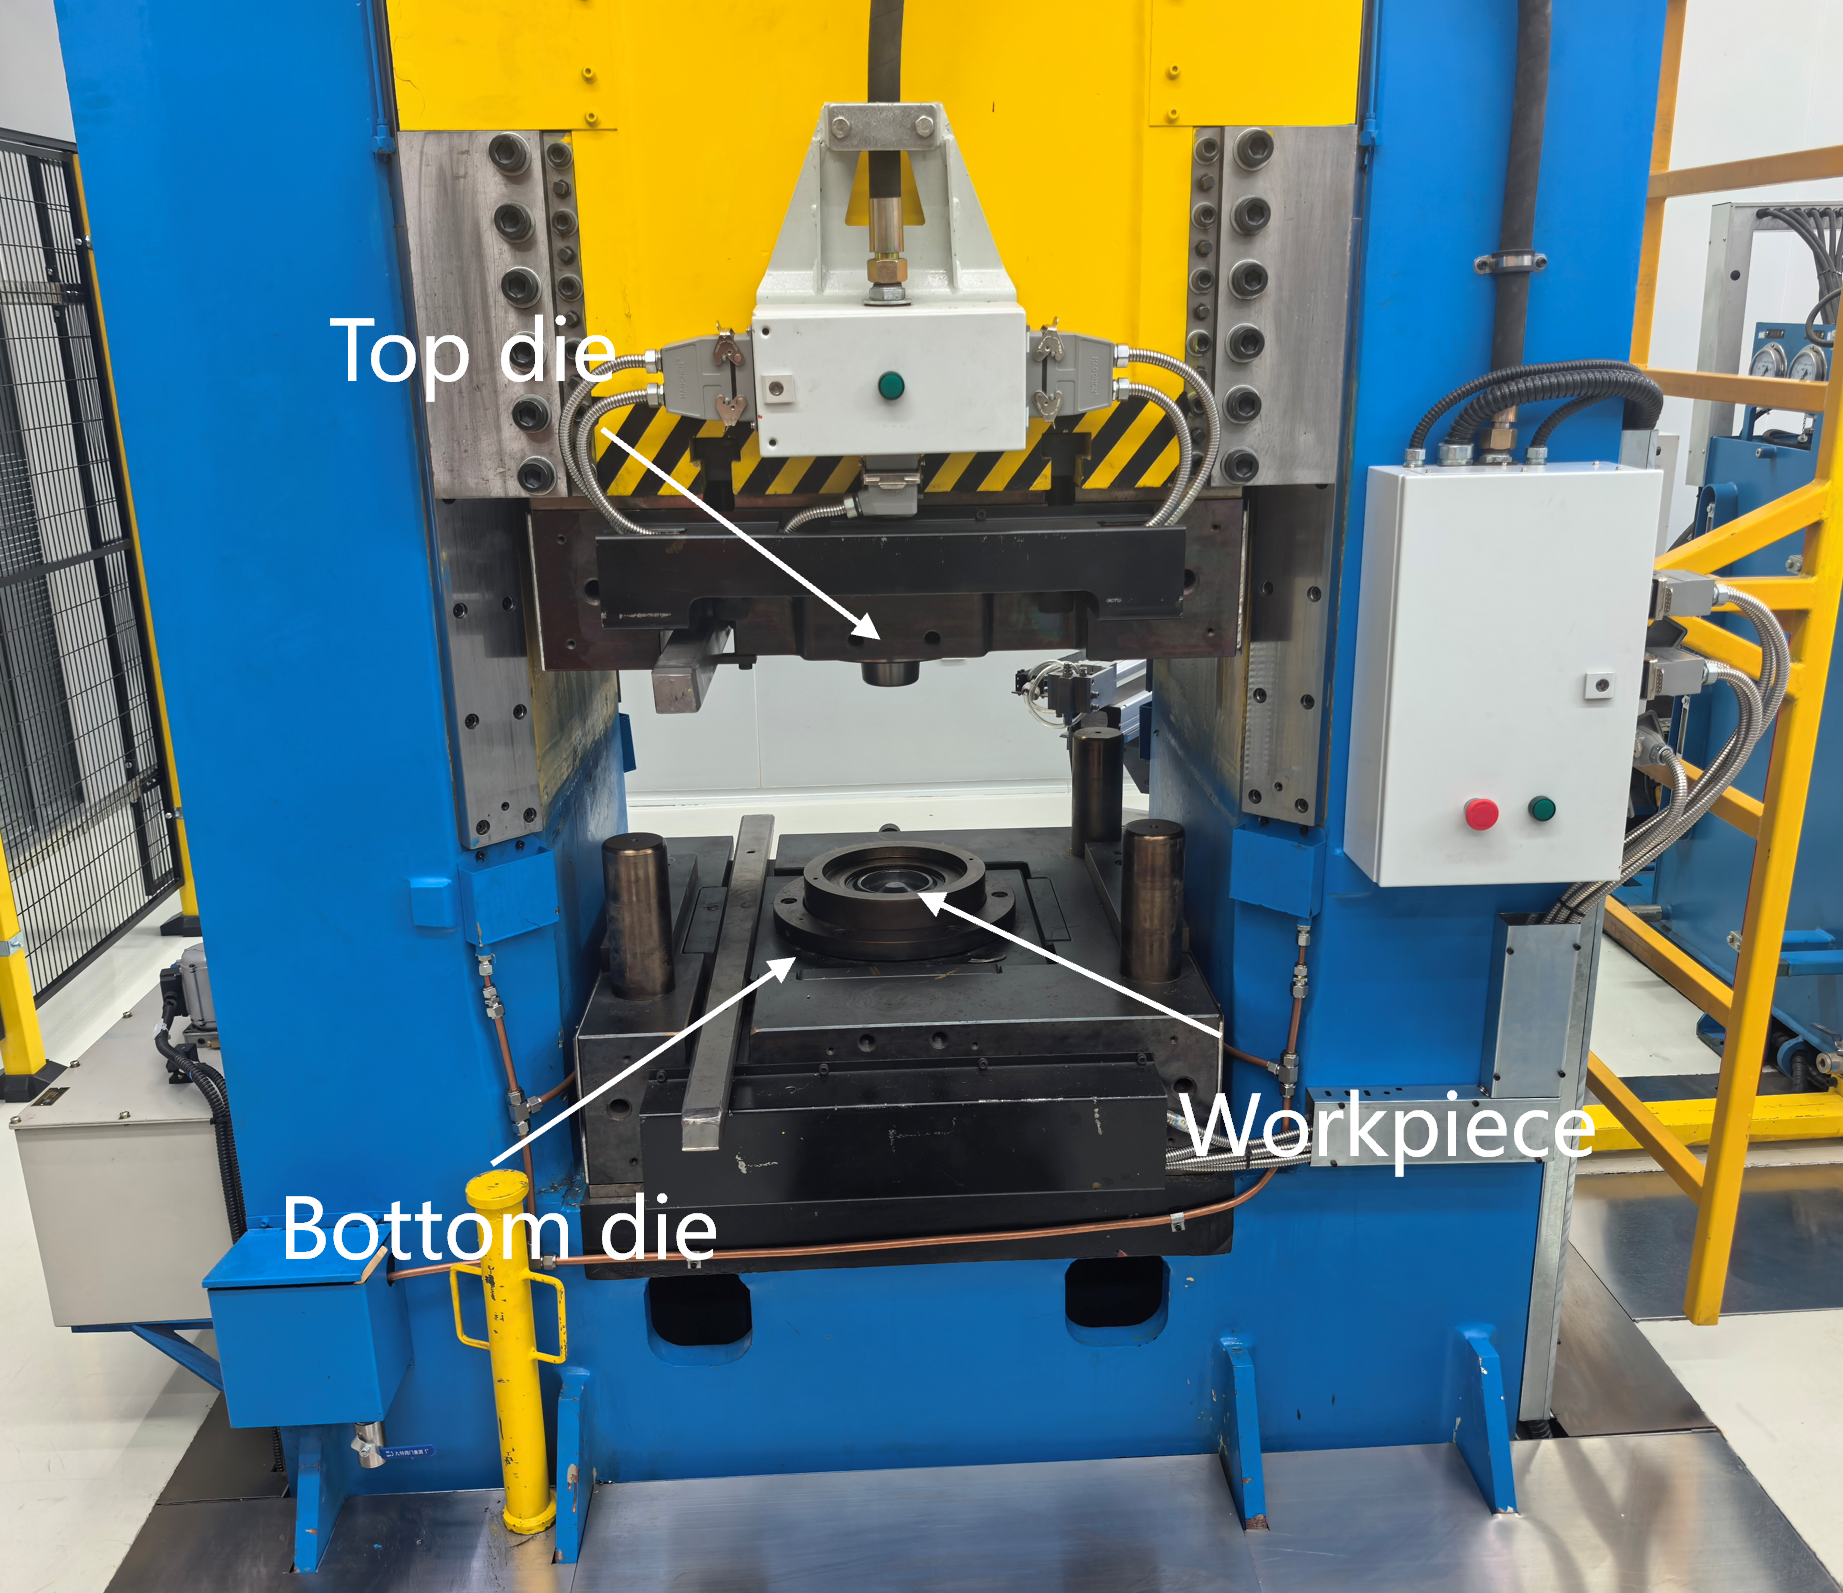
\includegraphics[width=7cm]{forging_press.png}}
\caption{Schematic of the forging press.}
\label{fig:forging_press}
\end{figure}

% ===== 第2段：研究意义（决策导向） =====
This work aims to intelligently determine the die speed profile under varying initial workpiece temperatures. Before forging, workpieces are preheated to different temperatures in a furnace; owing to transfer delays and differential heat loss between extraction and clamping, the initial temperature of each batch fluctuates, which in turn affects the deformation resistance and damage evolution throughout the process. Since the die speed can vary continuously over the entire forging history, the speed profile can flexibly modulate the pressing rate along with the evolution of temperature and deformation, minimizing forging time while keeping the workpiece free of cracking, and thereby raising throughput, lowering cost, and reducing equipment and die wear. Compared with constant-speed or low-dimensional piecewise schemes, a continuous speed profile offers higher degrees of freedom and process adaptability, exploiting the dynamic softening of the material more fully.

% ===== 第3段：已有工作①锻造工艺智能决策 =====
Existing work on intelligent decision-making for forging process parameters falls into three categories. Metaheuristic algorithms such as particle swarm optimization and NSGA-II search the parameter space with a finite-element or material model as the objective~\cite{chen2019strategy, ding2024enhancing}; however, each fitness evaluation requires a full simulation, and the optimized variables are mostly scalar parameters that cannot represent a speed profile varying continuously along the deformation history. Surrogate models instead fit a machine-learning mapping from process parameters to outcomes, such as predicting the strain distribution along the axis of a single pass~\cite{dischino2021open} or replacing finite elements with a graph neural network to predict the final-state field~\cite{shivaditya2022graph}; yet their outputs correspond to a single forming operation or one final state, lacking evolution along time steps and thus unable to provide the process state needed for stepwise decision-making. Control-based methods directly learn process policies, e.g., designing passes with deep Q-learning~\cite{reinisch2021successful}, and online adjustment of rolling speed~\cite{zhang2020online}, heating~\cite{ma2022using}, and TNM-B1 forging control~\cite{stendal2024developing}; but their actions are mostly discrete or low-dimensional setpoints and rely on online feedback, so they cannot provide a stepwise-adjustable continuous speed profile under offline conditions.

% ===== 第4段：已有工作②决策与控制方法 =====
A single forging operation is short, the internal stress and damage fields of the workpiece cannot be measured in real time, the temperature field can only be captured at the surface, and the system response latency is large; online closed-loop control based on real-time sensor feedback is thus impractical, and the speed profile can only be determined offline before production. Model predictive control requires online receding-horizon optimization and relies on real-time state feedback~\cite{kouvaritakis2016model}, but the internal state is unobservable and the latency is large, making receding-horizon optimization hard to implement. Iterative learning control depends on the repeatability of operating conditions~\cite{ahn2007iterative}, yet the temperature and clamping conditions of forging fluctuate batch by batch, so the repeatability assumption rarely holds. Online reinforcement learning requires repeated interaction with the environment~\cite{dharmadhikari2023reinforcement}, but forging experiments are costly and risky, making online exploration impractical. Offline reinforcement learning instead learns a policy from historical data~\cite{levine2020offline} and has been validated in process-industry scenarios such as hot rolling and thickeners~\cite{zhan2022deepthermal, 10705802}; however, its observations are mostly low-dimensional sensor readings and its actions are scalar setpoints, so it cannot accommodate point-cloud observations and function-level actions. World-model methods first learn environment dynamics in a latent space and then train or plan a policy within the model~\cite{hafner2020mastering}, but their constraints are typically formulated as cumulative costs and their execution is online closed-loop feedback, which is inconsistent with the requirements of the stepwise damage constraints and the one-shot offline deployment of this work.

% ===== 第5段：已有工作③点云表征 =====
The observation required for forging decision-making is a point cloud that carries geometry together with temperature, von Mises stress, and damage at every step. Point-cloud deep models, exemplified by PointNet++, extract permutation-invariant features through hierarchical sampling and local aggregation~\cite{qi2017pointnetpp}; however, these models target classification and segmentation of static scenes and output class or segmentation labels rather than physical fields. Point-cloud generation models such as PCN, FoldingNet, and PointFlow reconstruct or generate point clouds from a latent variable~\cite{yuan2018pcn, yang2018foldingnet, li2019pointflow}; yet their reconstruction target is a static point cloud, so they neither capture the time-varying evolution of the point cloud driven by process conditions nor predict the geometry and fields at the next moment from a latent state.

% ===== 第6段：已有工作④连续时间演化建模 =====
Forging thermo-mechanical deformation evolves continuously in time. The finite element method is highly accurate but requires numerically solving the entire deformation history, taking hours to days per run~\cite{halici2014modelling}; any change in process parameters necessitates a full recomputation, so the cost cannot be amortized. End-to-end data-driven models provide only a single input-to-output mapping and therefore lack multi-step temporal prediction capability. Sequential models such as RNNs, LSTMs, and Transformers recur over discrete time steps~\cite{elman1990finding, hochreiter1997long, vaswani2017attention}; however, discrete step sizes do not correspond to the continuous loading of forging, making it difficult to capture the continuous physical evolution. Neural ODEs describe the continuous change of state via a vector field, offering a framework for continuous-time modeling, yet their application to high-dimensional point-cloud multi-physics prediction remains limited. The temperature, stress, and damage of forging are fields defined over a continuous geometry that evolve along the deformation history and must be queried at arbitrary locations; existing data-driven models mostly discretize fields onto a fixed grid or a fixed number of points, making it difficult to predict the entire field on continuous coordinates. Operator-learning models such as DeepONet model a field as a continuous function of coordinates and learn function-to-function mappings: the branch encodes the function input, the trunk queries with the coordinate as the independent variable, and all points share a spatial basis, so that a single network outputs field values at arbitrary coordinates---matching the need to reconstruct a continuous geometry--multi-physics field from a low-dimensional latent state.

% ===== 第7段：本文思路 =====
To address the above limitations, this work constructs a forging world model that takes an arbitrary continuous-time speed profile as input and jointly carries the evolution of geometry and multi-physics fields in a low-dimensional latent state, characterizing the forging thermo-mechanical process in continuous time while guaranteeing reconstruction and multi-step prediction accuracy, serving as a surrogate environment for decision training and inference. Building on this model, a continuous speed-profile policy is trained from offline data to output a smooth, continuous, and directly executable speed profile that satisfies the damage constraint, thereby realizing intelligent decision-making of the die speed profile.

% ===== 第8段：研究方法 =====
This work adopts a two-stage method, with the overall framework shown in Fig.~\ref{fig:framework}.

\textbf{Stage 1: world model training.}
We adopt an Encoder--Latent Dynamics--Decoder architecture: a hierarchical PointNet++ encoder compresses the point cloud of each step into a low-dimensional latent state that jointly carries geometry and multi-physics information; a Neural ODE with the speed profile as a physical prior models the continuous-time dynamics in the latent space; and a decoder performs residual reconstruction with the first-step geometry as the displacement base and regresses the physical fields from the first-step coordinates, realizing reconstruction and prediction of the point cloud.

\textbf{Stage 2: policy training.}
With the trained world model as the environment, the speed-profile decision is formulated as a finite-horizon constrained Markov decision process with safety constraints; the policy takes the world model's latent state as input and determines the die speed step by step along the deformation history, generating a smooth, continuous speed profile; the policy is trained via offline safe reinforcement learning, with the damage constraint handled by Lagrangian relaxation. At solving time, the world model performs stepwise decision-making: at each step the current speed is output conditioned on the world model's latent state, so that the entire profile adapts to the process state without relying on physical sensors; after solving, the resulting complete speed profile is deployed to the equipment once.

\begin{figure}[htbp]
\centerline{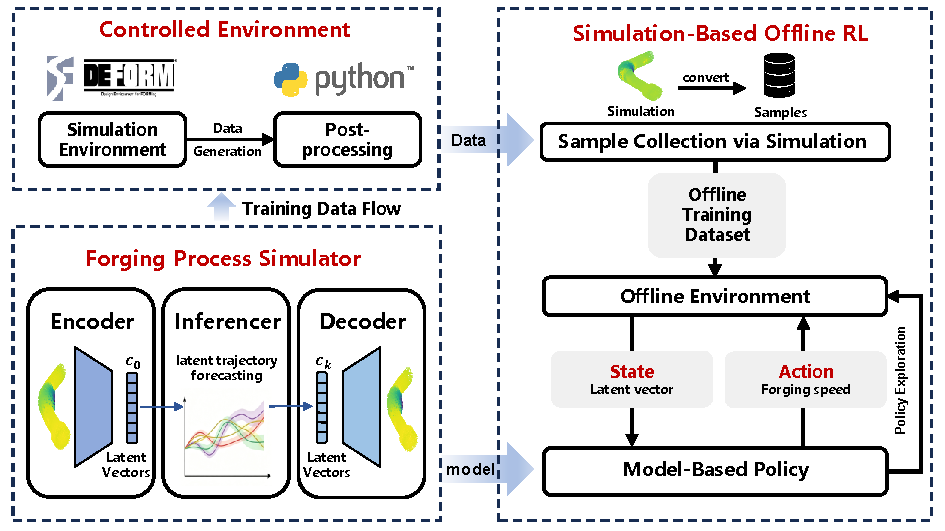
\includegraphics[width=12cm]{fram-1-wide.pdf}}
\caption{Overall framework of this work.}
\label{fig:framework}
\end{figure}

% ===== 第9段：研究贡献 =====
The main contributions are as follows:
\begin{enumerate}\setlength{\itemsep}{0pt}\setlength{\parsep}{0pt}
    \item \textbf{A forging world model for forging point-cloud sequences.}
    It jointly carries geometry and multi-physics fields in a low-dimensional latent state and models the controlled evolution process in continuous time via a Neural ODE, realizing reconstruction and multi-step prediction of the time-varying point-cloud process, and providing an efficient surrogate environment for decision training and inference.
    \item \textbf{Safe decision-making of continuous speed profiles based on the world model.}
    It solves offline within the world model to generate a smooth, continuous speed profile satisfying the damage constraint, which is then deployed to the equipment once, overcoming the representational limitations of conventional low-dimensional parameterization.
    \item \textbf{Practical validation.}
    The proposed method is applied to the forging of a 6082 aluminum alloy control arm, validating the prediction accuracy of the world model and the effectiveness of the decision scheme in the DEFORM simulation environment.
\end{enumerate}

  \section{Preliminaries}

\subsection{Point Cloud Representation}
A point cloud represents the workpiece surface as a set of three-dimensional points, where each point carries its coordinates together with physical quantities such as temperature and stress, denoted $X=\{x_i\}_{i=1}^{N}$ with $x_i\in\mathbb{R}^{C}$. A point cloud is an unordered set---the same shape corresponds to $N!$ orderings---so models operating on point clouds must be permutation-invariant~\cite{qi2017pointnet}. Unlike regular grids, a point cloud is free of topological and resolution constraints and can represent arbitrary geometries directly, making it suitable for carrying the geometry and fields output by finite-element simulations.

\subsection{Continuous-Time Latent State Modeling}
A Neural ODE describes the continuous evolution of a state via a parameterized vector field: given the initial value $c(s_0)=c_0$, the state at any position is obtained by integrating
\begin{equation}
\frac{\mathrm{d}c}{\mathrm{d}s}=g(c,s;\theta)
\end{equation}
~\cite{chen2018neural}. Compared with discrete-time recurrence, it characterizes the dynamics with a continuous independent variable, can be evaluated at arbitrary times, and supports backpropagation via the adjoint method. Such models have been applied to continuous-time modeling of industrial processes~\cite{yuan2022autonomous, yuan2023ode, yuan2022differential}.

\subsection{World Model}
A world model compresses high-dimensional observations into a low-dimensional latent state and learns the evolution of the state under actions in the latent space, thereby predicting the future without interacting with the real environment. A typical structure consists of an encoder, a latent dynamics model, and a decoder: the encoder maps observations to the latent state, the latent dynamics model predicts the latent state at the next time, and the decoder reconstructs observations from the latent state. Prediction is performed in the low-dimensional space, whose cost is far lower than reasoning directly over high-dimensional observations.

\subsection{DeepONet}
DeepONet learns function-to-function mappings and consists of two sub-networks, branch and trunk: the branch receives discrete samples of the input function, the trunk receives the independent variable of the output function, and the inner product of their outputs yields the function value at that variable~\cite{lu2021deeponet}. Since the output is a continuous function of the independent variable, the model can produce predictions at arbitrary locations without pre-fixing a discrete grid.

  \section{Problem Formulation}

\subsection{Forging Deformation Sequence and State Representation}
During aluminum alloy forging, the workpiece undergoes plastic deformation under compression between the upper and lower dies, and its geometry together with physical quantities such as temperature, von Mises stress, and damage evolve synchronously and continuously along the deformation history. The workpiece state at step $k$ of the forging process is represented by an unordered point cloud $X_k \in \mathbb{R}^{N \times 6}$, where $N$ is the number of sampled points and each point consists of the absolute coordinate $p_i=(x_i,y_i,z_i)$ and three physical fields---temperature $T_i$, von Mises stress $\sigma_i$, and damage $D_i$:
\begin{equation}
X_k = \{\,(p_i,\; T_i,\; \sigma_i,\; D_i)\,\}_{i=1}^{N}
\label{equ:pointcloud}
\end{equation}
where the von Mises stress is composed from the six stress components by physical magnitude:
\begin{equation}
\begin{split}
\sigma = \Big\{ &\tfrac{1}{2}\big[(\sigma_x-\sigma_y)^2+(\sigma_y-\sigma_z)^2 \\
&+(\sigma_z-\sigma_x)^2\big]+3(\tau_{xy}^2+\tau_{yz}^2+\tau_{xz}^2)\Big\}^{1/2}
\end{split}
\end{equation}
The temperature varies gradually and continuously with heat conduction and deformation heating, whereas the von Mises stress and damage depend not only on the current geometry but also on the entire deformation history (path-dependent). The forging state is therefore a high-dimensional, unordered point-cloud sequence with strong geometry--multi-physics coupling, evolving continuously in time.

\subsection{Control Variable and Physical Constraints}
The die speed profile $v_y(t)$ is the sole control variable, which affects the stress field and damage evolution through the strain rate: an excessively high speed induces strain-rate hardening and stress concentration, while an excessively low speed prolongs the forging time and aggravates the temperature drop and deformation resistance of the workpiece.

The press stroke $\Delta h$ is fixed during forging, requiring the integral of the speed profile over the entire forging time $t_f$ to be constant:
\begin{equation}
\int_{0}^{t_f} v_y(t)\,dt = \Delta h = \text{const}
\end{equation}
Forging quality is constrained by a damage criterion. Based on the normalized Cockcroft--Latham criterion,
\begin{equation}
D(t) = \int_0^t \frac{\max(\sigma_1(\tau),0)}{\bar{\sigma}(\tau)}\,\dot{\bar{\varepsilon}}(\tau)\,d\tau
\end{equation}
let $D_{\text{cr}}$ denote the critical damage value, beyond which the accumulated damage is regarded as cracking. Forging requires that the damage never exceed this critical value throughout the process, i.e., $D(t) < D_{\text{cr}},\ \forall t\in[0,t_f]$.

\subsection{Problem Statement}
Under the above physical process and constraints, the problem addressed in this work can be decomposed into two interrelated sub-problems.

\textbf{Problem 1 (continuous evolution modeling)}: given the initial point cloud $X_0$ and the die speed profile $v_y(t)$, how to model the continuous evolution of the workpiece geometry and multi-physics fields---temperature, von Mises stress, and damage---along the deformation history, and obtain a compact, propagatable state representation, so that the model can both predict the state of future steps and reconstruct the geometry--multi-physics point cloud with high fidelity? The accuracy of this model directly determines the reliability of the subsequent decision-making, and its role is the surrogate environment required for speed decision-making.

\textbf{Problem 2 (continuous speed-profile decision-making)}: under the fixed forging stroke and the damage constraint, how to determine the entire continuous speed profile $v_y(t)$ that minimizes the forging time $t_f$ while keeping the damage below the critical value $D_{\text{cr}}$ throughout the process?

Combining the two sub-problems, the die-speed decision problem to be solved can be written in the following constrained optimization form:
\begin{equation}
\begin{gathered}
\min\nolimits_{v_y(t)} \; t_f \\
\text{s.t.} \quad \int_{0}^{t_f} v_y(t)\,dt = \Delta h \\
D(t) < D_{\text{cr}}, \quad \forall t \in [0, t_f]
\end{gathered}
\label{equ:model}
\end{equation}
that is, under a fixed forging stroke, to find the optimal speed profile that balances production efficiency and forming quality.

  \section{Forging World Model}
\label{sec:world_model}

The geometry and multi-physics fields of the forging deformation sequence evolve continuously along the deformation history. To jointly carry geometry together with temperature, von Mises stress, and damage in a low-dimensional latent state and to support continuous-time autoregressive propagation, this work constructs a forging world model in the Encoder--Latent Dynamics--Decoder architecture: the encoder $E:\mathbb{R}^{N\times 6}\to\mathbb{R}^{d}$ maps the point cloud $X_k\in\mathbb{R}^{N\times 6}$ of step $k$ to a latent state $c_k=E(X_k)\in\mathbb{R}^{d}$, serving as a compact snapshot of the workpiece (geometry and multi-physics fields) at that step; the latent dynamics model $g:\mathbb{R}^{d}\times\mathbb{R}\to\mathbb{R}^{d}$ models the continuous evolution of the latent state in an augmented space, conditioned on the die speed profile; and the decoder $\mathrm{Dec}$ reconstructs the point cloud $\hat{X}_k=\mathrm{Dec}(c_k)\in\mathbb{R}^{N\times 6}$ from the latent state. The world model thus possesses both reconstruction and prediction capabilities: the former ensures that the latent state can be faithfully restored to the geometry--multi-physics point cloud, while the latter ensures that it can be propagated autoregressively along the process parameters. The overall framework of the world model is shown in Fig.~\ref{fig:world_model}.
\begin{figure}[htbp]
\centerline{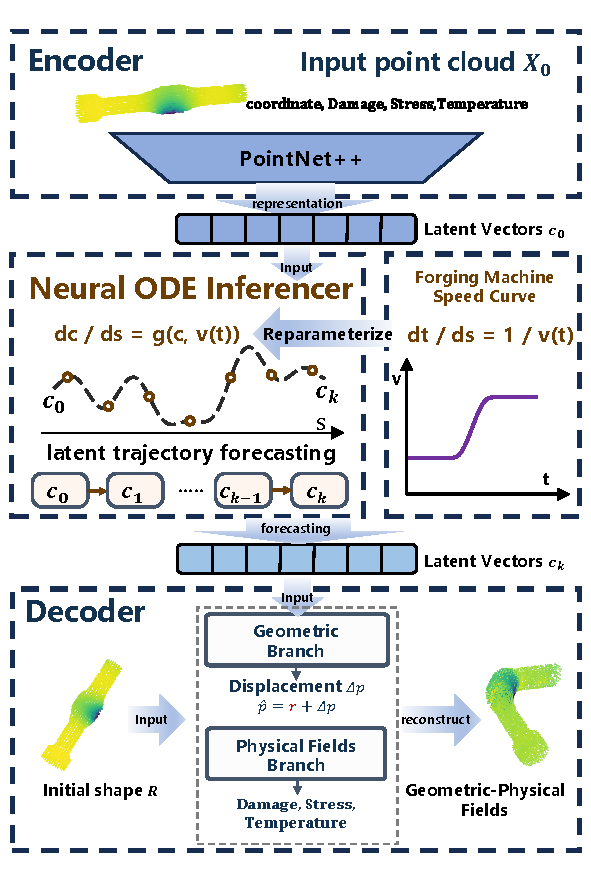
\includegraphics[width=12cm]{world_model_framework_wide.pdf}}
\caption{Overall framework of the forging world model: the encoder $E$ maps the point cloud to the latent state $c_k$, the latent dynamics model $g$ propagates the latent state along the stroke conditioned on the speed profile, and the decoder $\mathrm{Dec}$ reconstructs the geometry--multi-physics point cloud from the latent state.}
\label{fig:world_model}
\end{figure}

\subsection{Point Cloud Encoder}
Denote the point cloud of step $k$ as $X_k=\{[\,p_i;\ h_i\,]\}_{i=1}^{N}\in\mathbb{R}^{N\times 6}$, where $p_i\in\mathbb{R}^{3}$ is the absolute coordinate and $h_i=(T_i,\sigma_i,D_i)\in\mathbb{R}^{3}$ is the temperature, von Mises stress, and damage at that point, consistent with the definition in Eq.~\ref{equ:pointcloud}. The encoder builds on the hierarchical structure of PointNet++ and extracts features level by level through sampling--grouping--local aggregation.

First, farthest point sampling (FPS) selects center points deterministically by geometry. Let $S_{m-1}$ denote the set of already selected centers (initialized with $S_0$ as an arbitrary point); the $m$-th center is
\begin{equation}
p_{m}=\arg\max_{p\in\{p_i\}}\ \min_{p'\in S_{m-1}}\big\|p-p'\big\|_{2},\qquad S_{m}=S_{m-1}\cup\{p_{m}\},
\end{equation}
i.e., the point farthest from the already selected set is chosen, where $p_i$ is the coordinate of point $i$ and $S_m$ is the set of the first $m$ selected centers. This sampling is insensitive to the input order of the points. For any center point $p_i$, a ball query with radius $\delta$ obtains its local neighborhood
\begin{equation}
\Omega_i=\{\,j:\ \|p_j-p_i\|_{2}\le \delta\,\},
\end{equation}
A shared MLP is applied to each point in the neighborhood, followed by channel-wise max pooling, to obtain the local feature of the center point
\begin{equation}
f_i=\max_{j\in\Omega_i}\ \mathrm{MLP}\big([\,h_j;\ p_j-p_i\,]\big),
\end{equation}
where $f_i\in\mathbb{R}^{d_1}$ is the local feature of center $i$ ($d_1$ is the first-level feature dimension), $p_j-p_i\in\mathbb{R}^{3}$ is the coordinate of neighbor $j$ relative to the center, and $h_j\in\mathbb{R}^{3}$ is the physical-field feature of point $j$ (first layer). Repeating the above sampling--grouping--aggregation for $n_{\text{SA}}$ levels expands the receptive field from local to global.

Finally, global max pooling is applied to the last-level features followed by an MLP mapping, yielding the low-dimensional latent state that carries the state of the entire workpiece:
\begin{equation}
c_k=\mathrm{MLP}\Big(\max_{i} f_i^{(n_{\text{SA}})}\Big)\in\mathbb{R}^{d} .
\end{equation}
where $f_i^{(n_{\text{SA}})}$ is the center-point feature output by the $n_{\text{SA}}$-th (last) level, $\max_i$ denotes channel-wise max over all center points, and $d$ is the latent-state dimension. Since sampling and grouping depend only on geometric distances and the neighborhood information is aggregated by symmetric max pooling, the encoder is permutation-invariant with respect to the input order of points, i.e., $E(\Pi(X_k))=E(X_k)$ for any permutation $\Pi$.

\subsection{Latent Dynamics Model}
The conditional input of the latent dynamics model is the die speed profile $v_y(t)$, which can be any continuous curve; the curves in the training data are generated by low-dimensional parameterized sampling, covering constant-speed, fast-then-slow, slow-then-fast, and other shapes. The speed value is normalized and fed into the vector field to be learned together with the latent state.

On this basis, the latent dynamics model describes the continuous evolution of the latent state in the augmented ``physical-time--latent-state'' space: taking the stroke $s$ (the downward displacement of the press) as the integration variable, from $ds=v_y(t)\,dt$ we have
\begin{equation}
\frac{dc}{ds}=g\big(c,\,v_y(t)\big),\qquad \frac{dt}{ds}=\frac{1}{v_y(t)} ,
\end{equation}
where $c\in\mathbb{R}^{d}$ is the latent state, $g:\mathbb{R}^{d}\times\mathbb{R}\to\mathbb{R}^{d}$ is the vector field to be learned (parameterized by an MLP), and $t$ and $s$ are the physical time and stroke, respectively. The latent dynamics model thus integrates step by step along the stroke $s$, while the speed profile is given with the physical time $t$ as the independent variable; the two are converted through $ds=v_y(t)\,dt$ (equivalently $dt/ds=1/v_y(t)$), and the physical time $t$ advances synchronously with the integration as an augmented state, i.e., the integration step is taken in displacement while the speed is expressed on the time axis. The speed profile is thereby embedded as a physical prior into the time-scale transformation, aligning the prediction time scale with the true process. The latent state of two adjacent steps is obtained by integrating over the interval:
\begin{equation}
c_{k+1}=c_k+\int_{s_k}^{s_{k+1}} g\big(c(s),\,v_y(t(s))\big)\,ds ,
\end{equation}
where $s_k$ and $s_{k+1}$ are the strokes corresponding to two adjacent steps, and $c(s)$ is the latent state evolving along the stroke. This differential equation is solved by the fourth-order Runge--Kutta method, with backpropagation performed via the adjoint method. Because the latent dynamics model integrates over the stroke with the speed profile given analytically, the integration step need not coincide with the training step: training uses a fine step to constrain the local dynamics, while inference uses a coarse step to cover the entire history, with both sharing the same vector field.

\subsection{Joint Geometry--Physics Decoder}
The decoder adopts a DeepONet structure and learns an operator $\mathrm{Dec}$ mapping the latent state to a displacement--physics-field map: the branch network takes the latent state $c_k$ as input, the trunk network takes the reference coordinate $r_i$ as the query point, and after tensor fusion a shared output layer jointly produces the displacement and physical fields at that point. The overall structure of the decoder is shown in Fig.~\ref{fig:decoder}. Taking the query coordinate as the trunk input enables the decoder to query arbitrary reference points and share a spatial basis across points, so that a single network characterizes the field distribution over the entire point cloud. Let the first-step geometry be $R=\{r_i\}_{i=1}^{N}$ ($r_i\in\mathbb{R}^{3}$ is the coordinate of the $i$-th reference point), i.e., the first-step point cloud of this sample (denoted $X_0$), the initial geometry of the workpiece; it is a known input in both training and inference and varies sample by sample with the initial condition. The point-wise action of the decoder on each reference point is
\begin{equation}
\begin{aligned}
\hat{y}_i&=\big(\hat{T}_i,\ \hat{\sigma}_i,\ \hat{D}_i\big),\\
\big[\,\Delta p_i;\ \hat{y}_i\,\big]&=W\big(f_{b}(c_k)\otimes f_{t}(r_i)\big)+b,
\end{aligned}
\end{equation}
where $f_{b}:\mathbb{R}^{d}\to\mathbb{R}^{P\times C}$ and $f_{t}:\mathbb{R}^{3}\to\mathbb{R}^{P}$ are the branch and trunk networks, $P$ is the number of spatial bases, and $C=6$ is the number of output channels (3 displacement dimensions and 3 physical fields); $W\in\mathbb{R}^{C\times(PC)}$ and $b\in\mathbb{R}^{C}$ are the weight and bias of the output layer; $\Delta p_i\in\mathbb{R}^{3}$ is the displacement prediction of reference point $i$, and $\hat{T}_i$, $\hat{\sigma}_i$, $\hat{D}_i$ are the predicted temperature, von Mises stress, and damage, respectively. Let $\mathrm{Dec}(c_k)$ denote the complete point cloud generated from $c_k$; its point-wise action on any reference point $r_i$ is exactly the above equation. The displacement and physical fields are coupled from the same latent state through a shared output layer, constraining each other physically.

\begin{figure}[htbp]
\centerline{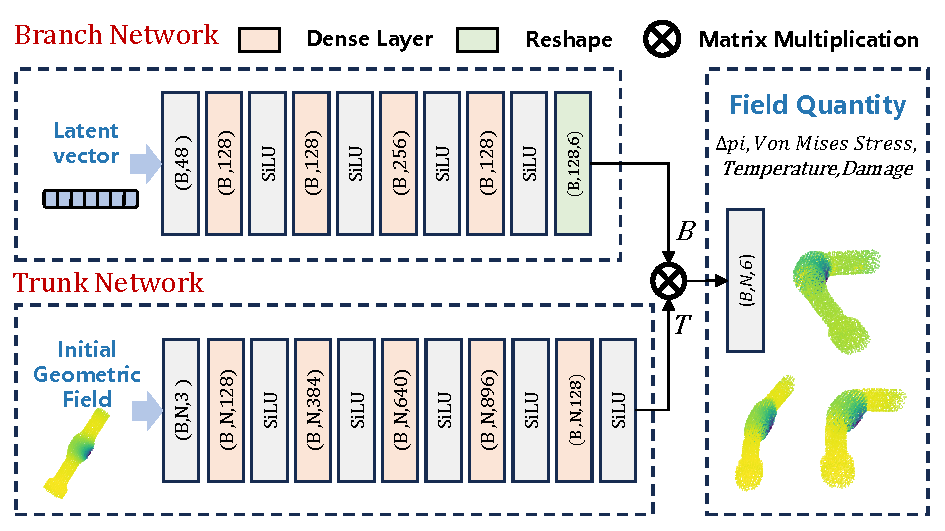
\includegraphics[width=12cm]{decoder-wide.pdf}}
\caption{Schematic of the decoder architecture.}
\label{fig:decoder}
\end{figure}

\textbf{Geometry.} With the first-step geometry $R$ as a hard baseline, the network predicts only the relative displacement:
\begin{equation}
\hat{p}_i=r_i+\Delta p_i .
\end{equation}
When there is no deformation, $\Delta p_i\approx0$, i.e., $\hat{p}_i\approx r_i$; this residual form converts ``reconstructing the geometry'' into ``learning the displacement'', which both reduces the learning difficulty and ensures that the initial shape is exactly restored.

\textbf{Physical fields.} The three physical fields are regressed using the same reference coordinate $r_i$ as the query point. Since the query coordinate always takes the reference point $r_i$ in the first-step geometry $R$ (the index is the material-point identity) during both training and inference, the input distribution of the two stages remains consistent, avoiding distribution shift caused by geometric evolution. Accordingly, geometry and physical fields are jointly output point by point from the same latent state to reconstruct the point cloud:
\begin{equation}
\hat{X}_k=\big\{\,(\hat{p}_i,\ \hat{y}_i)\,\big\}_{i=1}^{N},
\end{equation}
yielding $\hat{X}_k\in\mathbb{R}^{N\times 6}$, which jointly reconstructs the shape and multi-physics fields from the same latent state and reinforces the physical consistency between geometry and fields.

\subsection{Training Objective}
The world model is trained in two stages. In the first stage, the encoder and decoder are trained with only the reconstruction loss, so that the latent state can be reconstructed into the geometry--multi-physics point cloud. In the second stage, the latent dynamics model is trained with a latent-space prediction loss and a multi-step rollout loss to optimize its vector field, so that the latent state can be propagated autoregressively along the die speed profile.

The reconstruction loss of the first stage is the point-wise error of the point cloud reconstructed by the decoder from the true latent state, summed over all steps and averaged over the batch ($\mathbb{E}[\cdot]$ denotes the expectation over the batch):
\begin{equation}
\mathcal{L}_{\text{recon}}=\mathbb{E}\Big[\sum_{k}\big\|\mathrm{Dec}(c_k)-X_k\big\|^{2}\Big] .
\end{equation}

The latent-space prediction loss of the second stage is the mean squared error between the predicted latent state and the true encoding, where $\hat{c}_{k+1}$ is the next latent state predicted by the latent dynamics model, $c_{k+1}=E(X_{k+1})$ is the corresponding true encoding, and $\mathrm{sg}(\cdot)$ is the stop-gradient operator (cutting off gradient backpropagation to the encoder):
\begin{equation}
\mathcal{L}_{\text{pred}}=\mathbb{E}\Big[\big\|\hat{c}_{k+1}-\mathrm{sg}(c_{k+1})\big\|^{2}\Big] .
\end{equation}

The multi-step rollout loss enhances long-horizon prediction stability and is combined with the prediction loss via weight $\beta_M$: starting from step $k$, an $M$-step autoregressive rollout is performed, where each step advances from the latent state predicted at the previous step rather than using the true encoding, and the loss is computed between the predicted latent state at each step on the rollout path and the true encoding of that step:
\begin{equation}
\mathcal{L}_{\text{rollout}}=\mathbb{E}\Big[\sum_{k}\sum_{j=1}^{M}\big\|\hat{c}_{k}^{(j)}-\mathrm{sg}(c_{k+j})\big\|^{2}\Big],
\end{equation}
where the autoregressive rollout is
\begin{equation}
\begin{aligned}
\hat{c}_{k}^{(0)} &= \mathrm{sg}(c_k), \\
\hat{c}_{k}^{(j+1)} &= \hat{c}_{k}^{(j)}+\int_{s_{k+j}}^{s_{k+j+1}} g\big(\hat{c}_{k}^{(j)},\,v_y(t(s))\big)\,ds ,
\end{aligned}
\end{equation}
$\hat{c}_{k}^{(j)}$ is the predicted latent state after rolling out $j$ steps from step $k$, and $c_{k+j}=E(X_{k+j})$ is the true encoding of the corresponding step; the prediction at each step on the rollout path is directly supervised by the true encoding of that step.

  \section{Forging Optimization Control}
\label{sec:control}

This section builds a continuous speed-profile policy on top of the world model in Section \ref{sec:world_model}. With the world model as a propagatable environment, the policy performs stepwise decision-making conditioned on the latent state inside the world model to generate the entire continuous speed profile, which is then deployed to the equipment once; training is conducted entirely within the world model without interacting with the real equipment. The overall pipeline is shown in Fig.~\ref{fig:control}.

\begin{figure}[htbp]
\centerline{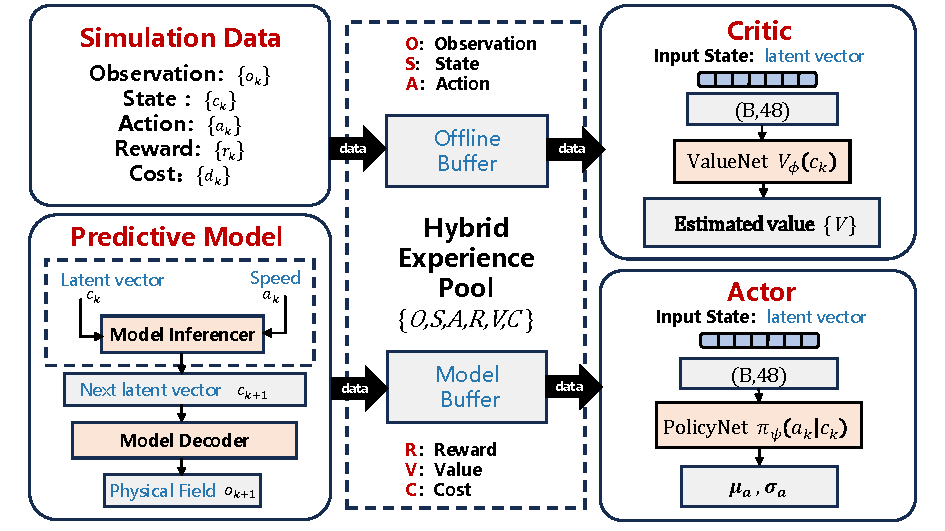
\includegraphics[width=12cm]{control-1-wide.pdf}}
\caption{Schematic of policy training.}
\label{fig:control}
\end{figure}

\subsection{Decision Problem Formulation within the World Model}
The die-speed decision is formulated as a finite-horizon constrained Markov decision process (CMDP) with safety constraints~\cite{altman2021constrained}. This process is defined only within the world model and is used for offline policy training: the state transition is provided by the world model, and the entire training does not interact with the equipment; after training, the complete speed profile is deployed once and executed. The process is defined by five elements---state, action, transition, reward, and cost---and the objective is to maximize the cumulative reward subject to the cumulative cost constraints. Each element is defined below.

\textbf{State.} The latent state $c_k\in\mathbb{R}^{d}$ inside the world model serves as the state, and both the policy and the value function take the latent state $c_k$ as input. The decoded geometry--multi-physics point cloud (i.e., the reconstructed point cloud $\hat{X}_k$ in Section \ref{sec:world_model}) $o_k=\mathrm{Dec}(c_k)\in\mathbb{R}^{N\times 6}$ ($o_k$ is a deterministic function of $c_k$) is used only to compute the reward and cost during training and does not participate in decision-making.

\textbf{Action.} The policy determines the die speed step by step along the stroke: at step $k$, at the cumulative stroke (displacement) $s_k$, it outputs the speed of that step $v_k=a_k\in\mathbb{R}$, bounded by the equipment capability, $v_k\in[v_{\min},v_{\max}]$. The per-step speeds constitute the speed profile $v(s)$ with the stroke as the independent variable; then, via $dt=ds/v(s)$, the independent variable is converted from displacement $s$ to time $t$, yielding the speed profile with time as the independent variable
\begin{equation}
v_y(t)=v\big(s(t)\big),
\end{equation}
where $s(t)$ is the cumulative stroke as a function of time, obtained by integrating the above and monotonically increasing. This profile $v_y(t)$ is the speed--time command directly executable by the press and the reference for efficiency metrics such as forging time.

\textbf{Transition.} $c_{k+1}=c_k+\int_{s_k}^{s_{k+1}}g\big(c,v_y(t)\big)\,ds$: the latent state is propagated by integrating along the stroke over the $k$-th stroke segment $[s_k,s_{k+1}]$ according to $v(s)$.

\textbf{Stroke constraint.} The total stroke satisfies
\begin{equation}
\int_{0}^{t_f}v_y(t)\,dt=\Delta h .
\end{equation}
The duration of each segment is determined by the speed of that step, $\Delta t_k=\int_{s_k}^{s_{k+1}}ds/v(s)$: the higher the speed, the shorter the segment duration.

\textbf{Reward.} The reward balances efficiency and quality step by step. At step $k$, the world model decodes the stress field $\{\hat{\sigma}_i\}_{i=1}^{N}$, which is sorted in descending order, with the top $m$ values denoted $\hat{\sigma}_{(1)}\ge\hat{\sigma}_{(2)}\ge\cdots\ge\hat{\sigma}_{(m)}$. Then define
\begin{equation}
\bar{\sigma}_k=\frac{1}{m}\sum_{j=1}^{m}\hat{\sigma}_{(j)},\qquad
u_k=\frac{\mathrm{std}(\hat{\sigma}_i)}{\mathrm{mean}(\hat{\sigma}_i)},
\end{equation}
where $\bar{\sigma}_k$ characterizes the magnitude of the field stress level, and $u_k$ is the coefficient of variation of the stress field, characterizing the degree of stress concentration. The reward is defined as
\begin{equation}
r_k=w_1 e^{-\Delta t_k}-w_2\,\bar{\sigma}_k-w_3\,u_k,
\end{equation}
where $\Delta t_k$ is the duration of the $k$-th segment, and $w_1$, $w_2$, $w_3$ are weighting coefficients. The higher and more non-uniform the stress level, the faster the damage evolution; the reward penalizes these two terms, guiding the policy to shorten the forging time while keeping the workpiece in a low and uniform stress state, forming a complement between soft guidance and the hard damage constraint.

\textbf{Cost.} The cost characterizes the stepwise damage violation:
\begin{equation}
d_k=\mathrm{relu}(D_k-D_{\text{cr}}),
\end{equation}
where $D_k$ is the maximum accumulated damage of the workpiece at step $k$, i.e., the maximum of the damage field at that step, corresponding to the value of $D(t)$ in Eq.~\ref{equ:model} at step $k$; $D_{\text{cr}}$ is the critical damage value, and $d_k=0$ indicates no violation at that step.

\textbf{Optimization objective.} Maximize the cumulative reward while satisfying the damage constraint at every step:
\begin{equation}
\max_{\psi}\ \mathbb{E}\Big[\sum_{k}\gamma^{k} r_k\Big]\quad \text{s.t.}\quad \mathbb{E}[d_k]\le 0,\quad \forall k,
\end{equation}
where $\gamma$ is the discount factor. The constraint is stepwise, i.e., the accumulated damage must not exceed the critical value at every step ($D_k\le D_{\text{cr}}$).

\subsection{Continuous Representation of the Action}
The die speed is given continuously with the stroke as the independent variable and is differentiable along the stroke, so the speed profile $v_y(t)$ is smooth with no acceleration jumps and can be directly substituted into the stroke integral $\frac{dc}{ds}=g(c,\,v_y(t))$ of the latent dynamics model; the change of the single-step speed is thus smoothly distributed along the stroke without high-frequency jitter. The stroke equality holds automatically by the definition in the displacement domain, and the speed bounds and the damage constraint only delimit the feasible region without compressing the decision freedom.
% 【实验章待补：动作参数化消融——样条插值 vs 折线直连】

\subsection{Policy and Optimization Algorithm}
The policy is a Gaussian distribution conditioned on the latent state, outputting a normal distribution over the speed control at each step:
\begin{equation}
\begin{aligned}
\pi_{\psi}(a_k\mid c_k)&=\mathcal{N}\big(a_k;\ \mu_{\psi}(c_k),\ \sigma_{\psi}^{2}(c_k)\big),\\
a_k&=\mu_{\psi}(c_k)+\sigma_{\psi}(c_k)\odot\varepsilon,\quad \varepsilon\sim\mathcal{N}(0,I),
\end{aligned}
\end{equation}
where $\mu_{\psi}(c_k)\in\mathbb{R}$ and $\sigma_{\psi}(c_k)\in\mathbb{R}_{>0}$ are the mean and standard deviation output by the policy network $\pi_{\psi}:\mathbb{R}^{d}\to\mathbb{R}^{2}$, $\odot$ denotes element-wise multiplication, $a_k=v_k\in\mathbb{R}$ is the speed control at step $k$, and the variance is diagonal; at solving (inference) time the mean $\mu_{\psi}(c_k)$ is taken as the deterministic output (the policy network is a small MLP acting on the latent state).

Offline safe reinforcement learning is adopted to solve this CMDP: the stepwise constraint is converted into an unconstrained form via Lagrangian relaxation, defining a constraint-aware single-step reward
\begin{equation}
\tilde r_k=r_k-\lambda\,d_k,
\end{equation}
where $r_k$ is the reward at step $k$, $d_k$ is the damage violation at step $k$, and $\lambda$ is the dual variable. The Lagrangian function is constructed as
\begin{equation}
\mathcal{L}(\psi,\lambda)=\mathbb{E}\Big[\sum_{k}\gamma^{k}\ln \pi_{\psi}(a_k\mid c_k)\cdot A(c_k,a_k)\Big],
\end{equation}
where the stepwise advantage function is
\begin{equation}
A(c_k,a_k)=\tilde r_k+\gamma\hat{V}(c_{k+1})-\hat{V}(c_k),
\end{equation}
and $\hat{V}(c_k)$ is the value estimate (critic), whose network parameters are denoted $\phi$. The value network is trained by minimizing the one-step temporal-difference (TD) error, with the target side stopped-gradient:
\begin{equation}
\mathcal{L}_{V}(\phi)=\mathbb{E}\Big[\big(\hat{V}(c_k)-\big[\tilde r_k+\gamma\,\mathrm{sg}(\hat{V}(c_{k+1}))\big]\big)^{2}\Big],
\end{equation}
where $\mathrm{sg}(\cdot)$ is the stop-gradient operator. To encourage exploration and prevent premature convergence, a stepwise entropy regularization term is added. Furthermore, the ``slow-then-fast'' shape of the die speed has a clear motivation for damage control~\cite{bambach2018towards}: at the early stage of deformation the contact impact and local stress concentration make damage initiation most sensitive, so a low speed suppresses damage accumulation, and after the material softens sufficiently the speed is increased to shorten the high-temperature dwell. This work does not follow that prior work in hard-coding the prior into a parameterized curve family; instead, it is reduced to a soft preference via a monotonicity regularization term:
\begin{equation}
\mathcal{R}_{\text{mono}}(\psi)=\mathbb{E}\Big[\sum_{k}\gamma^{k}\,\max\big(0,\,v_k-v_{k+1}\big)\Big],
\end{equation}
This regularization is positive only when $v_k>v_{k+1}$ (the current step is faster than the next, i.e., decelerating) and zero otherwise, so it penalizes only the deceleration segments and induces a monotonically non-decreasing speed; it has no preference over the acceleration magnitude and thus does not restrict the policy's ability to represent any speed profile. Incorporating the entropy regularization and the monotonicity regularization into the objective yields
\begin{equation}
\begin{aligned}
\mathcal{J}(\psi,\lambda)=&\,\mathcal{L}(\psi,\lambda)+\eta\,\mathbb{E}\Big[\sum_{k}\gamma^{k}H\big[\pi_{\psi}(\cdot\mid c_k)\big]\Big]\\
&-\lambda_m\,\mathcal{R}_{\text{mono}}(\psi),
\end{aligned}
\end{equation}
where $\eta$ and $\lambda_m$ are the entropy coefficient and the monotonicity regularization strength, respectively, and $H[\cdot]$ is the policy entropy.

The optimization adopts dual gradient ascent: first fix $\lambda$ and maximize $\mathcal{J}$ with respect to $\psi$ to update the policy parameters; then fix $\psi$ and update the dual variable according to the degree of constraint violation
\begin{equation}
\lambda\leftarrow\max\big(0,\ \lambda+\alpha_{\lambda}\bar{d}\big),\qquad \bar{d}=\max_{k}\,(D_k-D_{\text{cr}}),
\end{equation}
where $\alpha_{\lambda}$ is the dual step size, and $\bar{d}$ is the maximum (signed) difference between the damage and the critical value over all steps along the entire trajectory. When a violation step exists ($\bar{d}>0$), $\lambda$ increases to strengthen the penalty; when every step is below the critical value ($\bar{d}<0$), $\lambda$ decreases to relax the constraint. The policy training collects experience via closed-loop rollout within the world model: at each step the speed $v_k$ is output conditioned on the latent state $c_k$, and the state is advanced autoregressively by the world model as $c_{k+1}=c_k+\int_{s_k}^{s_{k+1}}g(c,v_y(t))\,ds$, isomorphic to the solving stage; the whole process is offline and requires no interaction with the real equipment. Training uses a mixed experience replay buffer, where the transition samples come from the finite-element simulation dataset $\mathcal{B}$ and the data generated by world-model propagation; $\rho$ is the proportion of simulation data in a batch, and the two kinds of samples are mixed according to this proportion to jointly participate in the update.

\subsection{Decision Solving and Execution}
In the solving stage, the policy performs stepwise rollout decision-making within the world model: at step $k$, the speed $v_k$ is output conditioned on the latent state $c_k$; after obtaining the per-step speeds, the entire profile $v_y(t)$ is assembled. In the execution stage, this profile is deployed to the equipment once, and the equipment provides no online feedback. Compared with the single-shot parametric policy that outputs $\theta$ once and generates the entire profile in a feedforward manner, the stepwise decision-making of this work can exploit the evolution information of damage, stress, and other quantities step by step and adapt to different initial temperature fields.

  \section{Experiment}
\subsection{Dataset and Setup}
This work targets the 6082 aluminum alloy control-arm forging and constructs a dataset of 600 forging simulations based on DEFORM-3D, in which both the initial temperature field and the forging speed vary, and each sequence contains 67 deformation steps. Ten non-uniform initial temperature fields are obtained by simulating the cooling process. Each simulation outputs multi-physics fields such as temperature, von Mises stress, and damage, which are stored as point clouds with about 5000 points per step, each point recording its coordinate $(x,y,z)$ and the corresponding physical quantities; the dataset is split into training, validation, and test sets.
% 【待定：训练/验证/测试划分比例】

For preprocessing, the absolute coordinates of all points are normalized along the three axes with a shared scale to preserve the workpiece shape.

The main hyperparameters are set as follows: number of points per step $N=5000$, latent-state dimension $d=48$, and encoder level count $n_{\text{SA}}=4$. The critical damage value of the damage constraint is set to $D_{\text{cr}}=0.43$.
% 【待补：其余超参数与实验环境】

\subsection{World Model Evaluation}

The world model is trained in two stages. Fig.~\ref{fig:train_loss} shows the training loss curves of the two stages: the first stage trains the encoder and decoder with the reconstruction loss (Fig.~\ref{fig:train_loss_a}), and the second stage trains the latent dynamics model with the prediction loss (Fig.~\ref{fig:train_loss_b}). The training and validation losses of both stages decrease and stabilize over epochs, converging synchronously with a stable gap and no evident overfitting, indicating that both the reconstruction representation and the latent-space dynamics have effectively converged.

\begin{figure}[H]
    \centering
    \subfloat[Stage 1 (reconstruction)]{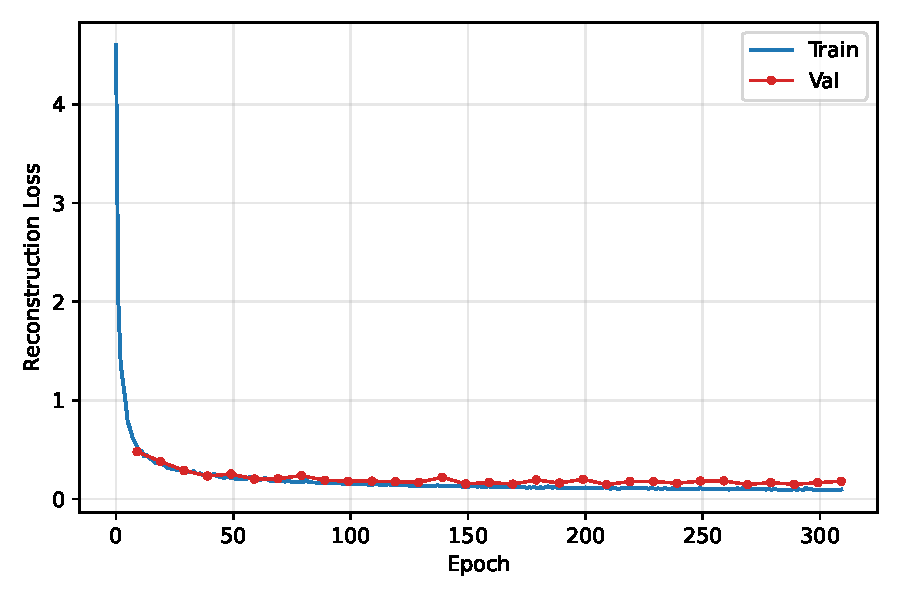
\includegraphics[width=0.44\linewidth]{train_loss_1.pdf}\label{fig:train_loss_a}}
    \qquad
    \subfloat[Stage 2 (prediction)]{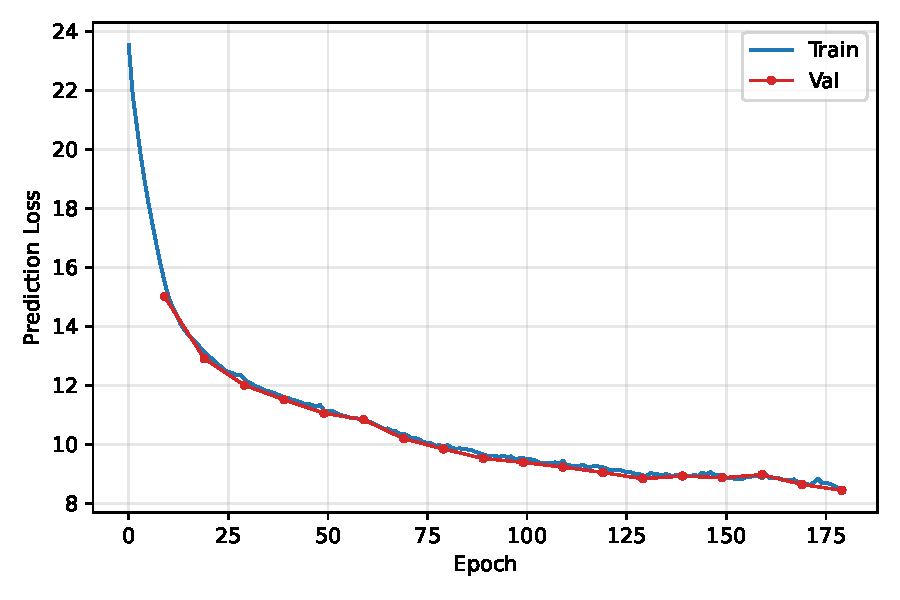
\includegraphics[width=0.44\linewidth]{train_loss_2.pdf}\label{fig:train_loss_b}}
    \caption{Loss curves of the two-stage training of the world model.}
    \label{fig:train_loss}
\end{figure}

To evaluate the prediction accuracy of the world model, taking the stress field as an example, its predictions are compared with the finite element (FE) simulation and the baseline method. Fig.~\ref{fig:model_result} shows the stress-field point clouds at five deformation steps along the deformation history: the first row is the FE ground truth, the second row is the prediction of the proposed model, and the third row is the result of the DeepONet baseline. The stress distribution of the proposed model is highly consistent with the ground truth, with the deviation concentrated in local regions and of small magnitude; the baseline exhibits a clear distribution shift in the stress-concentration regions.

\begin{figure}[H]
\centerline{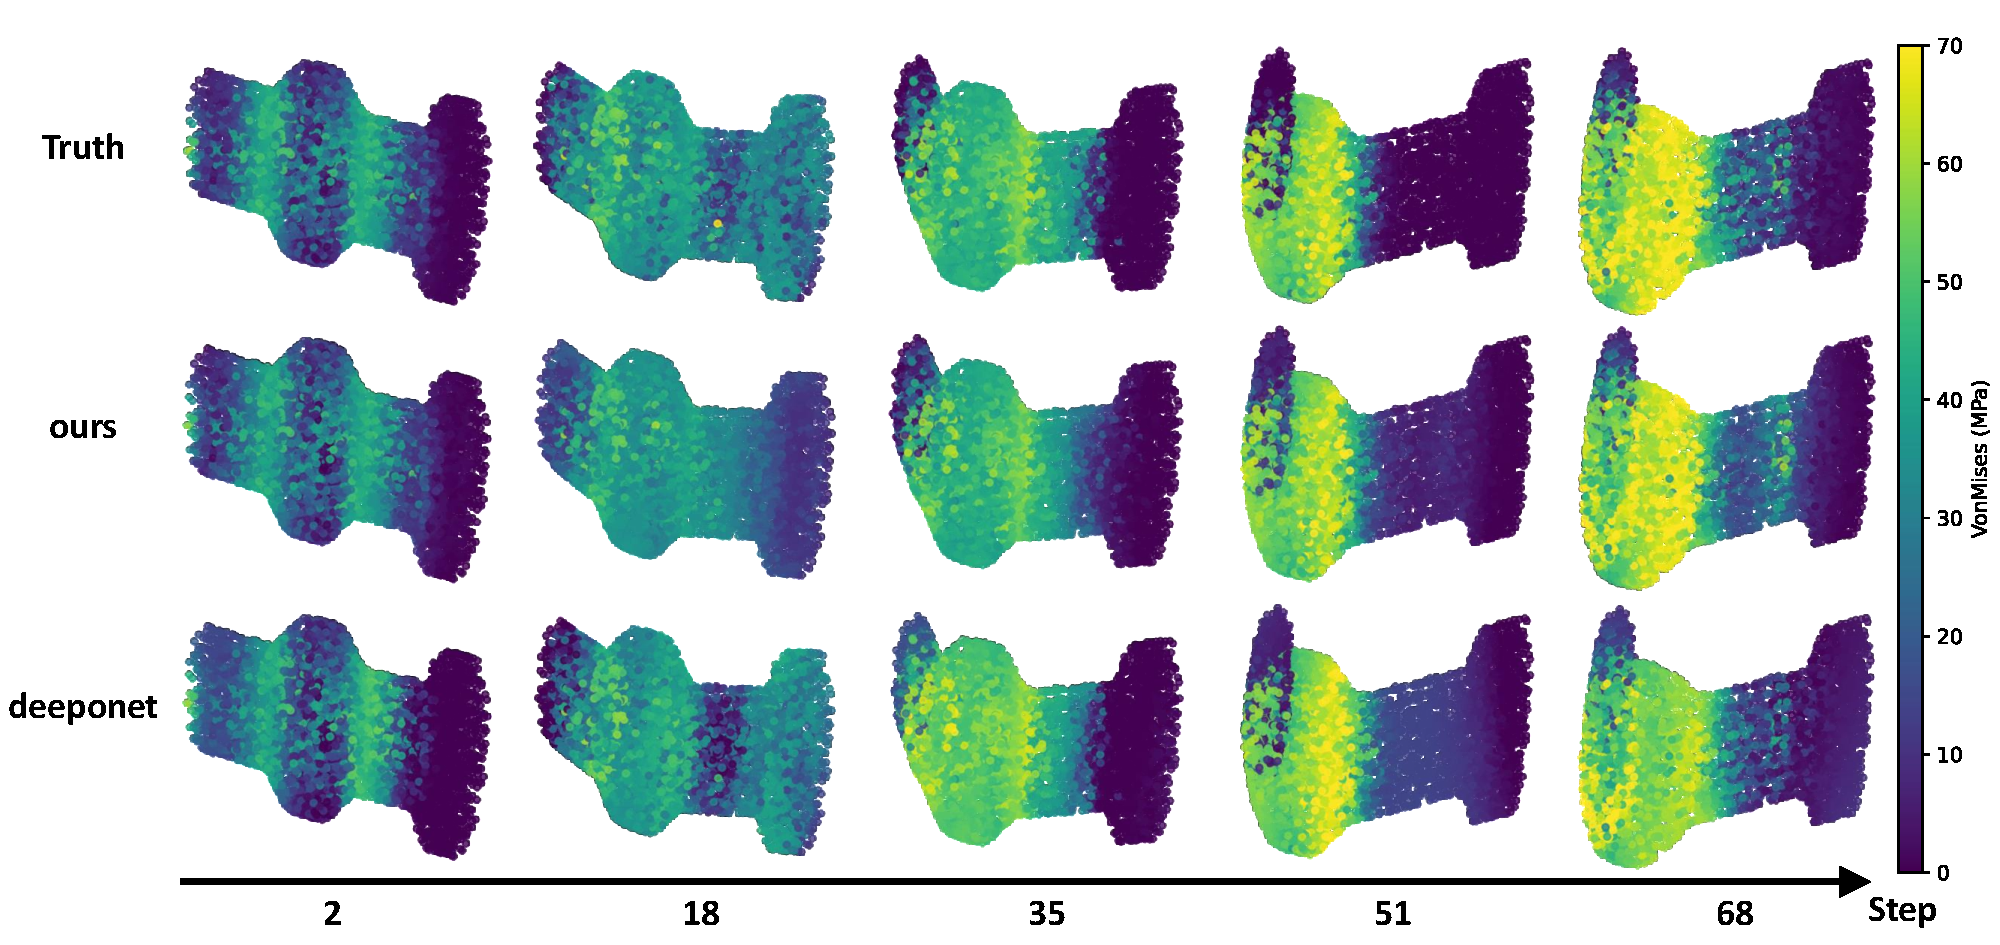
\includegraphics[width=9cm]{timeline-1.pdf}}
\caption{Stress-field prediction comparison: the three rows, from top to bottom, are the FE ground truth, the prediction of the proposed model, and the DeepONet baseline; each row shows the point clouds at five deformation steps along the deformation history from left to right.}
\label{fig:model_result}
\end{figure}

Errors are further quantified on the test set. At inference, the trained latent dynamics model integrates along the stroke to propagate, and the decoder reconstructs the point cloud. The geometry error is reported as per-axis root mean square error (RMSE) in mm, and the physical-field errors are normalized by the mean and variance of each field on the training set, computed per channel and then averaged, with the errors compared pointwise with the corresponding FE results. Under this rollout manner, the per-axis geometry RMSE is 1.63 mm, and the averaged normalized MSE over the three physical fields is 0.080; the per-channel results are shown in Table~\ref{tab:model_error}. Among the three channels, the von Mises stress has the highest normalized error, followed by temperature and then damage. The von Mises stress is jointly determined by the strain rate and temperature and depends on the entire deformation history, making it the most sensitive to process conditions among the three fields; temperature is dominated by heat conduction with a smooth distribution and is relatively easier to fit; damage accumulates only locally with most points close to zero, so the pointwise error is diluted by a large number of near-zero points and its normalized error is the lowest. The decision stage requires repeatedly rolling out the entire curve within the world model, thereby supporting stepwise decision-making.

\begin{table}[H]
\centering
\caption{Prediction errors of the proposed and baseline methods}
\label{tab:model_error}
\setlength{\tabcolsep}{5pt}
\footnotesize
\begin{tabular}{l c c c c c}
\toprule
 & RMSE (mm) & \multicolumn{4}{c}{Normalized MSE} \\
Model & Geometry & Temp. & von Mises & Dmg. & avg. \\
\midrule
Ours & 1.63 & 0.104 & 0.115 & 0.022 & 0.080 \\
DeepONet (no latent) & 1.57 & 0.129 & 0.255 & 0.031 & 0.138 \\
\bottomrule
\end{tabular}

\vspace{2pt}
{\footnotesize Note: geometry is per-axis RMSE (mm); field normalized MSE uses training-set statistics; avg.\ is the mean over the three field channels; all metrics are averaged over the test-set rollout. Full-model physical RMSE: 8.8\,$^{\circ}$C, 6.3 MPa, $4.7\times10^{-3}$ (temperature, von Mises, damage).}
\end{table}

The same-metric errors on the training set are 1.87 mm for geometry, 9.7\,$^{\circ}$C for temperature, 7.9 MPa for von Mises stress, and $5.6\times10^{-3}$ for damage, slightly higher than on the test set. The reason is that the training set covers a wider range of temperature and deformation, and the normalization statistics are taken from the training set; the errors of the two sets are of the same order and the deviations of each channel are in the same direction, with no overfitting sign that the training set is significantly better than the test set.




\subsection{Decision Results}
The average reward and damage during the training of the policy are shown in Fig.~\ref{fig:combined_curves}. The average reward rises from initial fluctuations and stabilizes at a positive value (Fig.~\ref{fig:reward_a}), indicating that the policy has converged; Fig.~\ref{fig:damage_b} shows the maximum damage over the whole process in each epoch, which stabilizes below the critical value $D_{\text{cr}}$ in the late training stage. Since the maximum has not exceeded the limit, no step has exceeded the limit, and the stepwise constraint is thereby satisfied. These results show that the proposed decision method shortens the forging time while satisfying the damage constraint.

\begin{figure}[H]
    \centering
    \subfloat[Reward]{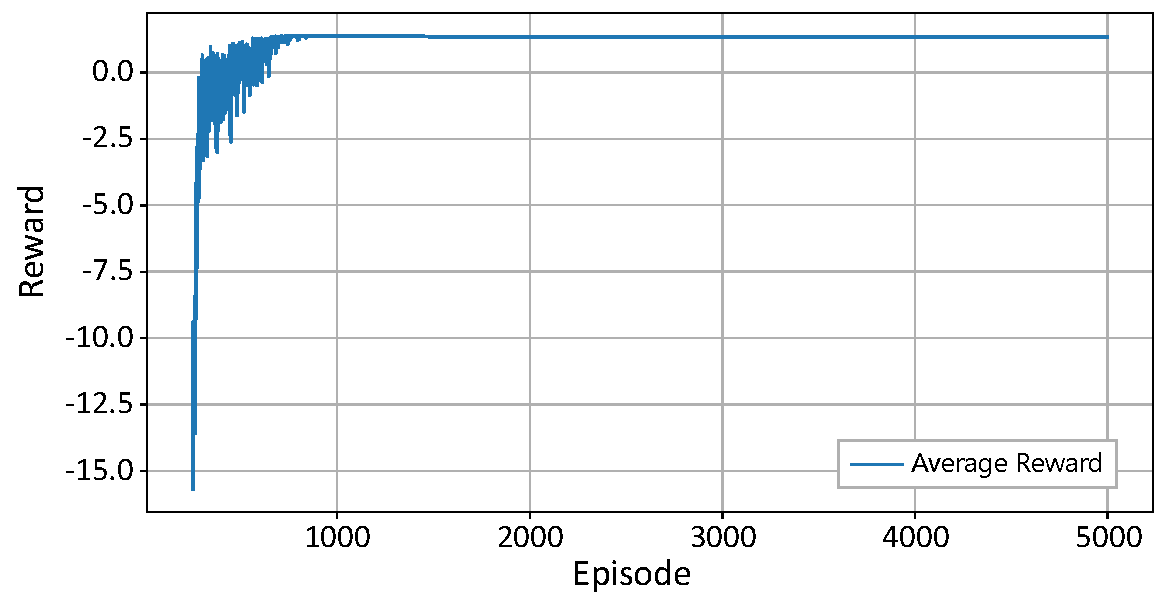
\includegraphics[width=0.38\linewidth]{reward-1.pdf}\label{fig:reward_a}}
    \qquad
    \subfloat[Damage]{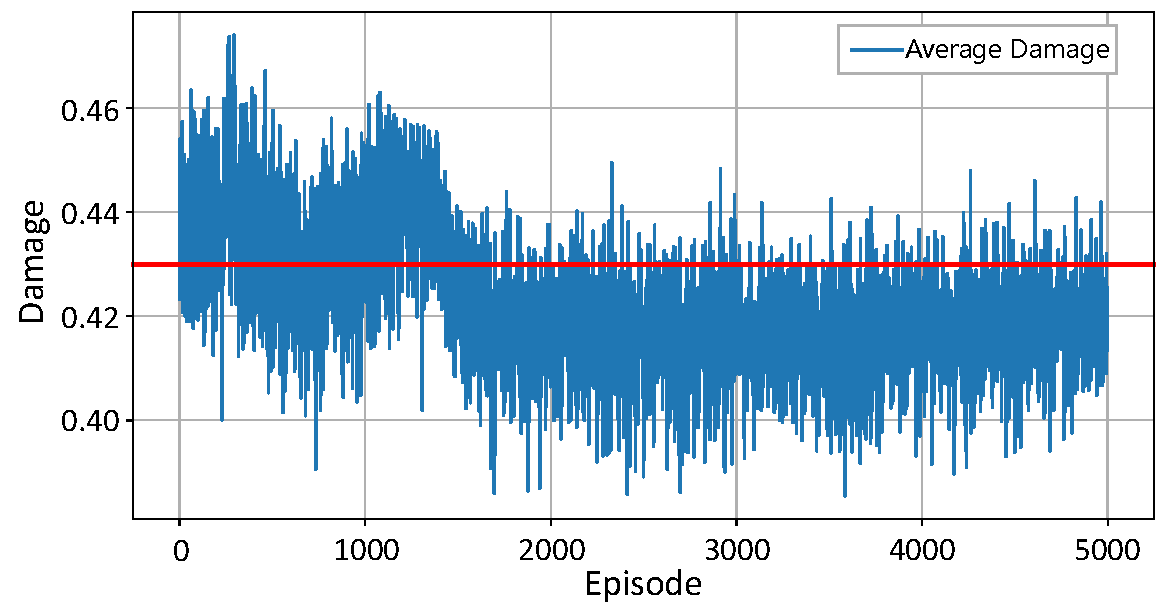
\includegraphics[width=0.38\linewidth]{damage-1.pdf}\label{fig:damage_b}}
    \caption{Training parameter over epochs.}
    \label{fig:combined_curves}
\end{figure}

Fig.~\ref{fig:ours_speed} shows the speed profiles and damage curves generated by the proposed method under different initial temperature fields. When the initial temperature rises from $474\,^{\circ}\mathrm{C}$ to $500\,^{\circ}\mathrm{C}$, the acceleration segment of the speed profile advances and the forging time shortens, indicating that the policy can adaptively adjust the speed profile according to the initial temperature field to exploit the high-temperature softening of the material; the damage curve rises gradually with deformation and reaches its peak at the last step, with its ratio to the critical damage value $D_{\text{cr}}$ still below 1.0, indicating that the damage is overall controlled.

\begin{figure}[H]
    \centering
    \begin{minipage}[t]{0.44\textwidth}
        \centering
        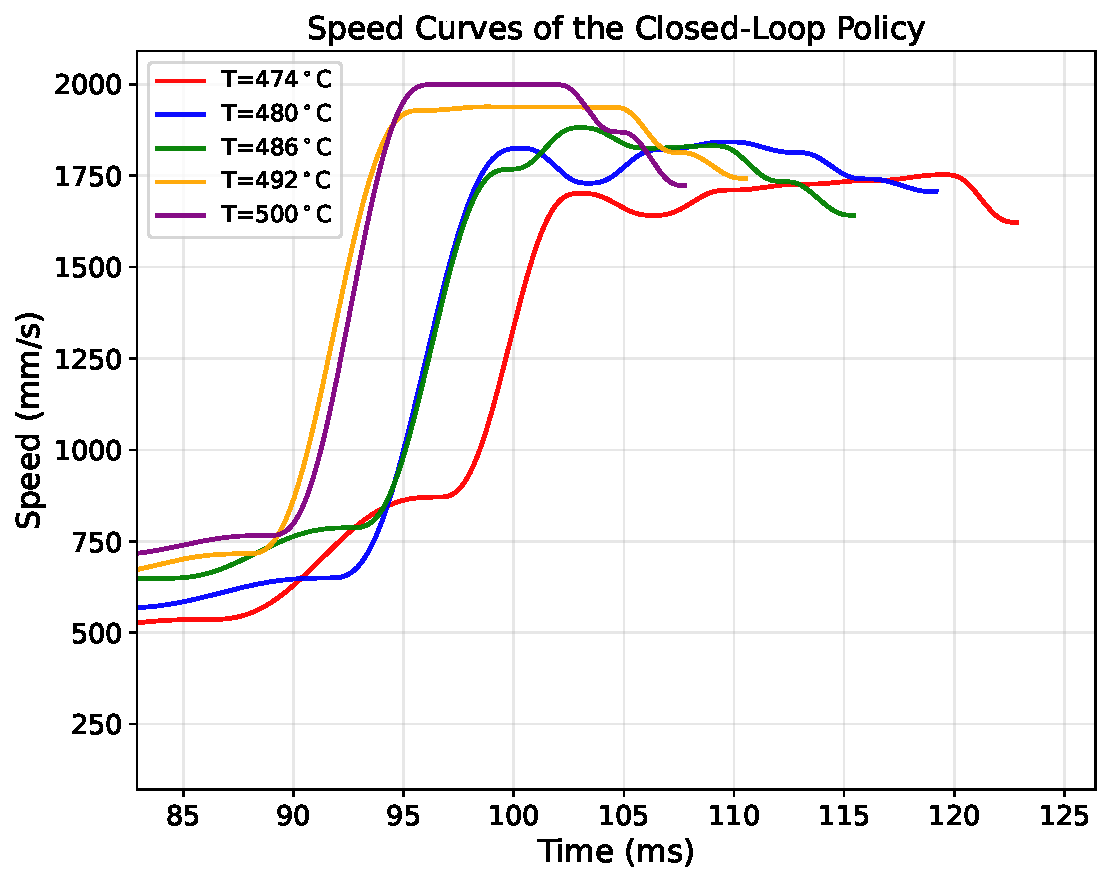
\includegraphics[width=\linewidth]{speed_close.pdf}
        \caption{Speed profiles and damage curves generated by the proposed method under different initial temperature fields ($474\,^{\circ}\mathrm{C}$--$500\,^{\circ}\mathrm{C}$). The damage curve takes the average of the top 50 points with the largest damage in the point cloud at each step.}
        \label{fig:ours_speed}
    \end{minipage}
    \qquad
    \begin{minipage}[t]{0.44\textwidth}
        \centering
        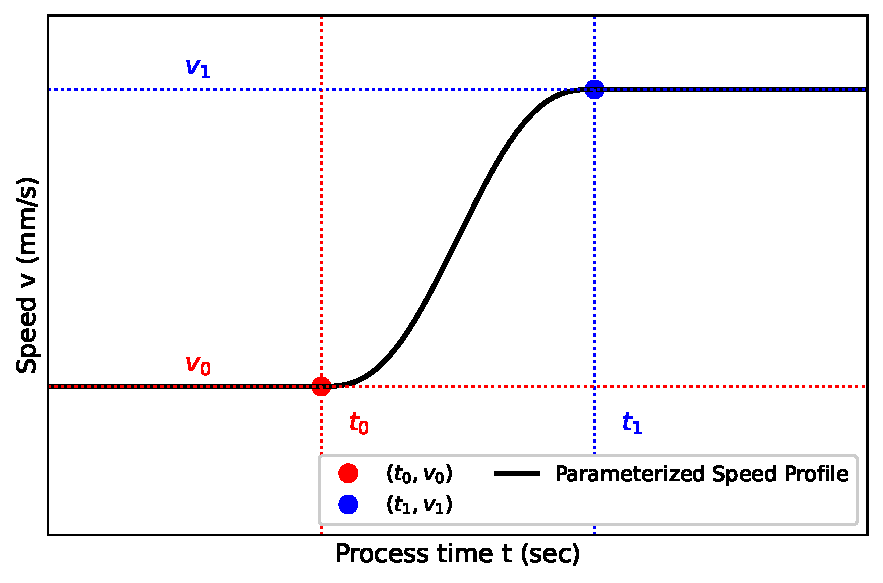
\includegraphics[width=\linewidth]{velocity_profile.pdf}
        \caption{Three-segment shape of the single-shot parametric decision.}
        \label{fig:speed_profile}
    \end{minipage}
\end{figure}

\textbf{Baselines.} The single-shot parametric decision is also a trained parametric policy; its difference from the proposed policy lies in the decision representation: the proposed method outputs the speed of each step step by step, whereas it directly gives a four-dimensional speed parameter $\theta=\{v_0,v_1,t_0,t_1\}$ in a single-shot manner and then reconstructs the entire speed profile from it. The profile is restricted to a ``constant--accelerating--constant'' three-segment shape, given by a smooth four-parameter function:
\begin{equation}
v_{y}(t)=\begin{cases}
v_{0}, & t<t_{0} \\
v_{0}+(v_{1}-v_{0})\,\xi^{3}\,(10-15\xi+6\xi^{2}), & t_{0}\le t\le t_{1} \\
v_{1}, & t>t_{1}
\end{cases}
\end{equation}
where $\xi=(t-t_0)/(t_1-t_0)$, and the components of $\theta$ correspond to the initial speed, the target speed, and the start/end instants of acceleration; this function has second-order continuous derivatives at $t_0$ and $t_1$, ensuring smooth acceleration. The parametric policy takes the initial temperature field as input and outputs $\theta$ in a single shot, with the training objective likewise being to shorten the forging time within the world model while satisfying the damage constraint. Because it does not require stepwise autoregressive generation of the curve, its decision time is lower than that of the proposed method, at the cost of forgoing the stepwise utilization of the evolution process. PSO, in contrast, is not trained; it performs a global search with particle swarm over the same parameter curve, and its decision time mainly comes from repeated fitness evaluations.

\begin{figure}[H]
    \centering
    \subfloat[Single-shot parametric decision]{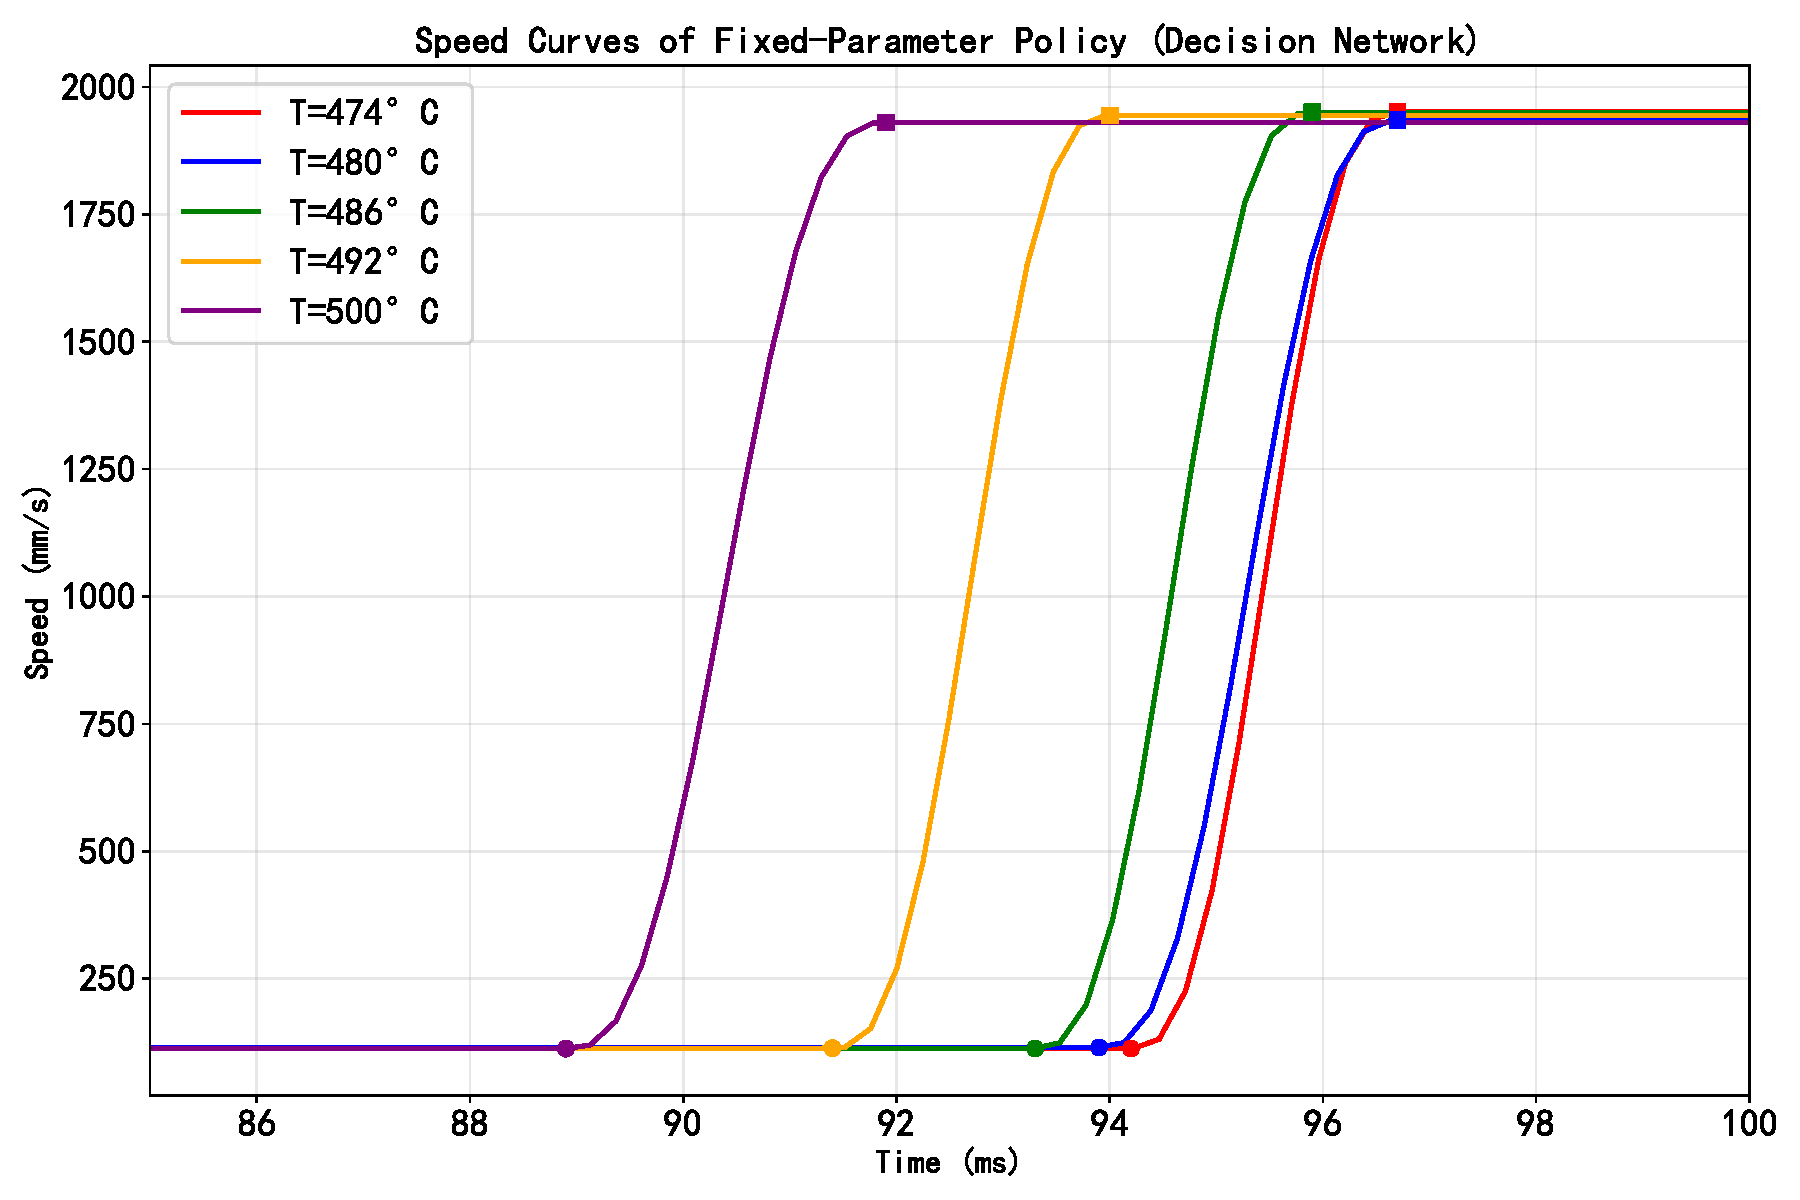
\includegraphics[width=0.40\linewidth]{NetworkSpeed_decision.pdf}\label{fig:policynet_speed}}
    \qquad
    \subfloat[PSO]{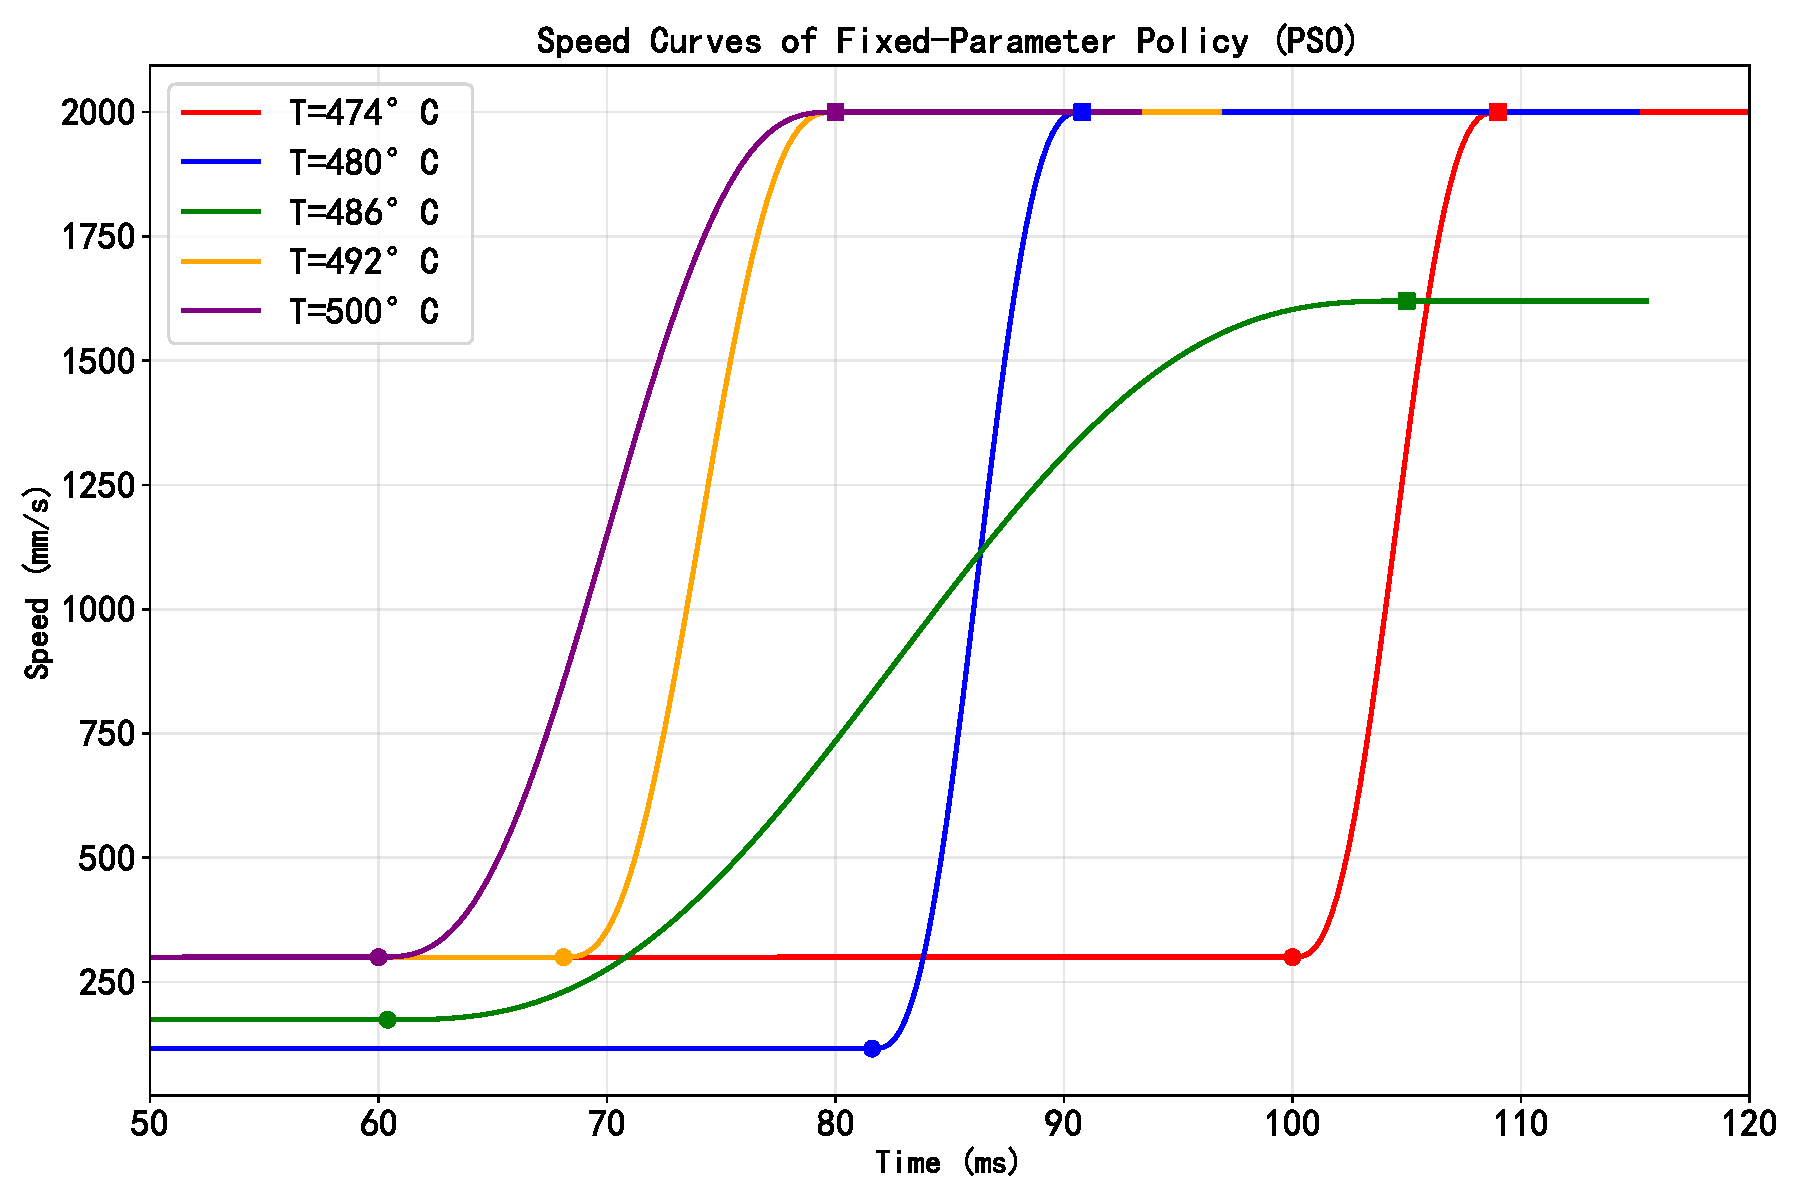
\includegraphics[width=0.40\linewidth]{NetworkSpeed_PSO.pdf}\label{fig:pso_speed}}
    \caption{Speed-profile comparison with other decision methods ($474\,^{\circ}\mathrm{C}$--$500\,^{\circ}\mathrm{C}$).}
    \label{fig:other_speed}
\end{figure}

The process performance and decision efficiency of different decision methods are further compared; the speed profiles of each method are shown in Fig.~\ref{fig:ours_speed} and Fig.~\ref{fig:other_speed}, respectively, and the quantitative results are given in Table~\ref{tab:Method Comparison}. PSO achieves the best process quality, with the shortest forging time and a damage rate of 0, but its solution is time-consuming and cannot meet the requirement of rapid pre-production decision; the single-shot parametric decision has the longest forging time and gives the decision very fast, but damage appears in the simulation and safety cannot be guaranteed; the forging time of the proposed method lies in between, slightly longer than PSO but shorter than the single-shot parametric decision. Its decision is slightly slower than the single-shot parametric decision due to autoregressive stepwise inference, yet still clearly faster than PSO, and no damage appears in the simulation test. It can be seen that the proposed method obtains damage-free safety at a very small cost in forging time, while its forging time is better than the single-shot parametric decision and its decision speed is far better than PSO.

\begin{table}[H]
\centering
\caption{Performance comparison of the three decision methods}
\setlength{\tabcolsep}{3.5pt}
\begin{tabular}{c c c c}
\toprule
\textbf{Method} & \textbf{Forge Time} & \textbf{Decision Time} & \textbf{Damage Rate}\\
& (mean$\pm$std,ms) & (mean$\pm$std,ms) & (\%)\\
\midrule
Ours & 115.14$\pm$6.15 & 105.21$\pm$4.13 & 0.00 \\
Parametric decision & 119.18$\pm$4.84 & 97.37$\pm$3.86 & 8.00 \\
PSO        & 108.72$\pm$11.55 & 2580$\pm$1370 & 0.00 \\
\bottomrule
\end{tabular}
\label{tab:Method Comparison}
\end{table}

The decision time of PSO mainly comes from repeated fitness evaluations. Fig.~\ref{fig:pso_objective} shows the convergence process of its objective function: PSO requires about 0.9 s to optimize to an objective value comparable to the parametric-policy output, and full convergence requires 2580 ms; in contrast, the parametric policy directly gives the speed parameter through a single forward inference without iterative search. Therefore, although the parametric policy does not obtain the optimal solution of PSO, it is significantly superior in time efficiency.

\begin{figure}[H]
\centerline{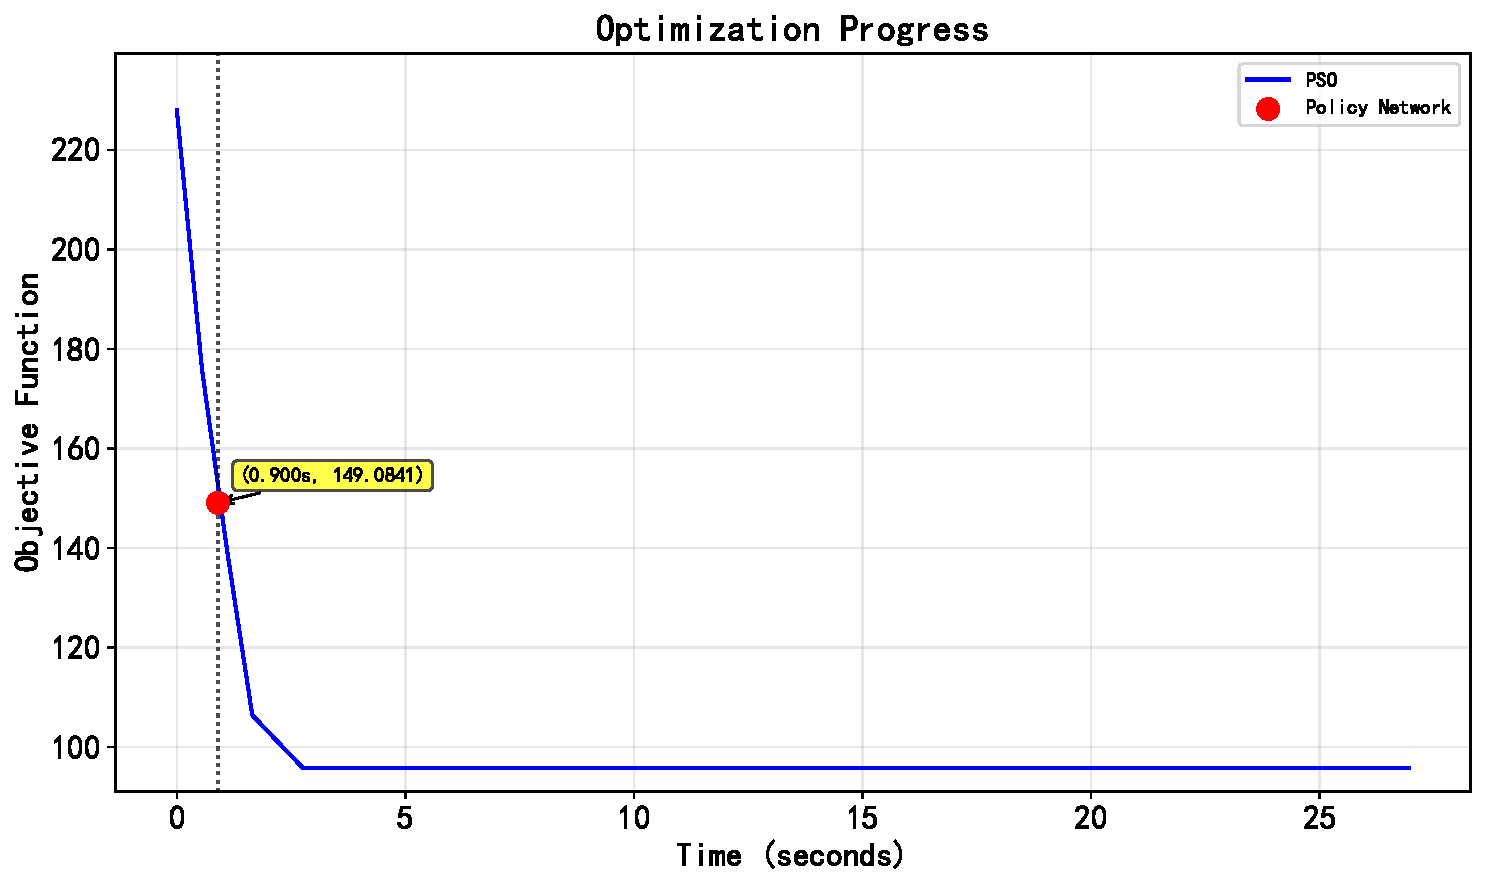
\includegraphics[width=9cm]{PSO-Objective_linear.pdf}}
\caption{Convergence curve of the objective function during PSO solving.}
\label{fig:pso_objective}
\end{figure}

In summary, PSO and the single-shot parametric decision are respectively insufficient in decision efficiency and safety, whereas the proposed method maintains an acceptable forging time and a decision speed far superior to PSO while guaranteeing no damage, and is thus more suitable for practical forging conditions.

  \section{Conclusion}

This paper proposes a forging world model and a continuous speed-profile decision method driven by it. The world model encodes the point cloud into a low-dimensional latent state with PointNet++, evolves this state continuously along the stroke with a Neural ODE that takes the speed profile as a physical prior, and jointly reconstructs the geometry and multi-physics fields with a DeepONet decoder (with the geometry using the first-step geometry as the residual baseline), realizing both the reconstruction and multi-step prediction of forging deformation. On this basis, the speed-profile decision is formulated as a finite-horizon Markov decision process with a damage constraint, and a continuous speed-profile policy is trained with offline safe reinforcement learning. Experiments show that the proposed method shortens the forging time while satisfying the damage constraint, with decision efficiency significantly superior to PSO, providing a feasible path toward intelligent decision-making of forging process parameters.

The validation of this work is still limited to the simulation data of a single press and a single forging (the 6082 aluminum alloy control arm), and both the world model and the policy are effective only within this scenario; moreover, the autoregressive error accumulates with the number of rollout steps. To build a general forging world model, it is necessary to collect large-scale simulation and measured data covering different forging shapes, material compositions, and process conditions, and to train larger models according to scaling laws. Its value lies not only in replacing finite element engines such as DEFORM with an AI surrogate model, but also in providing a cross-scenario propagatable environment for decision-making, so as to automatically generate speed profiles satisfying the damage constraint under different forgings and initial temperatures.

  \Acknowledgements{This work was supported by the National Science and Technology Major Project of the Ministry of Science and Technology of China (2024ZD0608100), the National Natural Science Foundation of China (62506031, 62332017, U22A2022), Fellowship from the China Postdoctoral Science Foundation (2026T190405), the Postdoctoral Fellowship Program of CPSF under Grant Number GZC20251093.}

\else
  \section{Introduction}
Forging is a core forming process in advanced equipment manufacturing.
As illustrated in Fig. \ref{fig:forging_press}, the workpiece undergoes
plastic deformation under compression between the upper and lower dies.
The forging speed, as a pivotal parameter, influences the
thermo-mechanical response and material dynamic softening behavior by
controlling the strain rate, thereby playing a decisive role in both
forming quality and efficiency.

However, this process is highly nonlinear, dynamically fast-changing,
and its internal state is often unmeasurable, making speed
decision-making a challenging open-loop control problem.
Traditional constant-speed strategies struggle to fully exploit material
dynamic softening, while variable-speed strategies present their own
difficulties: excessively high speeds can cause stress concentration and
damage, while excessively low speeds lead to increased deformation
resistance due to billet cooling, heightening the risk of cracking.
Consequently, rational planning of a speed profile to balance efficiency
and quality is of critical importance.

\begin{figure}[htbp]
\centerline{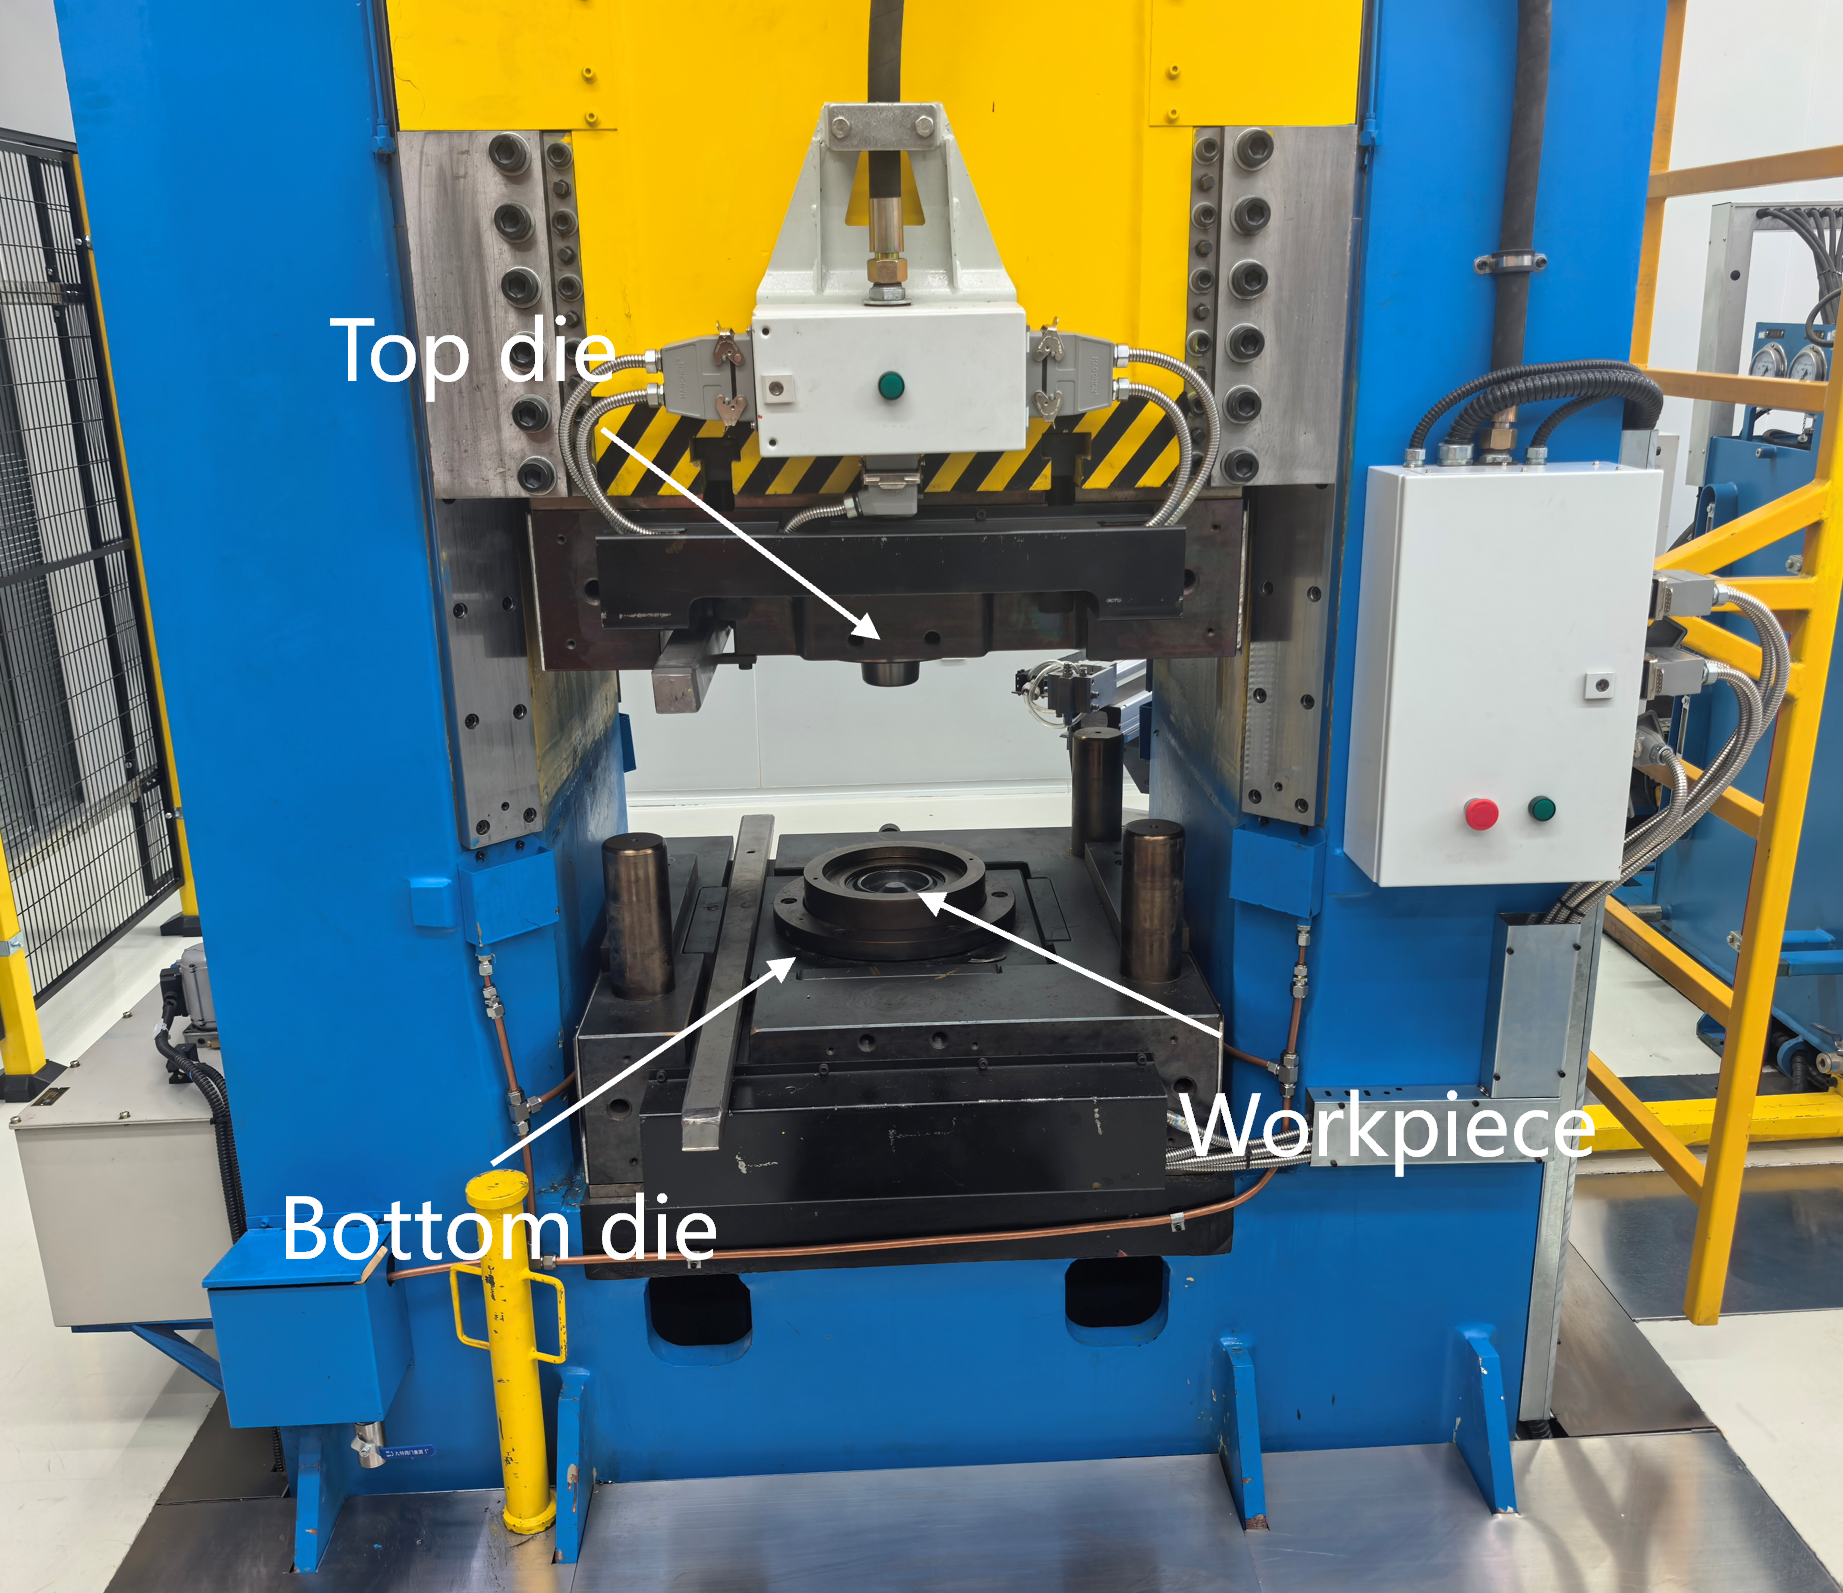
\includegraphics[width=\linewidth]{forging_press.png}}
\caption{Forging press.}
\label{fig:forging_press}
\end{figure}

% 为充分利用铝合金的动态软化特性\cite{lin2011critical}，本文提出"先慢后快"的变速策略：在变形初期以较低速度抑制应力集中，待材料进入软化阶段后逐步提高速度以兼顾效率。然而，实现该策略需解决高维非线性系统的优化控制难题。传统方法如模型预测控制(MPC)\cite{kouvaritakis2016model}优化速度慢，迭代学习控制(ILC)\cite{ahn2007iterative}依赖工况重复性，难以适应锻造过程的波动。
% 近年来，强化学习(RL)在机器人控制\cite{hafner2020mastering}等领域展现出强大潜力。例如，Stendal与Bambach\cite{stendal2024developing}提出了融合强化学习与有限元分析的协同仿真框架，用于钛铝合金塑性成形过程的智能控制，然而，该方法依赖于在线实时调整工艺参数的反馈机制，而真实锻造过程中显著的系统响应延迟使得此类闭环策略难以稳定实施；Dharmadhikari等人\cite{dharmadhikari2023reinforcement}则开发了基于无模型Q学习的强化学习框架，实现了增材制造工艺参数的自主优化。
% 这些方法均需在真实环境或仿真中进行在线学习。然而，真实锻造环境试验成本高、系统响应延迟长、设备操作风险大，完全不具备在线探索学习的条件，因此上述工作缺乏工程适用性。

% 离线强化学习(ORL)\cite{levine2020offline}通过基于历史数据学习策略，有效规避了在线交互的风险。DeepThermal\cite{zhan2022deepthermal}采用基于模型的ORL框架实现了发电机组的安全控制，Yuan等\cite{10705802}提出的时序批约束Q学习算法在浓密机控制中取得成效，验证了ORL在工业过程中的可行性。

% 然而，将离线强化学习应用于高维非线性锻造过程仍面临两大挑战：现有方法多依赖低维观测数据，难以准确表征锻造的多物理场耦合演化过程，亟需发展轻量化代理模型以替代昂贵的有限元仿真。此外，锻造设备的锻压速度属于高维连续动作，这导致策略学习与优化的复杂度显著提升。


% 针对上述挑战，本研究围绕铝合金锻造场景，重点研究：1.如何建立预测温度场、应力场与位移场全时域演化的高精度、高效率代理模型；2.如何基于离线强化学习，实现锻压速度曲线的低维参数化表征与开环优化，以生成满足多目标约束的高效设定曲线。主要贡献如下：




% 1．提出了基于深度算子网络的锻压过程代理模型架构，能够高精度、高效率地预测应力场、位移场等多物理场的时空演化过程，为策略学习提供了高效数据生成器。

% 2．提出了面向锻造场景多约束、多优化目标特点的离线安全强化学习范式。构建能够直接生成最优锻造速率曲线的优化控制器。
To fully exploit the dynamic softening characteristics of aluminum alloys
\cite{lin2011critical}, this paper proposes a "slow-then-fast"
variable-speed strategy. This approach employs a lower speed at the
initial deformation stage to mitigate stress concentration, and
subsequently increases the speed as the material enters the softening
stage to enhance efficiency. However, implementing this strategy
requires solving the optimal control problem of a high-dimensional
nonlinear system. Conventional methods, such as model predictive
control (MPC) \cite{kouvaritakis2016model}, suffer from slow
optimization speeds, while iterative learning control (ILC)
\cite{ahn2007iterative} relies on operating condition repeatability,
making them unsuitable for handling fluctuations in the forging process.

Recently, reinforcement learning (RL) has demonstrated considerable
potential in domains like robotic control \cite{hafner2020mastering}.
For instance, Stendal and Bambach \cite{stendal2024developing} developed
a co-simulation framework integrating RL with finite element analysis
for the intelligent control of Ti-Al alloy plastic forming. However,
their method depends on a feedback mechanism for online parameter
adjustment, which is challenging to implement stably in real forging due
to significant system response delays. Dharmadhikari et al.
\cite{dharmadhikari2023reinforcement} devised a model-free Q-learning
framework for autonomous optimization of additive manufacturing
parameters.

These methods, however, require online learning in either real or
simulated environments. Conducting online exploration in real forging is
impractical due to high costs, long delays, and operational risks, thus
limiting the engineering applicability of the aforementioned approaches.

Offline reinforcement learning (ORL) \cite{levine2020offline} overcomes
this limitation by learning policies directly from historical datasets,
effectively avoiding the risks of online interaction. For example,
DeepThermal \cite{zhan2022deepthermal} employed a model-based ORL
framework for safe control of power units, and Yuan et al.
\cite{10705802} achieved effective control in thickener operation with a
temporal batch-constrained Q-learning algorithm, validating ORL's
feasibility in industrial processes.

Nevertheless, applying ORL to high-dimensional nonlinear forging poses
two major challenges. First, existing methods often rely on
low-dimensional observational data, which is insufficient to characterize
the coupled multi-physics evolution, necessitating a lightweight
surrogate model to replace costly finite element simulations. Second,
the forging speed constitutes a high-dimensional continuous action,
significantly increasing the complexity of policy learning and
optimization.

To address these challenges, this study focuses on aluminum alloy
forging and investigates: 1) establishing a high-precision and efficient
surrogate model for predicting the full-time evolution of temperature,
stress, and displacement fields; and 2) leveraging ORL to achieve
low-dimensional parameterization and open-loop optimization of the speed
profile, generating an efficient set-point curve that satisfies multiple
constraints. The main contributions are as follows:

1. We propose a surrogate model architecture for the forging process
based on the deep operator network, which enables highly accurate and
efficient prediction of the spatiotemporal evolution of multi-physics
fields (e.g., stress and displacement), serving as an efficient data
generator for policy learning.

2. We propose an offline safe RL paradigm tailored for the
multi-constraint, multi-objective nature of forging. An optimal control
agent is developed to directly generate the optimal forging speed curve.

The overall framework of this research is illustrated in
Fig. \ref{fig:framework}. It consists of two stages: a point-cloud world
model is first learned from simulation data to act as a fast and
differentiable environment, and a model-based policy is then trained
within this environment to generate the forging speed curve.

\begin{figure}[htbp]
\centerline{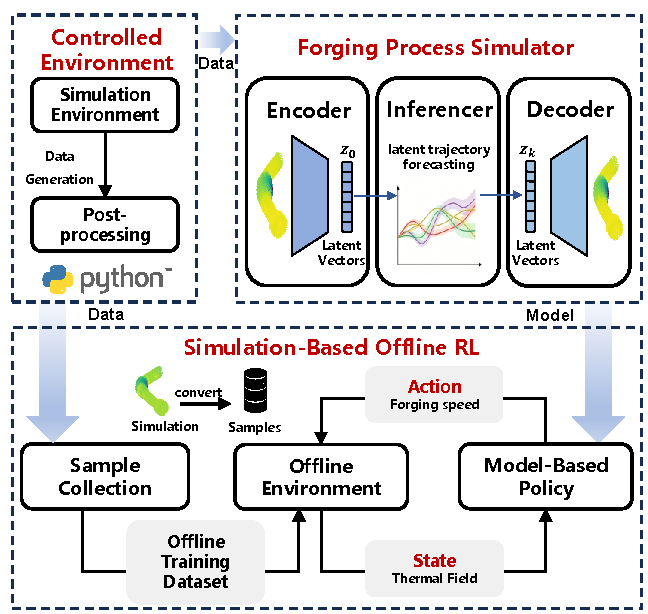
\includegraphics[width=\linewidth]{frame-1.pdf}}
\caption{The framework of this research.}
\label{fig:framework}
\end{figure}

  \section{Preliminaries}

\subsection{点云表征}
点云以一组三维点表示工件表面，每个点除坐标外还可携带温度、应力等物理量，记为 $X=\{x_i\}_{i=1}^{N}$，$x_i\in\mathbb{R}^{C}$。点云是无序集合，同一形状对应 $N!$ 种排列，故处理点云的模型需具备置换不变性~\cite{qi2017pointnet}。与规则网格相比，点云不受拓扑与分辨率限制，可直接表示任意几何形状，适合承载有限元仿真输出的几何与场量。

\subsection{连续时间隐状态建模}
Neural ODE 以参数化的向量场描述状态的连续演化：给定初值 $c(s_0)=c_0$，任意位置的状态由
\begin{equation}
\frac{\mathrm{d}c}{\mathrm{d}s}=g(c,s;\theta)
\end{equation}
积分得到~\cite{chen2018neural}。与离散时间递推相比，它以连续自变量刻画动力学，可在任意时刻求值，并可用伴随法反向传播。这类模型已在工业过程的连续时间建模中得到应用~\cite{yuan2022autonomous, yuan2023ode, yuan2022differential}。

\subsection{世界模型}
世界模型将高维观测压缩为低维隐状态，并在隐空间中学习状态随动作的演化，从而在不与真实环境交互的条件下预测未来。典型结构含编码器、推理器与解码器三部分：编码器由观测得到隐状态，推理器预测下一时刻的隐状态，解码器将隐状态还原为观测。预测在低维空间完成，计算代价远低于直接在高维观测上推演。

\subsection{DeepONet}
DeepONet 用于学习函数到函数的映射，由 branch 与 trunk 两个子网构成：branch 接收输入函数的离散采样，trunk 接收输出函数的自变量，二者输出做内积即得该自变量处的函数值~\cite{lu2021deeponet}。由于输出是自变量的连续函数，模型可在任意位置给出预测，无需预先固定离散网格。

  \section{Problem Formulation}

\subsection{锻造变形序列与状态表征}
铝合金锻造过程中，工件在上、下模具间受压发生塑性变形，其几何形状与温度、等效应力、损伤等物理量随变形历程同步且连续地演化。锻造历程中第 $k$ 步的工件状态以无序点云 $X_k \in \mathbb{R}^{N \times 6}$ 表示，其中 $N$ 为采样点数，每个点由绝对坐标 $p_i=(x_i,y_i,z_i)$ 与温度 $T_i$、等效（von Mises）应力 $\sigma_i$、损伤 $D_i$ 三个物理场组成：
\begin{equation}
X_k = \{\,(p_i,\; T_i,\; \sigma_i,\; D_i)\,\}_{i=1}^{N}
\label{equ:pointcloud}
\end{equation}
其中等效应力由六个应力分量按物理量纲合成：
\begin{equation}
\begin{split}
\sigma = \Big\{ &\tfrac{1}{2}\big[(\sigma_x-\sigma_y)^2+(\sigma_y-\sigma_z)^2 \\
&+(\sigma_z-\sigma_x)^2\big]+3(\tau_{xy}^2+\tau_{yz}^2+\tau_{xz}^2)\Big\}^{1/2}
\end{split}
\end{equation}
温度随热传导与变形生热连续渐变；等效应力与损伤由当前几何与整个变形历程共同决定，具有路径相关性。因此，锻造状态是高维、无序、且几何与多物理场强耦合的点云序列，其演化在时间上连续。

\subsection{控制变量与物理约束}
本文的控制决策变量是整个锻造时间域 $[0,t_f]$（即 $[0,T]$，其中 $T=t_f$ 为锻造总时长）上的完整下压速度函数 $v_y(\cdot)=\{v_y(t)\mid t\in[0,t_f]\}$。该曲线在下压开始前确定，并在锻造过程中开环执行。下压速度通过改变应变速率影响应力场与损伤演化：速度过高引发应变率强化与应力集中，速度过低则延长锻造时间、加剧工件温降与变形抗力。

锻造过程中压机行程 $\Delta h$ 恒定，要求速度曲线在整个锻造时长 $t_f$ 上的积分固定：
\begin{equation}
\int_{0}^{t_f} v_y(t)\,dt = \Delta h = \text{const}
\end{equation}
锻造质量由损伤判据约束。基于 Normalized Cockcroft--Latham 准则，
\begin{equation}
D(t) = \int_0^t \frac{\max(\sigma_1(\tau),0)}{\bar{\sigma}(\tau)}\,\dot{\bar{\varepsilon}}(\tau)\,d\tau
\end{equation}
记临界损伤值为 $D_{\text{cr}}$，损伤累积值一旦超过它即视为开裂。锻造要求全程损伤不超该临界值，即 $D(t) < D_{\text{cr}},\ \forall t\in[0,t_f]$。

在上述物理过程与约束下，本文要解决的问题可分解为如下两个相互关联的子问题。

\textbf{问题一（连续演化建模）}：给定初始步点云 $X_0$ 与下压速度曲线 $v_y(t)$，如何预测工件几何与温度、等效应力、损伤等多物理场在变形历程中的连续演化，并获得紧凑、可推演的状态表征，使模型既能由此预测未来各步的状态，又能高保真地还原为几何—多物理场点云？
    
\textbf{问题二（连续速度曲线决策）}：在恒定锻造行程与损伤约束下，如何决策整条连续速度曲线 $v_y(t)$，使锻造时间 $t_f$ 最短，同时保证损伤全程不超过临界值 $D_{\text{cr}}$？

综合两个子问题，最终要求解的下压速度决策问题可写成如下约束优化形式：
\begin{equation}
\begin{gathered}
\min\nolimits_{v_y(t)} \; t_f \\
\text{s.t.} \quad \int_{0}^{t_f} v_y(t)\,dt = \Delta h \\
D(t) < D_{\text{cr}}, \quad \forall t \in [0, t_f]
\end{gathered}
\label{equ:model}
\end{equation}
即在恒定锻造行程前提下，兼顾生产效率与成形质量，寻求最优速度曲线。

  \section{Forging Process Simulator}
% 本研究构建了一个基于深度算子网络（DeepONet）的代理模型，用于在给定锻压参数下同步预测位移场、应力场和损伤场的时空演化。该模型学习由控制量与扰动决定的物理场预测算子，实现多场耦合与全时域一体化建模。

% 锻造过程被表述为依赖于初始温度场和工艺参数的演化问题。模型输入包括工艺参数（分支网络处理的速度曲线参数 $\theta = \{v_0, v_1, t_0, t_1\}）$和时空信息（主干网络处理的空间坐标$ (x, y, z)、SDF、时间步step 和初始温度 Temp）$。基于算子学习框架，模型具备全时域预测能力，一次前向传播即可直接输出对应时间步 step 的物理状态，结构如图\ref{fig:model}所示。
% \begin{figure}[htbp]
% \centerline{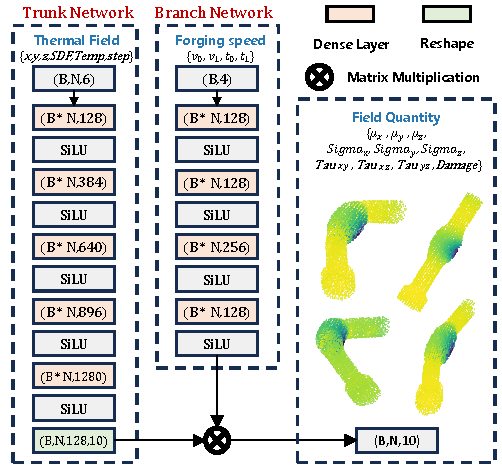
\includegraphics[width=\linewidth]{model.pdf}}
% \caption{Field value prediction model.}
% \label{fig:model}
% \end{figure}

% 模型目标是学习一个算子G，建立如下映射关系：
% \begin{equation}
% G:(\theta)(x,y,z,SDF,step,Temp)\to(\mu,\sigma,d)
% \end{equation}
% 其中 $\mu$、$\sigma$ 和 $d$ 分别表示位移场、应力场和损伤场。为捕捉变形与应力的强耦合关系，模型采用共享输出层设计：分支网络提取参数特征 $B = [b_1, b_2, \dots, b_p]$，主干网络提取时空特征$ T = [t_1, t_2, \dots, t_q]$，二者融合后通过共享权重输出联合物理场：
% % \begin{equation}
% %     \mathbf{y}(x,y,z,step) \approx W \cdot (B \otimes T) + b_0
% % \end{equation}

% % \begin{equation}
% % \begin {split}
% %  \mathbf{y}(x,y,z, step) &= [u(x,y,z, step), \\
% %      &\sigma(x,y,z, step), d(x,y,z,step)]
% % \end{split}
% % \end{equation}

% \begin{equation}
% \begin{split}
% \mathbf{y}(x,y,z,step) &\approx W \cdot (B \otimes T) + b_0 \\
% \mathbf{y}(x,y,z, step) &= [u(x,y,z, step), \\
%      &\sigma(x,y,z, step), d(x,y,z,step)]
% \end{split}
% \end{equation}

% 其中$W$是共享输出层的权重矩阵，$b_0$是偏置向量。该设计通过统一映射机制同步输出多物理场，强化了耦合关系学习，保障了物理一致性。

% 训练过程通过最小化预测与真实数据之间的均方误差进行：
% \begin{equation}
% \mathcal{L} = \frac{1}{N} \sum_{i=1}^{N}
% \left\|
% \left[ \mathbf{y}^{(i)} \right] -
% \left[ \mathbf{y}_\text{true}^{(i)} \right]
% \right\|^2
% \end{equation}
This work develops a DeepONet-based surrogate model to predict the
coupled spatiotemporal evolution of displacement, stress, and damage
fields during forging. The model learns the underlying physics operator
for full-time-domain prediction.

The process is modeled as an evolution problem dependent on the initial
temperature field and speed parameters
$\theta = \{v_0, v_1, t_0, t_1\}$. Inputs are $\theta$ (branch net) and
spatiotemporal coordinates $(x, y, z, SDF, step, Temp)$ (trunk net). A
single forward pass outputs the state at any given time step
(Fig. \ref{fig:model}).

The model learns the operator $G$:
\begin{equation}
G: (\theta)(x, y, z, SDF, step, Temp) \rightarrow (u, \sigma, d)
\end{equation}
where $u$, $\sigma$, $d$ are displacement, stress, and damage. A shared
output layer captures field couplings. Branch and trunk outputs $B$ and
$T$ are fused as:
\begin{equation}
\mathbf{y} = [u, \sigma, d] = W \cdot (B \otimes T) + b_0
\end{equation}
This unified mapping ensures physical consistency. Training minimizes
the mean squared error:
\begin{equation}
\mathcal{L} = \frac{1}{N} \sum_{i=1}^{N} \left\| \mathbf{y}^{(i)} - \mathbf{y}_{\text{true}}^{(i)} \right\|^2
\end{equation}

  \section{Forging Optimization Control}
% 本节提出一种基于安全离线强化学习的锻造优化控制训练框架，通过离线训练使智能体根据锻件初始温度场，在满足损伤约束的前提下，直接生成完整锻造过程的最优速度曲线，实现开环规划，具体如图\ref{fig:control-1}所示。

% 为求解该问题，将过程建模为上下文赌博机模型\cite{bouneffouf2020survey}，其元组 $(\mathcal{S}, \mathcal{A}, \mathcal{R}, \mathcal{C})$ 定义如下：

% \textbf{状态空间$\mathcal{S}$}：观测状态$\mathbf S\in\mathcal{S}$为锻件中$N$个微元的位置和温度,其中每个微元表示为$\mathbf{s}_i=\{x_i, y_i, z_i, T_i\}$，完整观测状态$\mathbf{S}\in\mathbb{R}^{N*4}$。

% \textbf{动作空间$\mathcal{A}$}：锻造速度决策$\mathbf a\in \mathcal{A}$采用四个参数$\mathbf a =[v_0,v_1,t_0,t_1]$进行表示，其与曲线的映射关系见章节\ref{sec:speed}。

% \textbf{奖励$R$}：定义为锻造效率与锻件内部应力的加权组合
% \begin{equation}
%   R = \underbrace{w_1 \cdot \exp(-time)}_{\text{time\_reward}} - \underbrace{w_2  \cdot \exp(stress)}_{\text{stress\_penalty}}
% \end{equation}
% 作为奖励,其中$\text{stress\_penalty}$奖励较小应力，$\text{time\_reward}$奖励生产效率，$w_i$为权重系数。

% \textbf{安全约束$\mathcal{C}$}：基于Normalized Cockcroft \& Latham断裂准则计算损伤值:
% \begin{equation}
% D(t) = \int_{0}^{t} \frac{\max(\sigma_1(\tau), 0)}{\bar{\sigma}(\tau)} \dot{\bar{\varepsilon}}(\tau) d\tau
% \end{equation}
% 损伤累积值$D(t)$来表征$C$，它是材料在变形过程中，其最大拉应力与等效应力之比乘上当前应变随时间的积分值，
% 当$C$超过材料临界损伤$C_0$时视为断裂。

% 本研究的目标是从有限元仿真生成的静态数据集 $\mathcal{B} = \{ (s_i, a_i, r_i, c_i) \}_{i=1}^{N}$中学习最优策略网络 $\pi^{*}$,在满足成本约束的前提下最大化奖励。所有策略的训练与评估均基于数据集 $\mathcal{B}$离线完成，无需与实际锻压设备交互。
This section proposes a safe offline reinforcement learning framework
for forging optimization. The agent is trained offline to generate an
optimal speed profile based on the initial temperature field, satisfying
damage constraints for open-loop planning (Fig. \ref{fig:control-1}).

The problem is formulated as a contextual bandit model
\cite{bouneffouf2020survey}, defined by the tuple
$(\mathcal{S}, \mathcal{A}, \mathcal{R}, \mathcal{C})$:

\textbf{State space $\mathcal{S}$}: The observation state
$\mathbf{S} \in \mathcal{S}$ comprises the positions and temperatures of
$N$ micro-elements in the workpiece,
$\mathbf{s}_i = \{x_i, y_i, z_i, T_i\}$, forming
$\mathbf{S} \in \mathbb{R}^{N \times 4}$.

\textbf{Action space $\mathcal{A}$}: The forging speed decision
$\mathbf{a} \in \mathcal{A}$ is parameterized as
$\mathbf{a} = [v_0, v_1, t_0, t_1]$, mapping to a curve as defined in
Section \ref{sec:speed}.

\textbf{Reward $\mathcal{R}$}: A weighted combination of efficiency and
internal stress:
\begin{equation}
R = \underbrace{w_1 \cdot \exp(-\text{time})}_{\text{time\_reward}} - \underbrace{w_2 \cdot \exp(\text{stress})}_{\text{stress\_penalty}}
\end{equation}
where the time reward promotes productivity and the stress penalty
discourages high stress.

\textbf{Cost $\mathcal{C}$}: Damage is evaluated via the normalized
Cockcroft \& Latham criterion:
\begin{equation}
D(t) = \int_{0}^{t} \frac{\max(\sigma_1(\tau), 0)}{\bar{\sigma}(\tau)} \dot{\bar{\varepsilon}}(\tau) d\tau
\end{equation}
Cost $C$ is the cumulative damage $D(t)$. Fracture occurs when $C$
exceeds the critical value $C_0$.

The objective is to learn an optimal policy $\pi^*$ from a static
dataset $\mathcal{B} = \{ (s_i, a_i, r_i, c_i) \}_{i=1}^{N}$ generated
by finite element simulations, maximizing reward while satisfying the
cost constraint. All policy training and evaluation is performed offline
on $\mathcal{B}$, with no interaction with the physical forging
equipment.

\begin{figure}[htbp]
\centerline{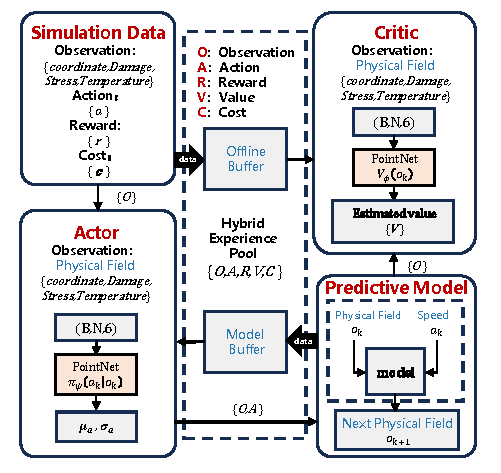
\includegraphics[width=\linewidth]{control-1.pdf}}
\caption{Training architecture of policy network .}
\label{fig:control-1}
\end{figure}
% 决策网络基于 PointNet\cite{qi2017pointnet} 架构构建，实现了温度场到速度曲线参数的映射。
% 决策网络训练使用混合经验池，包含当前策略生成的交互数据与历史仿真数据。为实现带约束的策略优化，可引入拉格朗日松弛法将原约束问题转化为无约束形式。具体地，构造拉格朗日函数：
% \begin{equation}
% L(\psi, \lambda) = \mathbb{E}_{ p_{\psi}} \left[ \ln p_{\psi}(a|
% s) \cdot A(s,a) \right]
% \end{equation}
% 其中,优势函数为：
% \begin{equation}
% A(s,a) = R - V(s) - \lambda \cdot \mathrm{relu}(c - c_0)
% \end{equation}
% V(s)是通过蒙特卡洛采样估计的期望奖励。对于给定的初始状态$s$，从当前策略网络 $\pi_{\psi}(a|s)$中蒙特卡洛采样 $N$个动作 $\{a_{j} \}_{j=1}^N$，每个动作 $a_j$对应一条速度曲线。将这些动作输入代理模型，预测场量状态，计算每个动作的奖励 $R(a_j)$，然后取平均值作为价值估计：
% \begin{equation}
% V(s) = \mathbb{E}_{a \sim \pi_{\psi}(\cdot|s)} [R(s, a)] \approx \frac{1}{N} \sum_{j=1}^{N} R(s, a_j)
% \end{equation}

% 为鼓励策略探索并防止过早收敛，在优化目标中加入熵正则化项：
% \begin{equation}
% J(\psi, \lambda) = L(\psi, \lambda) + \eta H[a|s)]
% \end{equation}
% 该优化问题通过对偶梯度上升法求解：在每一步迭代中，首先固定对偶变量 $\lambda$，通过梯度上升更新策略参数 $\psi$ 以最大化拉格朗日函数；然后固定策略参数 $\psi$，根据约束违反程度更新对偶变量 $\lambda$。对偶变量的更新规则为：
% \begin{equation}
% \lambda \leftarrow \max(0, \lambda + \alpha_{\lambda} (c - c_0))
% \end{equation}
% 当损伤值 $c$ 超过阈值 $c_0$ 时，对偶变量 $\lambda$ 增加以加强约束惩罚，反之则减小惩罚力度。

The policy network, built on the PointNet architecture
\cite{qi2017pointnet}, maps the temperature field to speed profile
parameters. It is trained using a hybrid experience replay buffer
containing data from both the current policy and historical simulations.

Constrained policy optimization is achieved via Lagrangian relaxation,
transforming the problem into an unconstrained form. The Lagrangian is
defined as:
\begin{equation}
L(\psi, \lambda) = \mathbb{E}_{p_{\psi}} \left[ \ln p_{\psi}(a|s) \cdot A(s,a) \right]
\end{equation}
with the advantage function:
\begin{equation}
A(s,a) = R - V(s) - \lambda \cdot \mathrm{relu}(c - c_0)
\end{equation}
Here, $V(s)$ is the expected reward estimated via Monte Carlo sampling.
Given an initial state $s$, $N$ actions $\{a_j\}_{j=1}^N$ are sampled
from the current policy $\pi_{\psi}(a|s)$. Each action $a_j$ corresponds
to a speed profile. The surrogate model predicts the resulting field
states, and the value is estimated as:
\begin{equation}
V(s) \approx \frac{1}{N} \sum_{j=1}^{N} R(s, a_j)
\end{equation}

To encourage exploration and prevent premature convergence, an entropy
regularization term is added:
\begin{equation}
J(\psi, \lambda) = L(\psi, \lambda) + \eta H[a|s]
\end{equation}
The optimization is solved using dual gradient ascent. In each
iteration, the policy parameters $\psi$ are updated to maximize $J$ with
fixed $\lambda$, and then the dual variable is updated based on
constraint violation:
\begin{equation}
\lambda \leftarrow \max(0, \lambda + \alpha_{\lambda} (c - c_0))
\end{equation}
This increases the penalty when the damage $c$ exceeds the threshold
$c_0$, and decreases it otherwise.

  \section{Experiment}
\subsection{Dataset and Settings}


% 本研究基于Deform-3D构建了600组锻造仿真数据集，重点控制初始温度场与锻造速度。通过模拟冷却过程获得10组非均匀初始温度场；通过参数$\theta=\{v_0,v_1,t_0,t_1\}$生成60组速度曲线$v_y(t)$。每个案例输出温度、应力、变形、损伤等多物理场数据，以点云形式存储，每时间步约5000个点，记录坐标$(x, y, z)$及各物理量。

This study established a dataset of 600 forging simulations using
Deform-3D, with controlled variations in the initial temperature field
and forging speed. Ten non-uniform initial temperature fields were
generated by simulating the cooling process. Sixty distinct speed
profiles $v_y(t)$ were produced by varying the parameters
$\theta = \{v_0, v_1, t_0, t_1\}$. Each simulation outputs multi-physics
field data (temperature, stress, strain, damage), stored as point clouds
containing approximately 5,000 points per time step. Each point records
its coordinates $(x, y, z)$ and the corresponding physical quantities.

\subsection{Evaluation of the Simulator}
% 为评估模型对物理场的预测精度，以应力场为例，将模型预测点云与有限元仿真结果对比。如图\ref{fig:model_result}所示，不同工况下预测与真实应力分布高度一致，表明模型能准确捕捉场量的空间分布特征。误差分析显示，偏差集中于局部区域且幅度较小。训练与测试阶段的均方误差分别为0.1780和0.2200，表明模型在场量预测中具有较好精度，能有效学习不同工况下的物理场分布规律。

The predictive accuracy of the surrogate model is evaluated by comparing
its stress field predictions against finite element simulation results.
As shown in Fig. \ref{fig:model_result}, the predicted and actual stress
distributions exhibit strong agreement under various working conditions,
demonstrating the model's capability to accurately capture spatial field
characteristics. Error analysis indicates that deviations are localized
and minimal. With mean squared errors of 0.1780 (training) and 0.2200
(testing), the model demonstrates high precision in field prediction and
effectively learns the distribution patterns of physical fields across
different conditions.

\begin{figure}[htbp]
\centerline{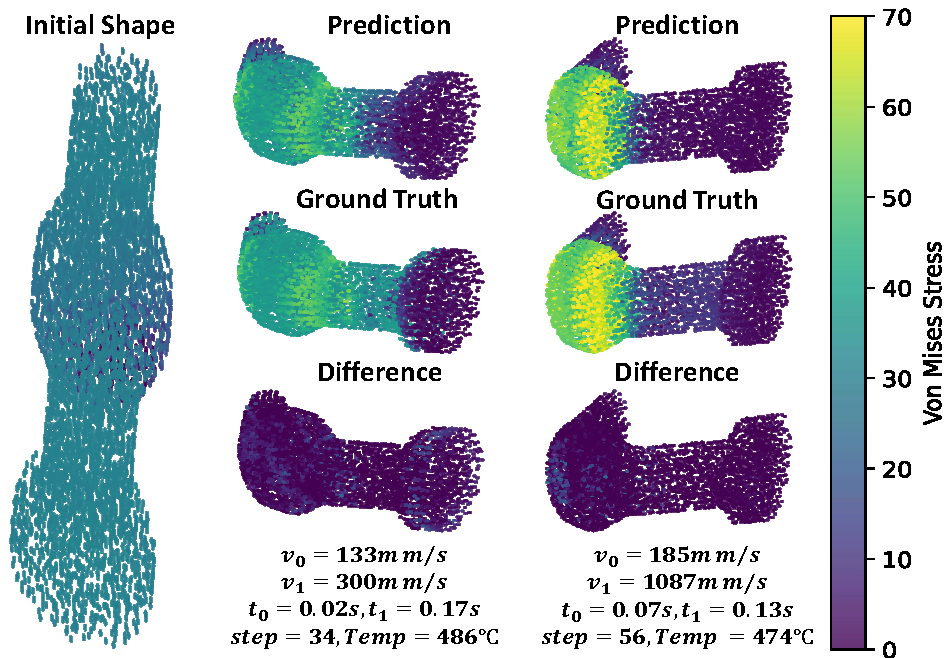
\includegraphics[width=\linewidth]{model_result-1.pdf}}
\caption{Comparison of model predictions and FEA results.}
\label{fig:model_result}
\end{figure}




\subsection{Evaluation on Offline RL}
% 强化学习结果如图\ref{fig:reward_a}与\ref{fig:damage_b}所示。平均奖励从波动上升至稳定正值（图\ref{fig:reward_a}），表明策略收敛；损伤值后期稳定低于$c_0=0.43$（图\ref{fig:damage_b}），满足安全约束。结果表明，该方法兼具优化能力与约束满足性，适用于锻造工艺决策。

The reinforcement learning results are shown in Figs. \ref{fig:reward_a}
and \ref{fig:damage_b}. The average reward rises from fluctuations to a
stable positive value (Fig. \ref{fig:reward_a}), indicating policy
convergence, while the damage value stabilizes below the threshold
$c_0 = 0.43$ (Fig. \ref{fig:damage_b}), confirming constraint
satisfaction. These results demonstrate that the proposed method
effectively balances optimization performance with safety compliance,
validating its applicability to forging process decision-making.



% \begin{figure}[htbp]
% \centerline{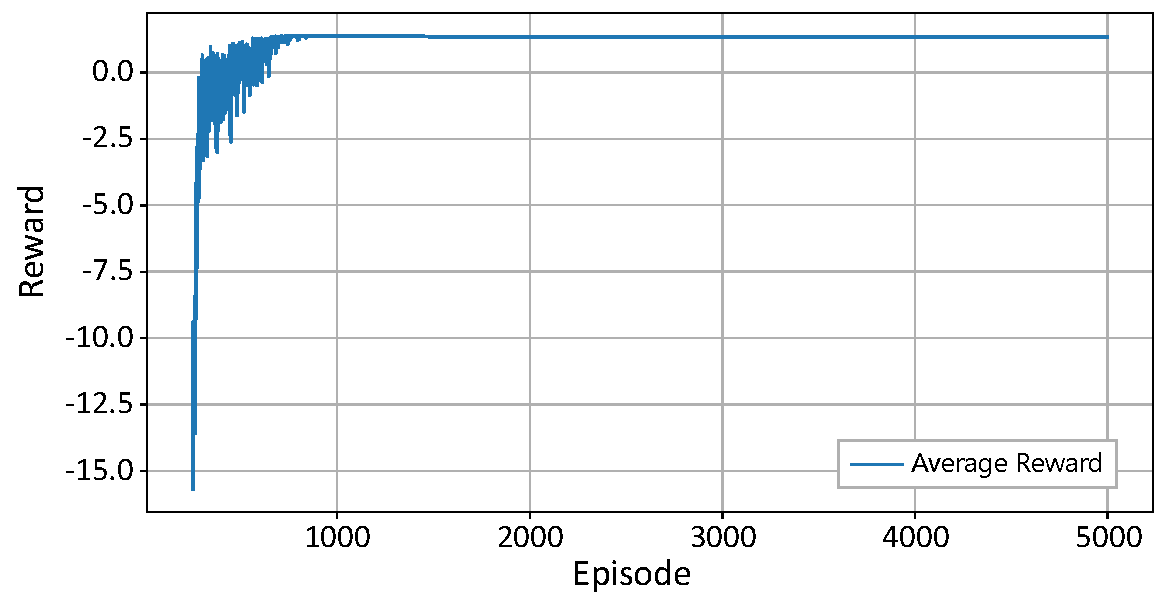
\includegraphics[width=\linewidth]{reward-1.pdf}}
% \caption{Training reward over epochs.}
% \label{fig:reward_a}
% \end{figure}


% \begin{figure}[htbp]
% \centerline{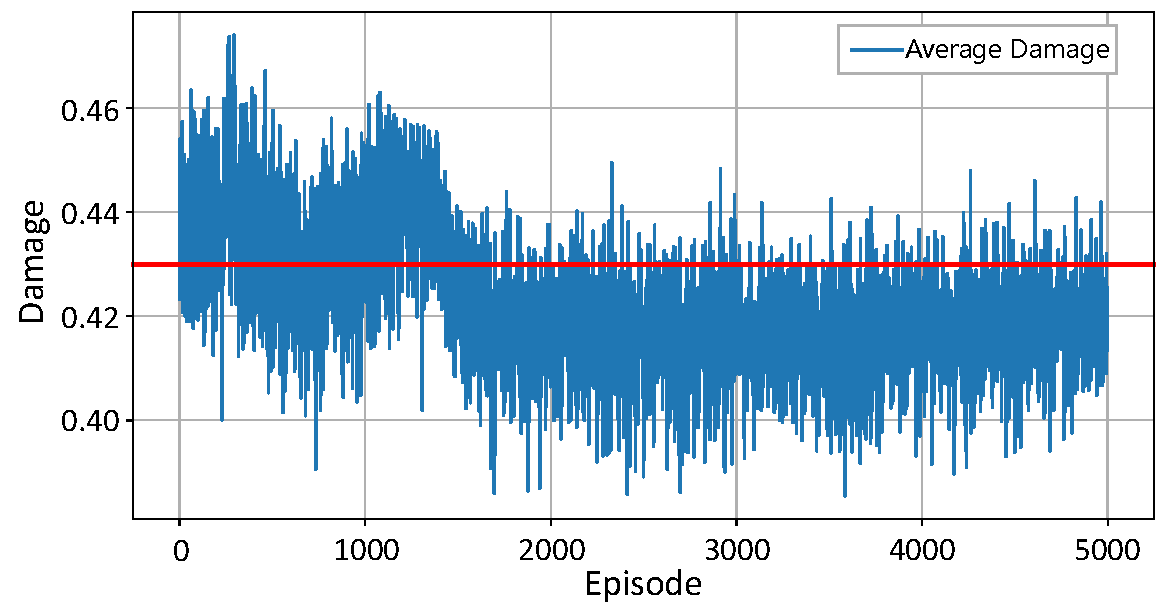
\includegraphics[width=\linewidth]{damage-1.pdf}}
% \caption{Training damage over epochs.}
% \label{fig:damage_b}
% \end{figure}

\begin{figure}[htbp]
    \centering
    \begin{subfigure}{0.48\columnwidth}
        \centering
        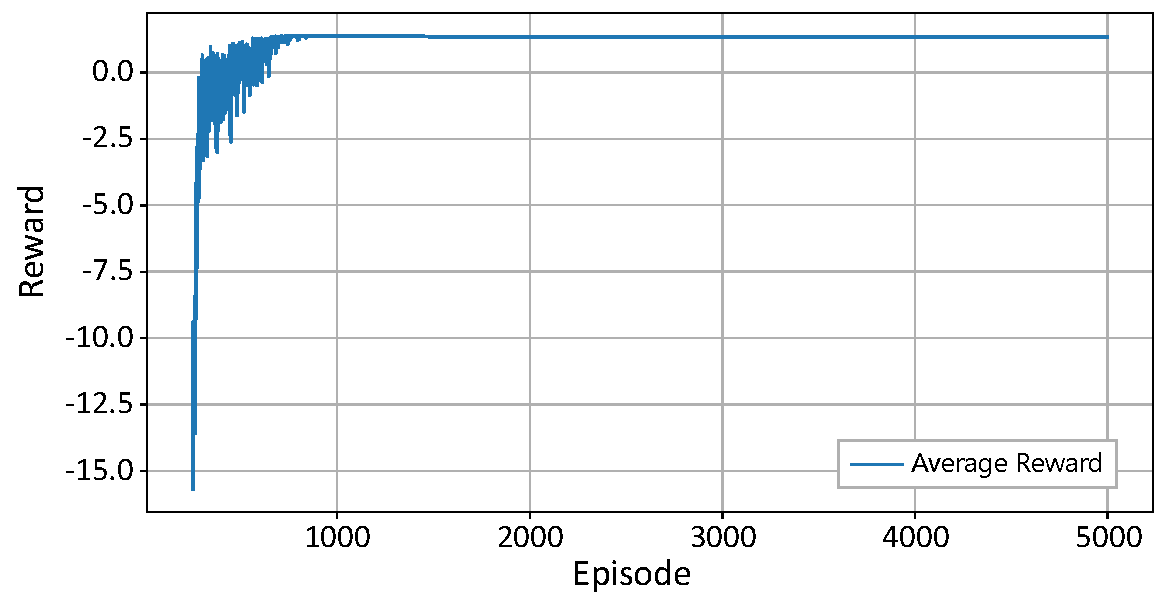
\includegraphics[width=\linewidth]{reward-1.pdf}
        \caption{Reward}
        \label{fig:reward_a}
    \end{subfigure}
    \hfill
    \begin{subfigure}{0.48\columnwidth}
        \centering
        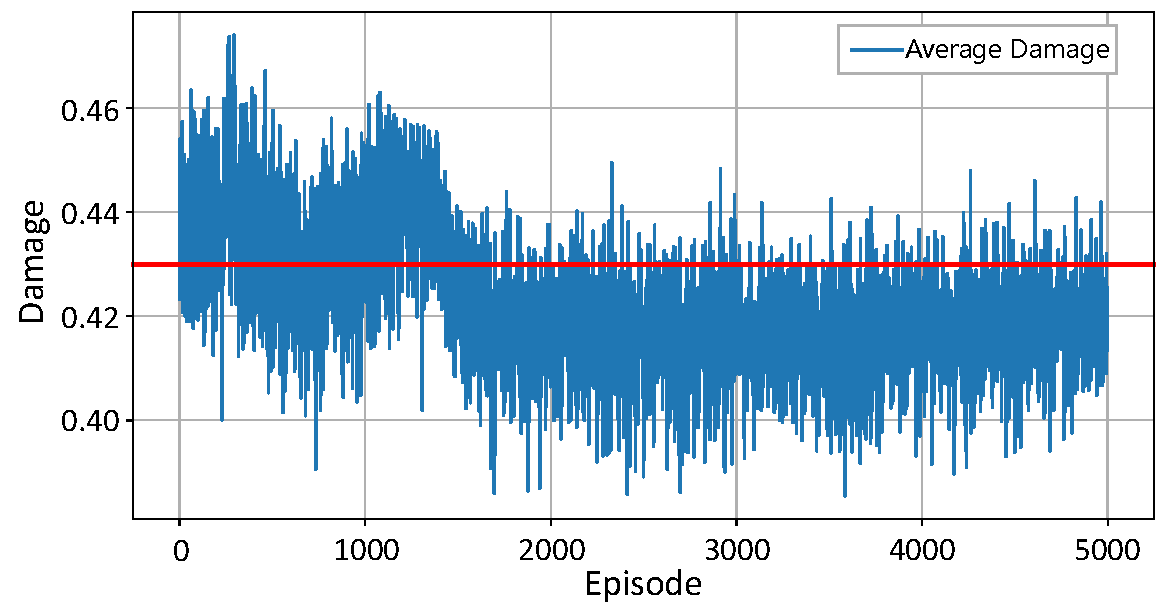
\includegraphics[width=\linewidth]{damage-1.pdf}
        \caption{Damage}
        \label{fig:damage_b}
    \end{subfigure}
    \caption{Training parameter over epochs.}
    \label{fig:combined_curves}
\end{figure}


% \begin{figure}[htbp]
% \centerline{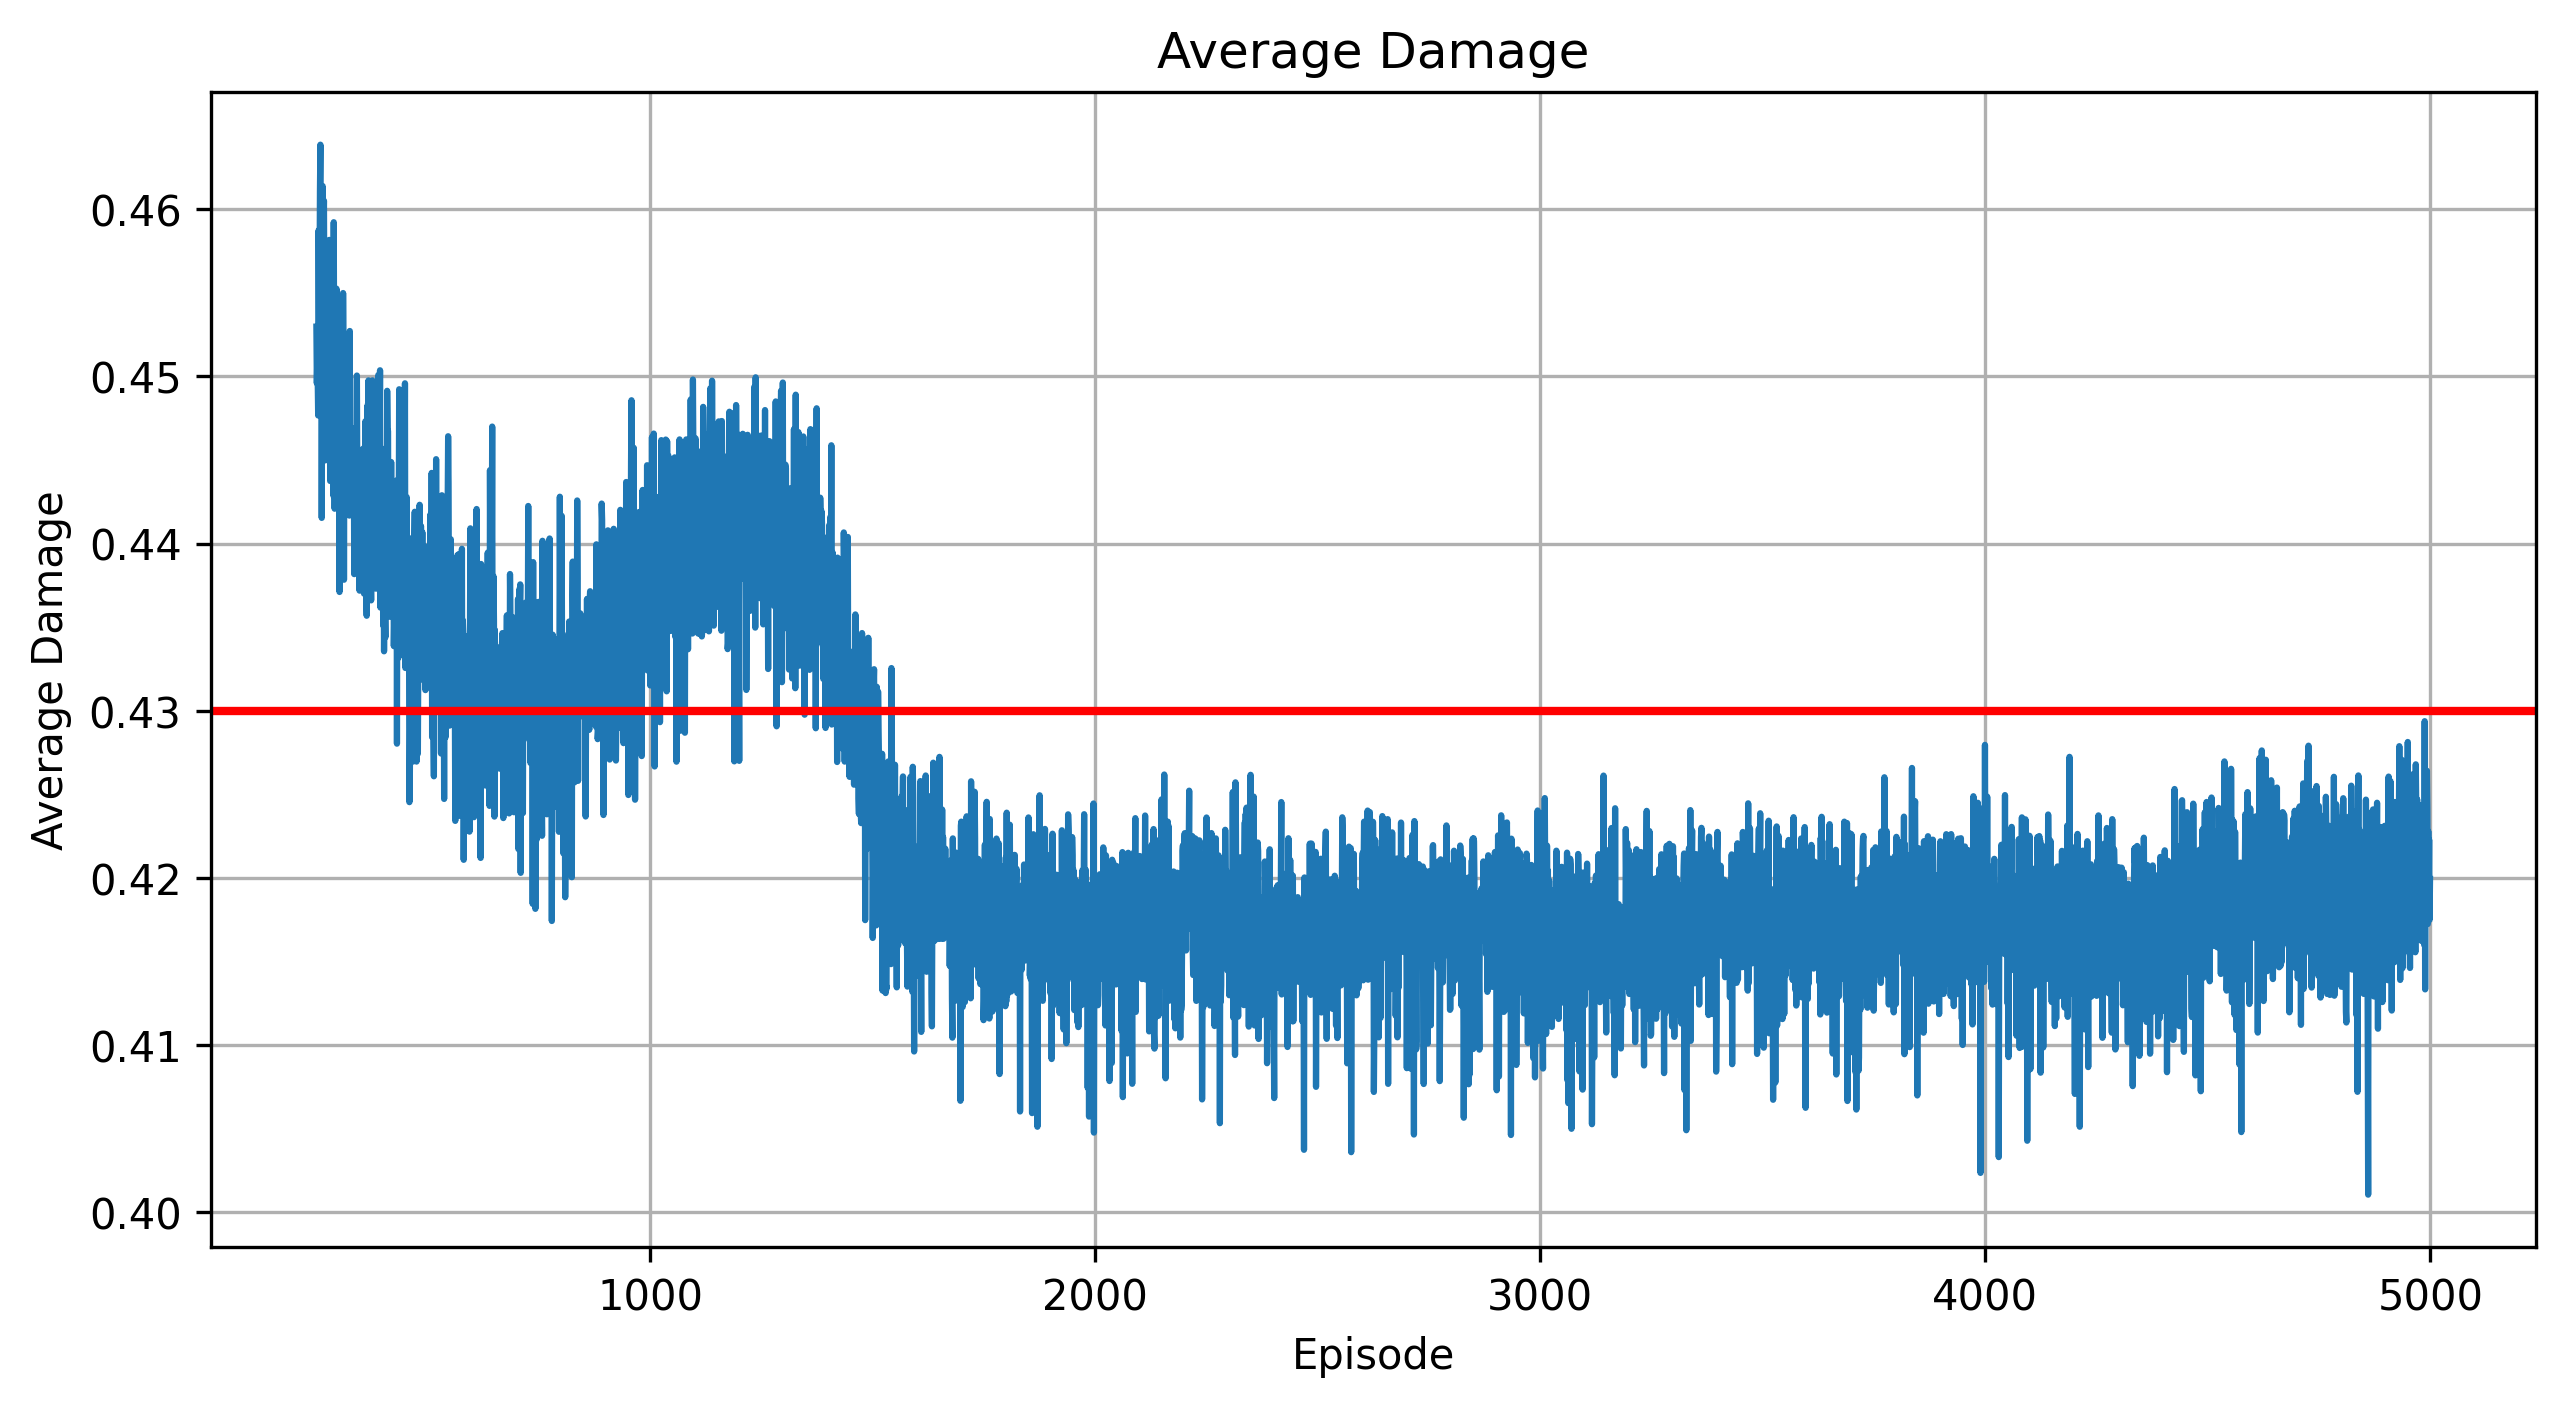
\includegraphics[width=\linewidth]{damages_episode_4999.png}}
% \caption{Example of a figure caption.}
% \label{fig:damages_episode_4999}
% \end{figure}

% 图\ref{fig:NetworkSpeed_a}展示了不同温度场下的速度曲线。当温度从$474^{\circ}C$升至$500^{\circ}C$时，速度曲线加速段提前，锻造时间缩短，表明决策网络能根据温度自适应调整策略，以应对材料高温软化特性。

Fig. \ref{fig:NetworkSpeed_a} presents the speed profiles under
different temperature fields. As the temperature increases from
$474\,^{\circ}\mathrm{C}$ to $500\,^{\circ}\mathrm{C}$, the acceleration
phase of the speed curve occurs earlier, reducing the total forging
time. This demonstrates the policy network's ability to adaptively
adjust the strategy based on temperature, effectively responding to the
material's high-temperature softening characteristics.

% \begin{figure}[htbp]
% \centerline{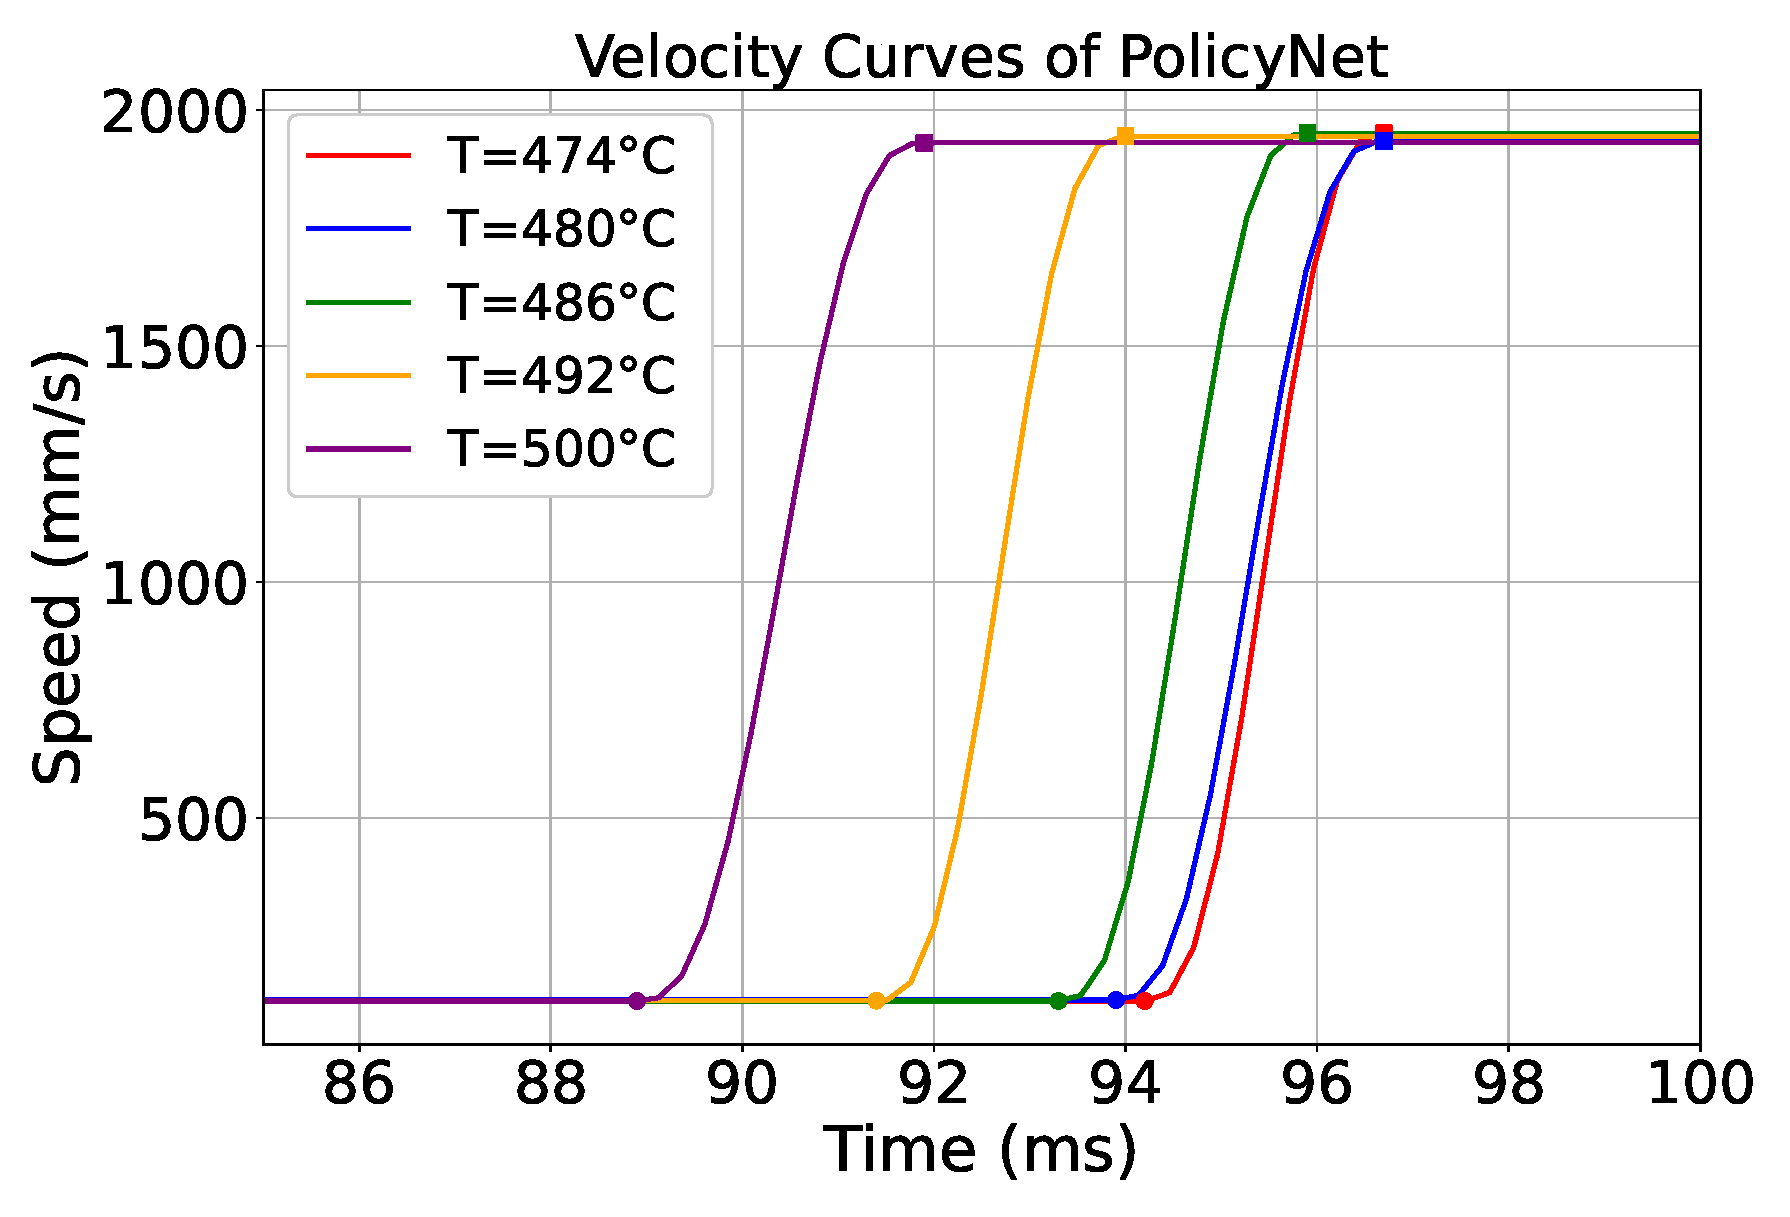
\includegraphics[width=\linewidth]{NetworkSpeed.eps}}
% \caption{Action Curves of the Policy Network Generated at  Different Temperatures (474°C, 480°C, 486°C, 492°C, 500°C).}
% \label{fig:NetworkSpeed}
% \end{figure}

% 与粒子群优化（PSO）算法\cite{wang2018particle}的对比揭示了二者特性的差异。如图\ref{fig:PSOSpeed_b}所示，PSO倾向于生成加速更早的速度曲线，导致锻造时间更短。

A comparison with the particle swarm optimization (PSO) algorithm
\cite{wang2018particle} reveals distinct characteristics between the two
approaches. As shown in Fig. \ref{fig:PSOSpeed_b}, PSO tends to generate
speed profiles with earlier acceleration phases, resulting in shorter
forging times.

% \begin{figure}[htbp]
% \centerline{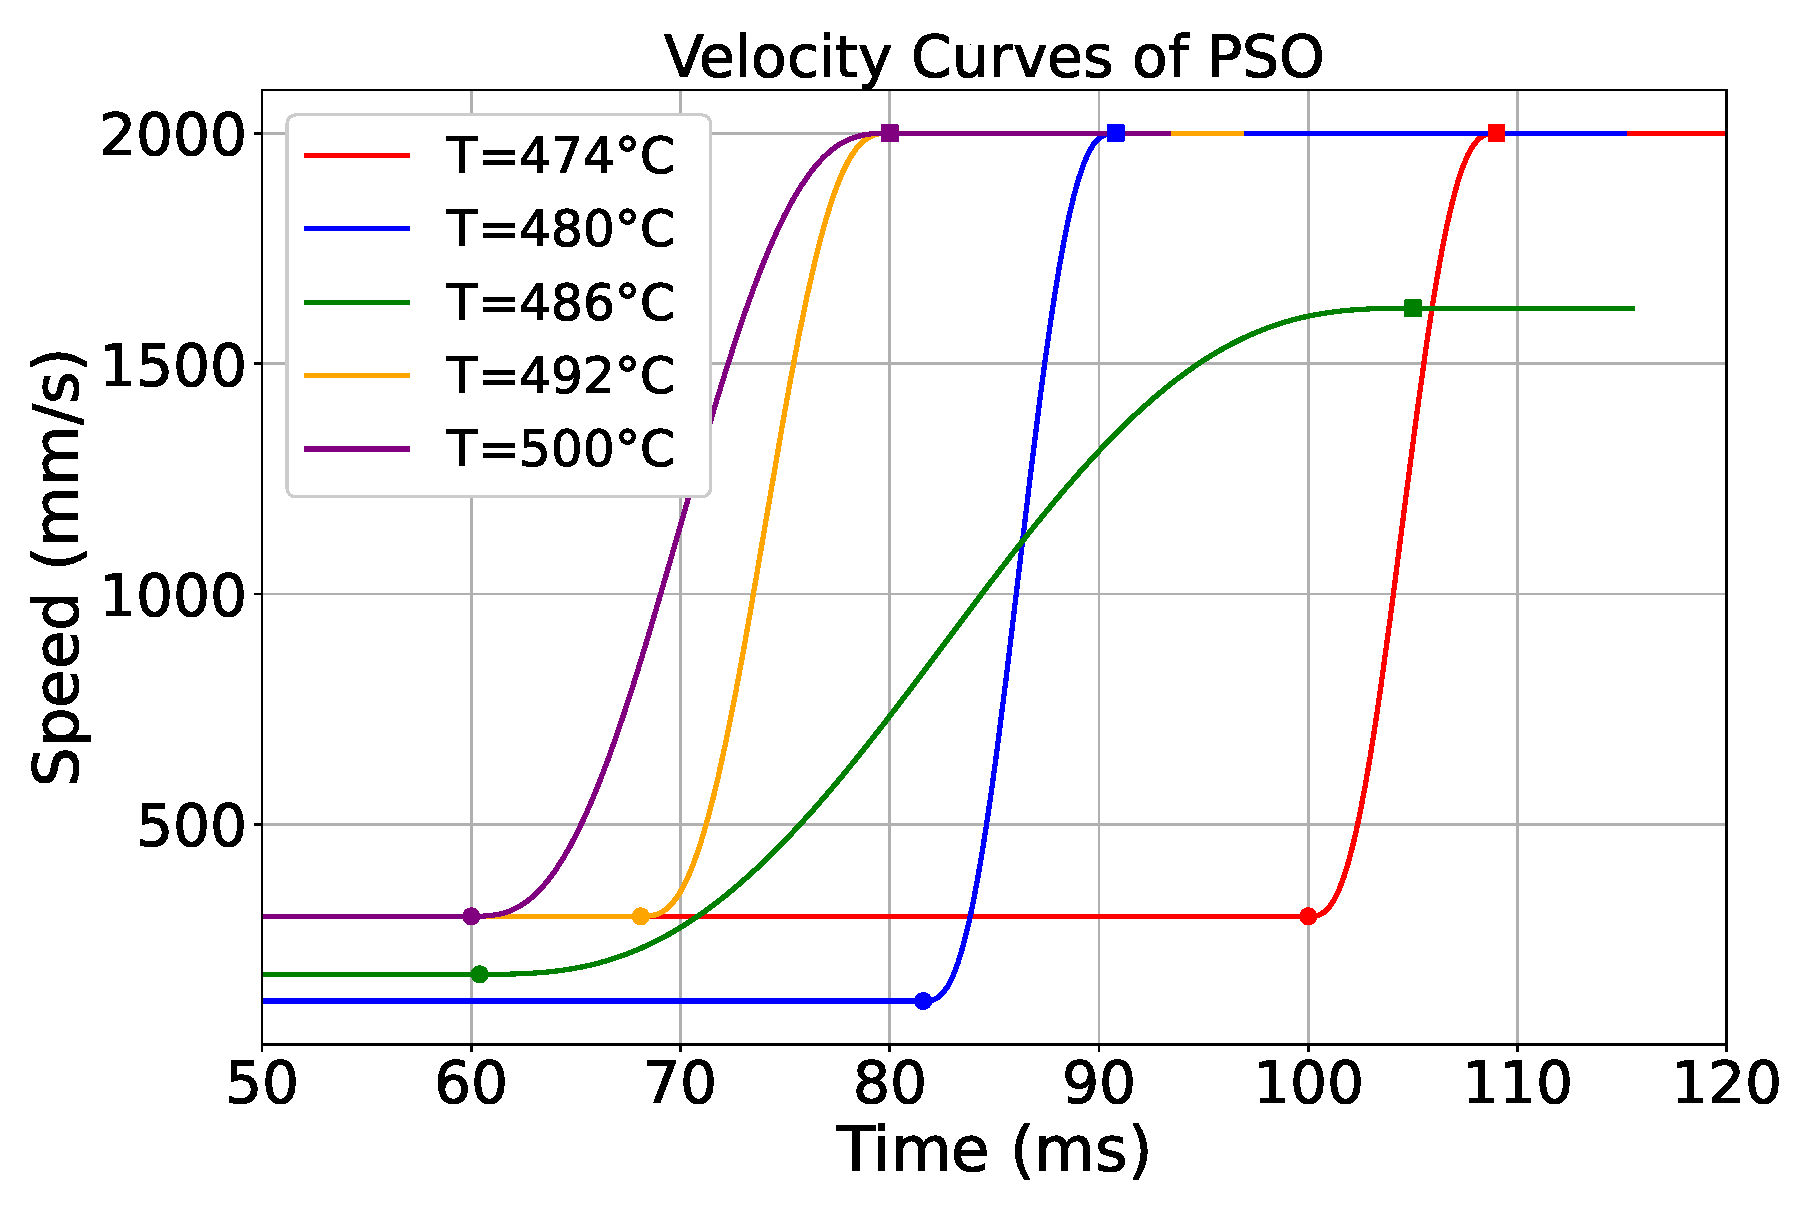
\includegraphics[width=\linewidth]{PSOSpeed.eps}}
% \caption{Action Curves of the PSO Generated at  Different Temperatures (474°C, 480°C, 486°C, 492°C, 500°C).}
% \label{fig:PSOSpeed}
% \end{figure}



% \begin{figure}[htbp]
%     \centering
%     \begin{minipage}{0.48\columnwidth}
%         \centering
%         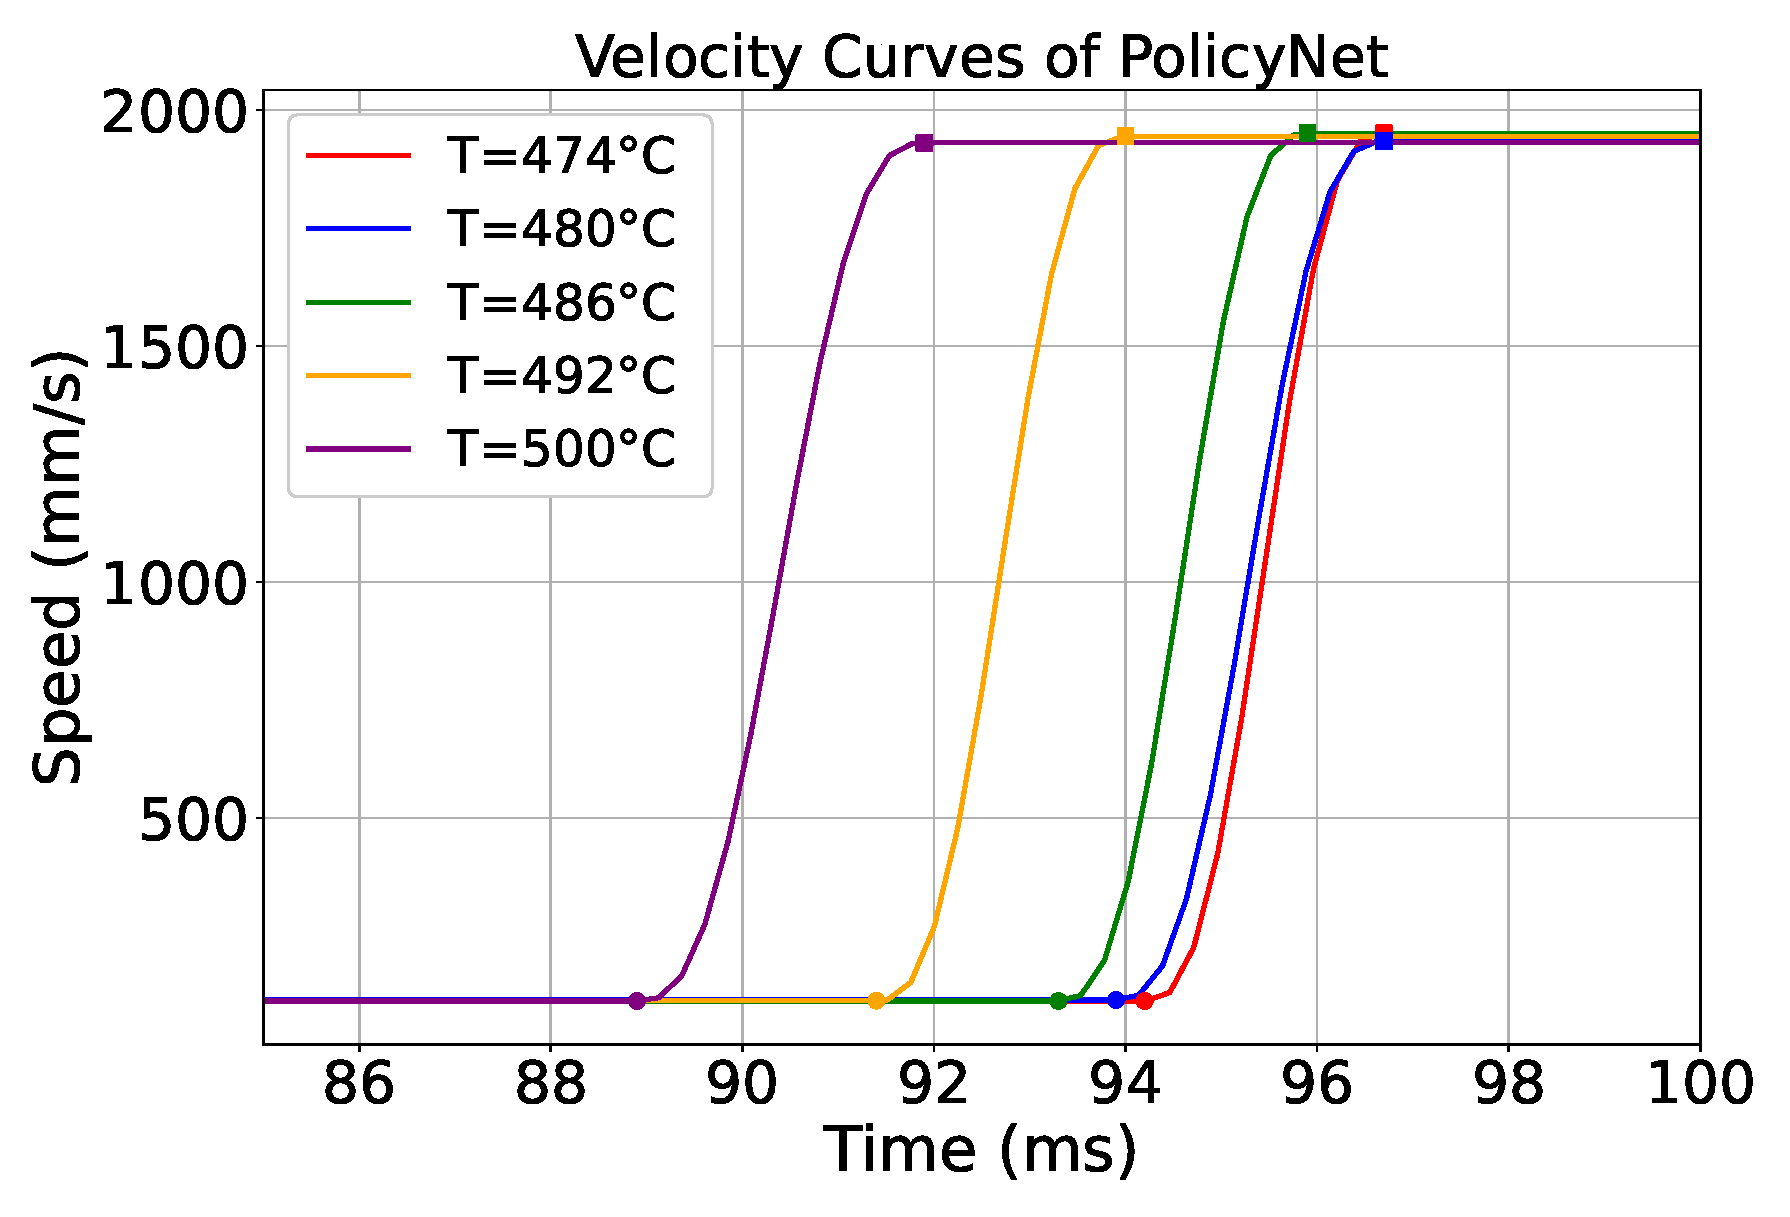
\includegraphics[width=\linewidth]{NetworkSpeed.eps}
%         \caption{Action Curves of the Policy Network Generated at Different Temperatures (474°C, 480°C, 486°C, 492°C, 500°C).}
%         \label{fig:NetworkSpeed}
%     \end{minipage}
%     \hfill
%     \begin{minipage}{0.48\columnwidth}
%         \centering
%         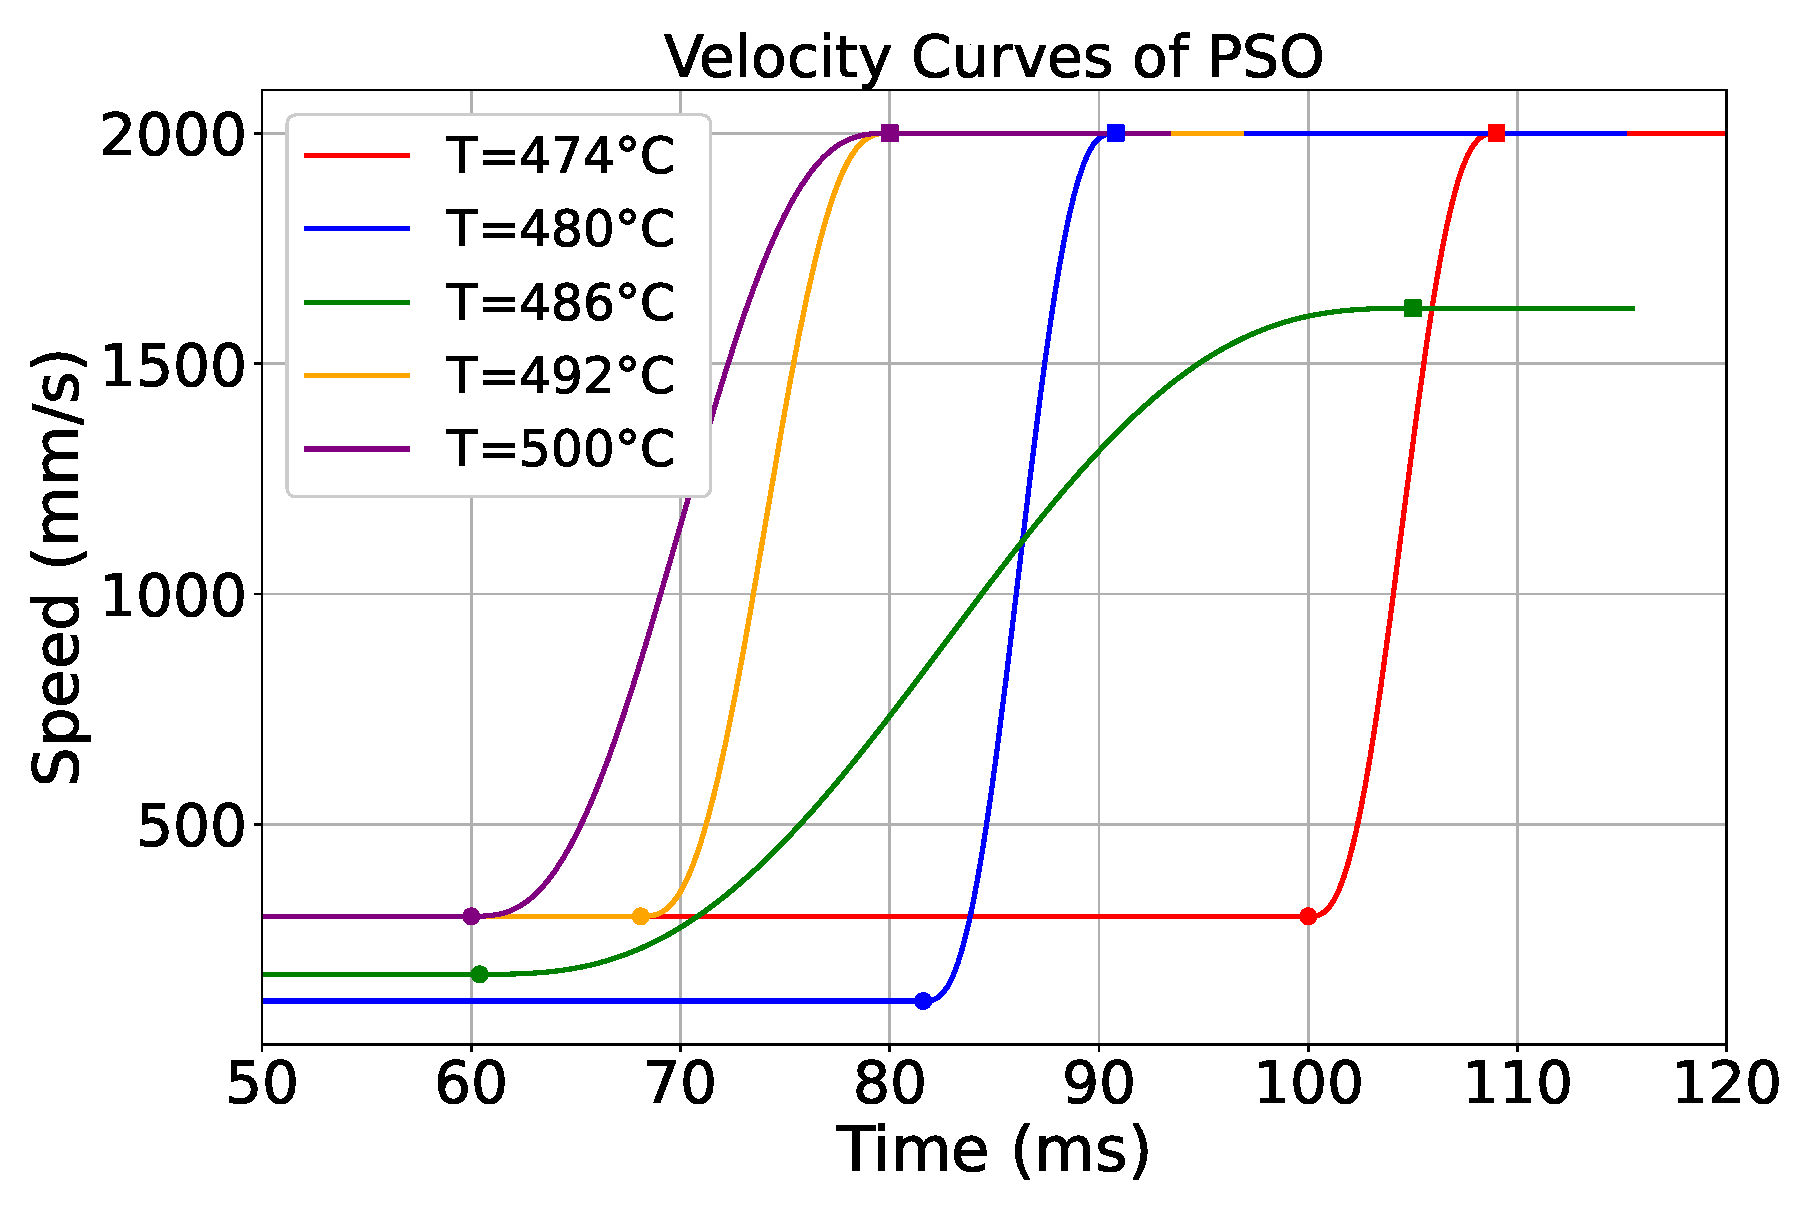
\includegraphics[width=\linewidth]{PSOSpeed.eps}
%         \caption{Action Curves of the PSO Generated at Different Temperatures (474°C, 480°C, 486°C, 492°C, 500°C).}
%         \label{fig:PSOSpeed}
%     \end{minipage}
% \end{figure}


\begin{figure}[htbp]
    \centering
    \begin{subfigure}{0.48\columnwidth}
        \centering
        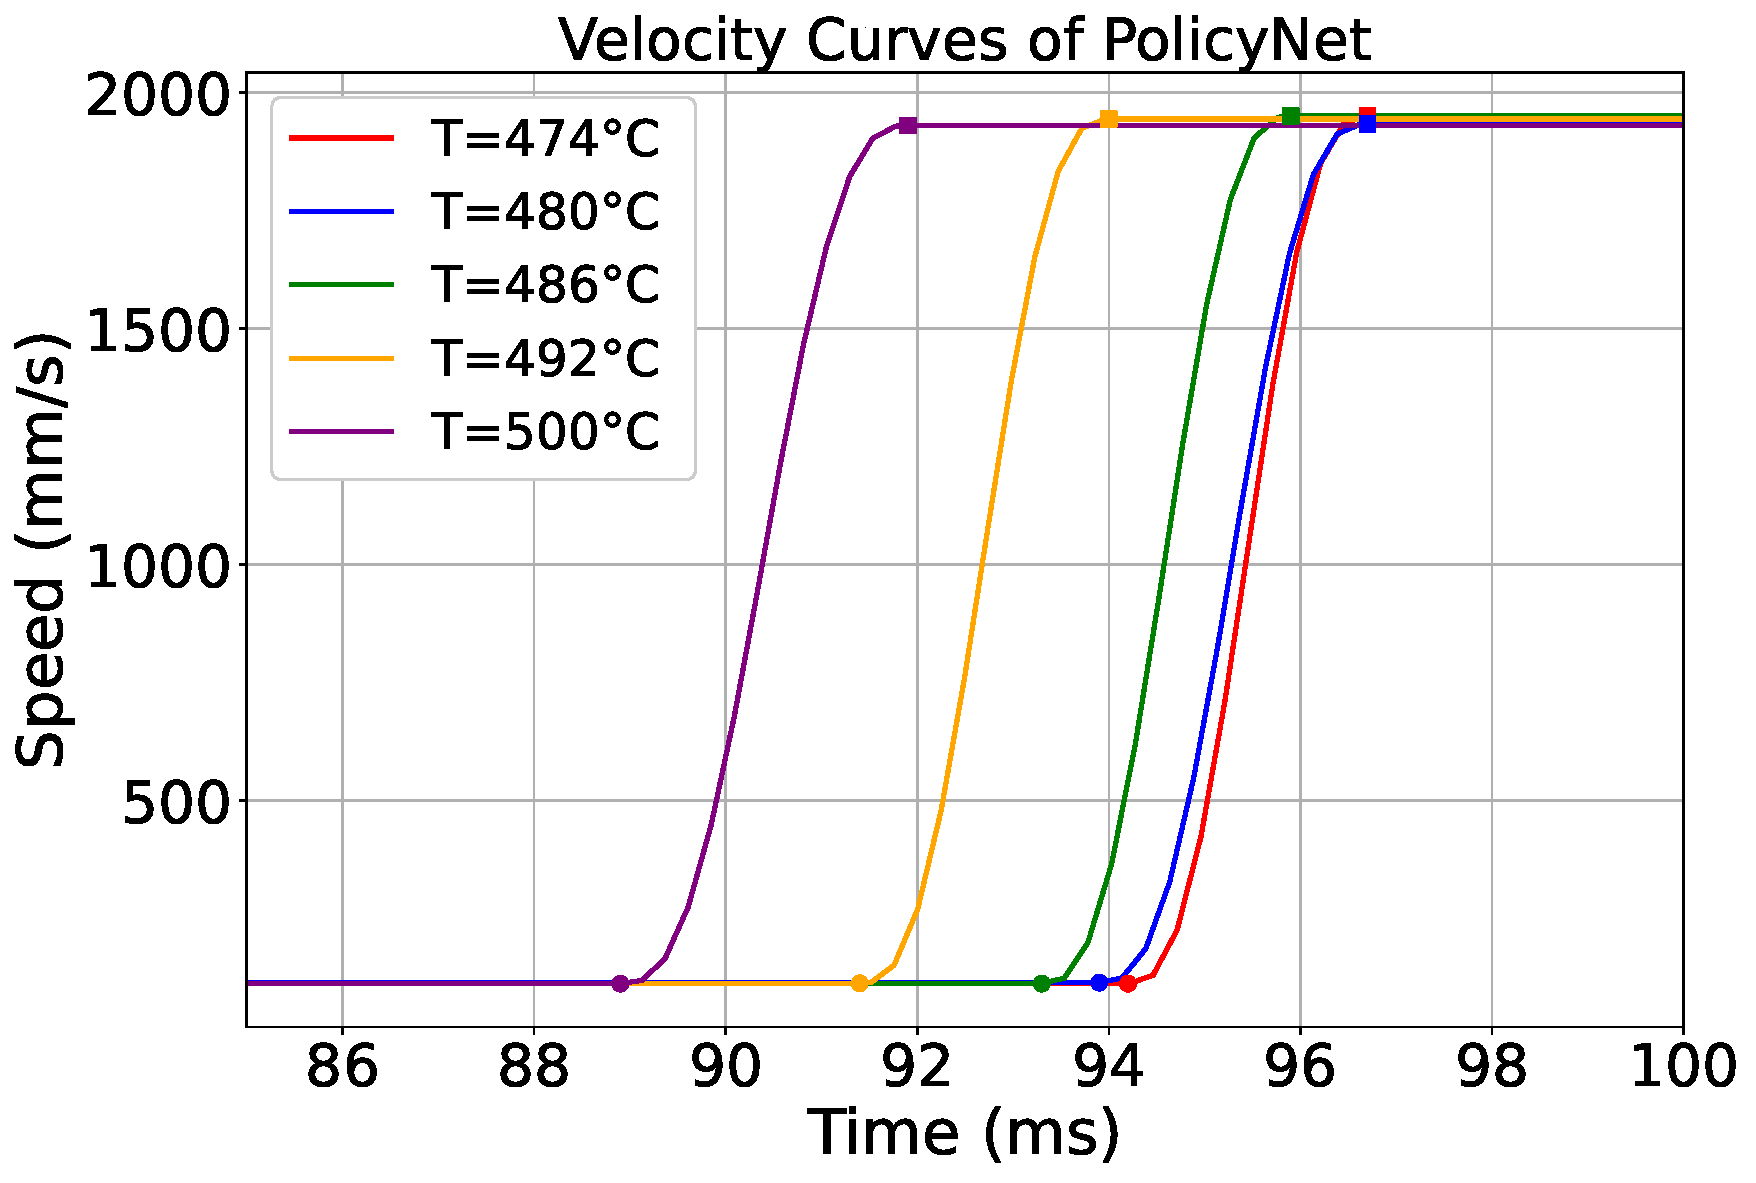
\includegraphics[width=\linewidth]{NetworkSpeed.pdf}
        \caption{Policy Network}
        \label{fig:NetworkSpeed_a}
    \end{subfigure}
    \hfill
    \begin{subfigure}{0.48\columnwidth}
        \centering
        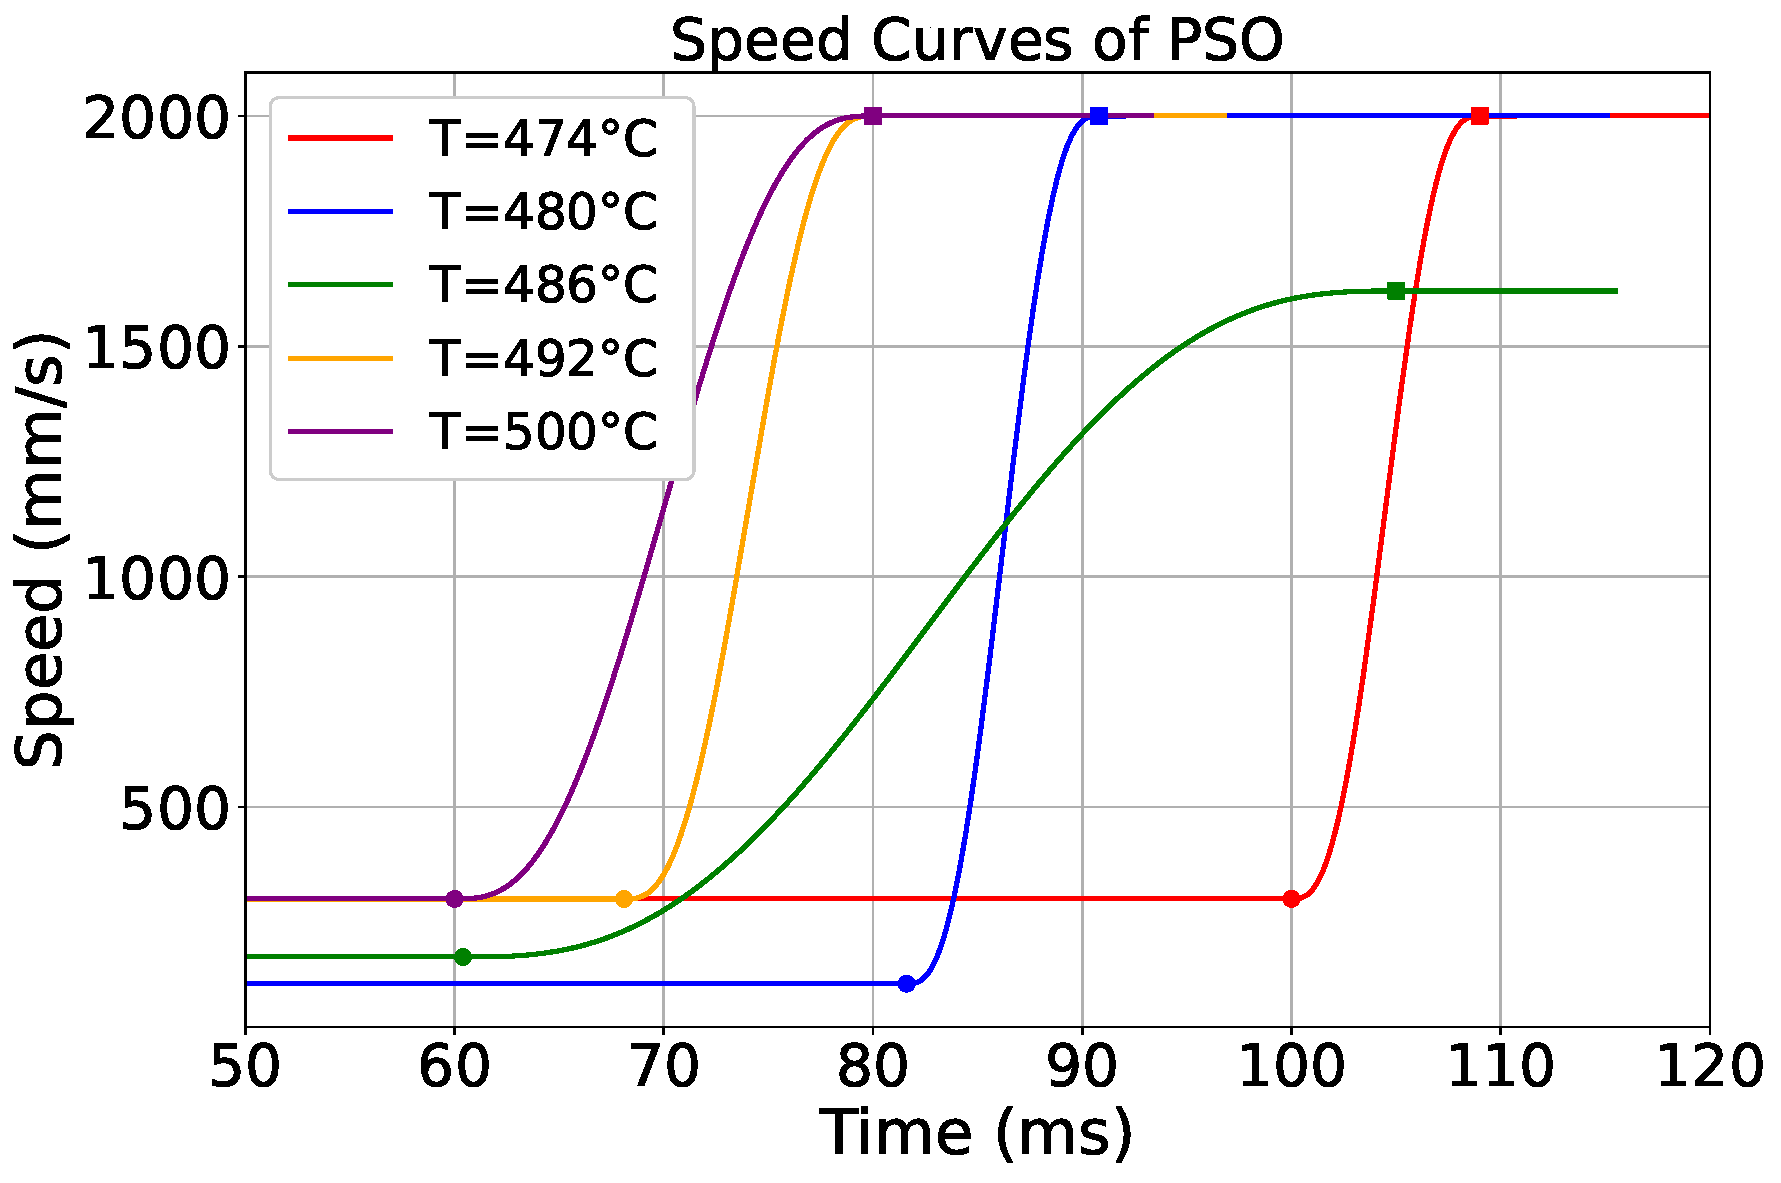
\includegraphics[width=\linewidth]{PSOSpeed.pdf}
        \caption{PSO}
        \label{fig:PSOSpeed_b}
    \end{subfigure}
    \caption{Action curves generated at different temperatures (474°C, 480°C, 486°C, 492°C, 500°C). (a) Policy network; (b) Particle swarm optimization.}
    \label{fig:combined_curves}
\end{figure}

% 工艺性能上（表\ref{tab:Method Comparison}），PSO在锻造时间与损伤率（$0\%$，决策网络为$8\%$）上略优。决策效率上，PSO需约$0.9\text{s}$达到决策网络性能（图\ref{fig:PSO-Objective}），$2.5\text{s}$达最优，而决策网络仅需$0.097\text{s}$，效率相差近一个数量级。

In terms of process performance (Table \ref{tab:Method Comparison}), PSO
slightly outperforms in forging time and achieves a lower damage rate
($0\%$ vs. $8\%$ for the policy network). Regarding decision efficiency,
PSO requires approximately $0.9\text{s}$ to reach the performance level
of the policy network (Fig. \ref{fig:PSO-Objective}) and $2.5\text{s}$ to
achieve its optimum, whereas the policy network requires only
$0.097\text{s}$—nearly an order of magnitude faster.

\begin{table}[htbp]
\centering
\caption{Method Comparison}
\setlength{\tabcolsep}{3.5pt} % 缩小列间距（默认约6pt，可根据需要调整）
\begin{tabular}{c c c c}
\toprule
\textbf{Method} & \textbf{Forge Time} & \textbf{Decision Time} & \textbf{Damage Rate}\\
& (mean$\pm$std,ms) & (mean$\pm$std,ms) & (\%)\\
\midrule
PolicyNet & 121.91 $\pm$ 6.63 & 97.37 $\pm$ 3.86 & 8.00 \\
PSO       & 108.72 $\pm$ 11.55 & 2580 $\pm$ 1370  & 0.00 \\
\bottomrule
\end{tabular}
\label{tab:Method Comparison}
\end{table}


\begin{figure}[htbp]
\centerline{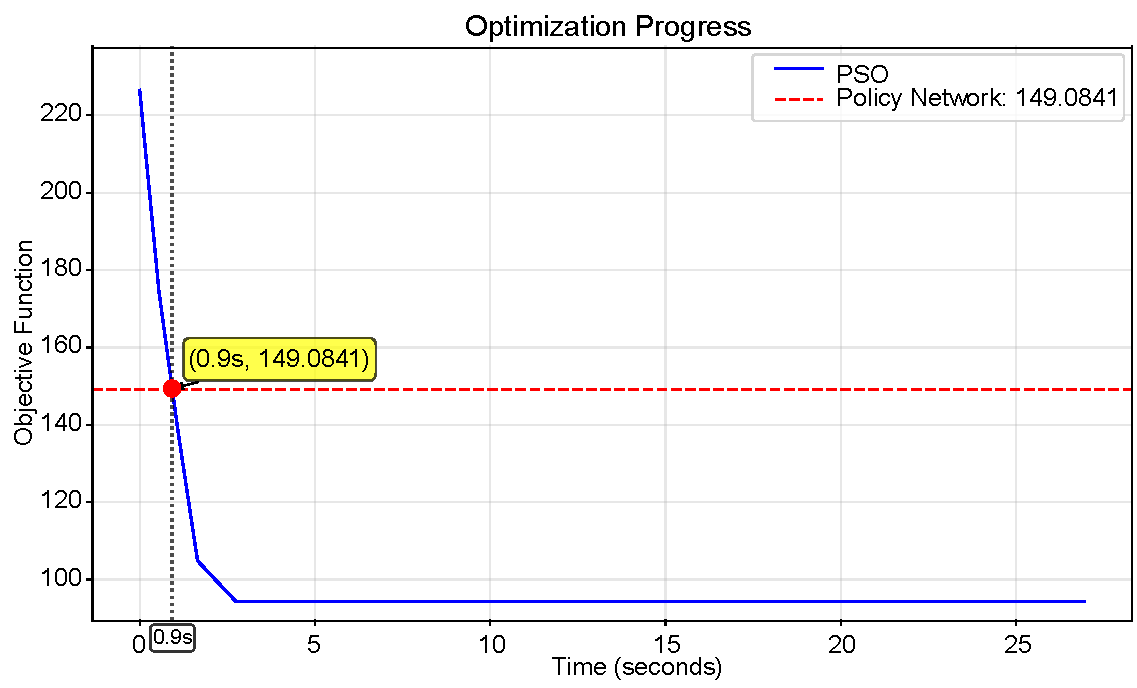
\includegraphics[width=\linewidth]{PSO-Objective-2.pdf}}
\caption{Objective function comparison.}
\label{fig:PSO-Objective}
\end{figure}
In summary, while PSO achieves superior process quality, its extended
decision time hinders real-time application. In contrast, the policy
network provides rapid decision-making while maintaining acceptable
process quality, demonstrating greater suitability for practical
scenarios.

  \section*{Conclusion}
% 本研究构建了一套基于安全离线强化学习的锻造优化控制框架，通过深度算子网络构建高效代理模型，结合参数化动作空间与拉格朗日约束优化方法，实现了在严格满足损伤约束条件下的下压速度曲线实时决策。实验结果表明，该方案在保证可接受工艺质量的同时，具备显著的决策效率优势，为锻造场景下的智能优化控制提供了可行的技术路径。

This study presents a safe offline reinforcement learning framework for
forging optimization. By integrating a deep operator network-based
surrogate model with a parameterized action space and Lagrangian
constraint optimization, the framework enables real-time generation of
forging speed curves under strict damage constraints. Experimental
results demonstrate that the method maintains acceptable process quality
while achieving significant gains in decision-making efficiency, offering
a viable technical pathway for intelligent optimization in forging
applications.

  \Acknowledgements{This work was supported by the National Science and Technology Major Project of the Ministry of Science and Technology of China (2024ZD0608100), the National Natural Science Foundation of China (62506031, 62332017, U22A2022), Fellowship from the China Postdoctoral Science Foundation (2026T190405), the Postdoctoral Fellowship Program of CPSF under Grant Number GZC20251093.}

\fi

\bibliographystyle{scis}
\bibliography{ref}

\end{document}
